\documentclass[11pt,aspectratio=169]{beamer}
% WiL architecture deck, 18 November 2026.
% Purpose: open the black box. Every component of the stack is explained once,
% with the data that enters and leaves it; section 2 then attaches each result
% with a mechanism to the component that explains it (s7_results.tex).
% Component IDs (ORB-3, RTAB-6, ...) are stable: reference them, never page
% numbers.
% =============================================================================
% Shared preamble for update_181126: the architecture deck.
% Visual vocabulary follows the two references in this folder:
%   image copy.png  -> 1.1 (function columns, colour-coded data lines)
%   image.png       -> sub-component slides (one stage panel: picture + caption)
% =============================================================================
\usetheme{default}
\usecolortheme{seagull}
\setbeamertemplate{navigation symbols}{}
\setbeamertemplate{footline}[frame number]
\setbeamerfont{frametitle}{size=\large,series=\bfseries}
\setbeamercolor{frametitle}{fg=black!85}
\usepackage[T1]{fontenc}
\usepackage[utf8]{inputenc}
\usepackage{booktabs}
\usepackage{array}
\usepackage{multirow}
\usepackage{siunitx}
\usepackage{graphicx}
\usepackage{xcolor}
\usepackage{amssymb}
\usepackage{adjustbox}
\usepackage[most]{tcolorbox}
\usepackage{tikz}
\usetikzlibrary{arrows.meta,positioning,fit,calc,backgrounds,
                decorations.pathreplacing,shapes.geometric,shadows}
\sisetup{detect-all,range-phrase=--,range-units=single,retain-explicit-plus}
\DeclareSIUnit{\mebi}{Mi}
\newcommand{\repo}[1]{\texttt{\detokenize{#1}}}
\newcommand{\src}[1]{\vfill{\tiny\color{black!50}#1}}

% ---------------------------------------------------------------- colours
% function columns (1.1), after image copy.png
\definecolor{sensorcol}{HTML}{2FB5E8}
\definecolor{perccol}{HTML}{26A69A}
\definecolor{plancol}{HTML}{F2735A}
\definecolor{ctrlcol}{HTML}{8FA3BA}
\definecolor{mapcol}{HTML}{34495E}
% one colour per system
\definecolor{orbc}{HTML}{D6336C}
\definecolor{vinsc}{HTML}{E67E22}
\definecolor{rtabc}{HTML}{27AE60}
\definecolor{navc}{HTML}{2E86DE}
\definecolor{sysc}{HTML}{5D6D7E}
% data-line colours: one per kind of data
\definecolor{dimg}{HTML}{E74C3C}
\definecolor{dimu}{HTML}{F39C12}
\definecolor{dwhl}{HTML}{16A085}
\definecolor{dpose}{HTML}{8E44AD}
\definecolor{dmap}{HTML}{2C3E50}
\definecolor{dcmd}{HTML}{2E86DE}
% marks
\definecolor{ourc}{HTML}{E0A100}
\definecolor{hlc}{HTML}{C0392B}
\definecolor{offc}{HTML}{AAB7B8}
\definecolor{good}{HTML}{1E8449}
\definecolor{bad}{HTML}{C0392B}

% ---------------------------------------------------------------- tikz styles
\tikzset{
  box/.style={draw=black!45, rounded corners=2pt, align=center, font=\scriptsize,
              inner sep=2pt, minimum height=8mm, text width=22mm, fill=white},
  arr/.style={-{Latex[length=1.8mm]}, thick, black!65},
  darr/.style={arr, dashed},
  rate/.style={font=\tiny, fill=white, inner sep=1pt, text=black!75, align=center},
  % "added by this project" and "switched off"
  ours/.style={draw=ourc, dashed, line width=1.2pt},
  off/.style={draw=offc, dashed, fill=offc!15, text=black!45},
  % the current component
  hl/.style={draw=hlc, line width=1.6pt, fill=yellow!35},
  % locator chips
  chip/.style={draw=black!35, rounded corners=1.5pt, align=center, font=\scriptsize,
               inner sep=1.5pt, minimum height=8mm, text width=17mm},
  grouplbl/.style={font=\scriptsize\bfseries, text=black!60},
  brace/.style={decorate, decoration={brace, amplitude=3pt, raise=2pt}, thick, black!40},
  % small drawing helpers for the stage panels
  pt/.style={circle, fill=#1, inner sep=0pt, minimum size=1.6mm},
  pt/.default=black,
  cam/.style={isosceles triangle, shape border rotate=#1, draw=black!70, fill=white,
              minimum width=4mm, minimum height=4mm, inner sep=0pt},
  cam/.default=0,
}
% Every component has a style of its own name, empty by default.
% \hl{ORB3} inside a frame turns that one component yellow-and-red, so the
% locator strip and the block diagram both show "you are here".
\tikzset{ORB1/.style={},ORB2/.style={},ORB3/.style={},ORB4/.style={},
         ORB5/.style={},ORB6/.style={},ORB7/.style={},ORB8/.style={},
         VINS1/.style={},VINS2/.style={},VINS3/.style={},VINS4/.style={},
         VINS5/.style={},VINS6/.style={},VINS7/.style={},
         RTAB1/.style={},RTAB2/.style={},RTAB3/.style={},RTAB4/.style={},
         RTAB5/.style={},RTAB6/.style={},RTAB7/.style={},RTAB8/.style={},RTAB9/.style={},
         NAV1/.style={},NAV2/.style={},NAV3/.style={},NAV4/.style={},
         NAV5/.style={},NAV6/.style={},NAV7/.style={},NAV8/.style={}}
\newcommand{\hl}[1]{\tikzset{#1/.style={hl}}}

% ---------------------------------------------------------------- panels
% The stage panel: a coloured header, one picture, one caption.  The picture is
% scaled to fit, never to overflow.
\newtcolorbox{stagepanel}[2][]{enhanced, colback=white, colframe=#2,
  boxrule=0.8pt, arc=2pt, left=3pt, right=3pt, top=2pt, bottom=2pt,
  fonttitle=\scriptsize\bfseries, coltitle=white, title={#1}}
\newcommand{\stage}[4]{% #1 colour, #2 header, #3 tikz body, #4 caption
  \begin{stagepanel}[#2]{#1}
    \centering
    \adjustbox{max width=\linewidth, max height=3.3cm}{#3}\par\vspace{2pt}
    {\scriptsize #4}
  \end{stagepanel}}
% The right-hand column of a component slide.
\newtcolorbox{linkpanel}{enhanced, colback=mapcol!5, colframe=mapcol,
  boxrule=0.8pt, arc=2pt, left=3pt, right=3pt, top=2pt, bottom=2pt,
  fonttitle=\scriptsize\bfseries, coltitle=white, title={LINK TO RESULTS}}
\newcommand{\side}[5]{% #1 why, #2 in, #3 out, #4 can go wrong, #5 signal
  {\scriptsize\textbf{\color{mapcol}WHY IT EXISTS}\par\footnotesize #1\par}
  \vspace{0.3em}
  {\scriptsize\raggedright\textbf{\color{mapcol}IN}\quad #2\par
   \textbf{\color{mapcol}OUT}\enspace #3\par}
  \vspace{0.3em}
  \begin{linkpanel}\scriptsize\raggedright
    \textbf{Can go wrong:} #4\par\smallskip
    \textbf{Signal:} #5\par\smallskip
    \textbf{Results:} \resref
  \end{linkpanel}}
% A whole component slide body: strip, then panel (left) + side (right).
\newcommand{\compbody}[9]{% #1 strip macro, #2 colour, #3 tikz, #4 caption,
                          % #5 why, #6 in, #7 out, #8 wrong, #9 signal
  #1\par\vspace{0.25em}
  \begin{columns}[T]
    \column{0.55\textwidth}\stage{#2}{HOW IT WORKS}{#3}{#4}
    \column{0.43\textwidth}\side{#5}{#6}{#7}{#8}{#9}
  \end{columns}}

% One lane of the "three clocks" timeline (1.1): y, label, rate in Hz, colour.
\newcommand{\lane}[4]{%
  \node[anchor=east, align=right] at (-0.02,#1) {#2};
  \draw[black!15] (0,#1) -- (1,#1);
  \foreach \k in {1,...,#3} \draw[#4, line width=0.7pt]
    ({(\k-0.5)/#3},#1-0.18) -- ({(\k-0.5)/#3},#1+0.18);}

% ---------------------------------------------------------------- results
% A component slide's "Results" line.  \res{...} inside a frame sets it for that
% frame only; \R{n}{text} links to the finding slide labelled Rn.
\newcommand{\resref}{{\color{black!40}\emph{no finding yet}}}
\newcommand{\res}[1]{\renewcommand{\resref}{#1}}
\newcommand{\R}[2]{\hyperlink{R#1}{\textbf{\color{hlc}R#1}}~#2}
\graphicspath{{../../final_report/figures/}{../experiment_4/fig/}}
% A finding slide body, under its strip(s): picture left, two panels right.
\newcommand{\finding}[5]{% #1 colour, #2 picture, #3 what we saw, #4 why, #5 caveat
  \begin{columns}[T]
    \column{0.57\textwidth}\centering
      \adjustbox{max width=\linewidth, max height=0.50\textheight}{#2}
    \column{0.42\textwidth}
      \begin{stagepanel}[WHAT WE SAW]{mapcol}\scriptsize\raggedright #3\end{stagepanel}
      \vspace{-0.4em}
      \begin{stagepanel}[WHY: INSIDE THE BLOCK]{#1}\scriptsize\raggedright #4\end{stagepanel}
  \end{columns}
  \vspace{0.2em}
  {\scriptsize\color{black!70}\textbf{\color{bad}Careful:} #5\par}}

% =============================================================================
% Locator strips: one row of chips per system, in data-flow order, grouped by
% thread.  On a component slide, \hl{ID} before the strip marks "you are here".
% =============================================================================
\newcommand{\orbstrip}{%
\adjustbox{max width=\textwidth}{%
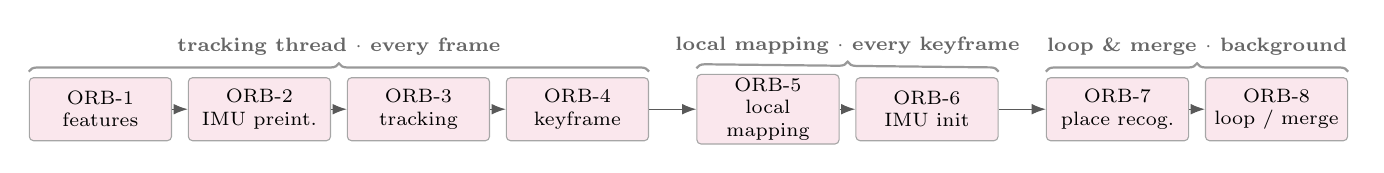
\begin{tikzpicture}[node distance=2mm]
  \node[chip, fill=orbc!12, ORB1] (c1) {ORB-1\\features};
  \node[chip, fill=orbc!12, ORB2, right=of c1] (c2) {ORB-2\\IMU preint.};
  \node[chip, fill=orbc!12, ORB3, right=of c2] (c3) {ORB-3\\tracking};
  \node[chip, fill=orbc!12, ORB4, right=of c3] (c4) {ORB-4\\keyframe};
  \node[chip, fill=orbc!12, ORB5, right=6mm of c4] (c5) {ORB-5\\local mapping};
  \node[chip, fill=orbc!12, ORB6, right=of c5] (c6) {ORB-6\\IMU init};
  \node[chip, fill=orbc!12, ORB7, right=6mm of c6] (c7) {ORB-7\\place recog.};
  \node[chip, fill=orbc!12, ORB8, right=of c7] (c8) {ORB-8\\loop / merge};
  \draw[brace] (c1.north west) -- node[above=4pt, grouplbl]{tracking thread $\cdot$ every frame} (c4.north east);
  \draw[brace] (c5.north west) -- node[above=4pt, grouplbl]{local mapping $\cdot$ every keyframe} (c6.north east);
  \draw[brace] (c7.north west) -- node[above=4pt, grouplbl]{loop \& merge $\cdot$ background} (c8.north east);
  \foreach \a/\b in {c1/c2,c2/c3,c3/c4,c4/c5,c5/c6,c6/c7,c7/c8} \draw[arr, thin] (\a) -- (\b);
\end{tikzpicture}}}

\newcommand{\vinsstrip}{%
\adjustbox{max width=\textwidth}{%
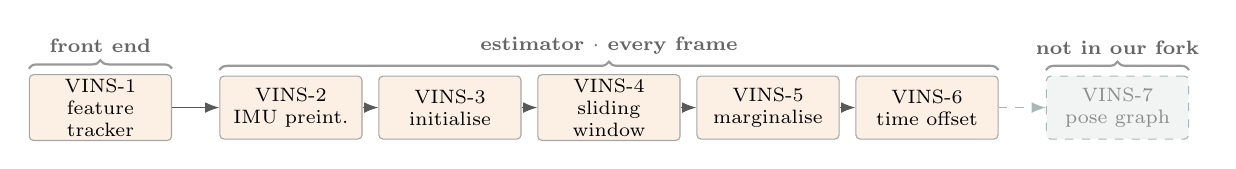
\begin{tikzpicture}[node distance=2mm]
  \node[chip, fill=vinsc!12, VINS1] (c1) {VINS-1\\feature tracker};
  \node[chip, fill=vinsc!12, VINS2, right=6mm of c1] (c2) {VINS-2\\IMU preint.};
  \node[chip, fill=vinsc!12, VINS3, right=of c2] (c3) {VINS-3\\initialise};
  \node[chip, fill=vinsc!12, VINS4, right=of c3] (c4) {VINS-4\\sliding window};
  \node[chip, fill=vinsc!12, VINS5, right=of c4] (c5) {VINS-5\\marginalise};
  \node[chip, fill=vinsc!12, VINS6, right=of c5] (c6) {VINS-6\\time offset};
  \node[chip, off, VINS7, right=6mm of c6] (c7) {VINS-7\\pose graph};
  \draw[brace] (c1.north west) -- node[above=4pt, grouplbl]{front end} (c1.north east);
  \draw[brace] (c2.north west) -- node[above=4pt, grouplbl]{estimator $\cdot$ every frame} (c6.north east);
  \draw[brace] (c7.north west) -- node[above=4pt, grouplbl]{not in our fork} (c7.north east);
  \foreach \a/\b in {c1/c2,c2/c3,c3/c4,c4/c5,c5/c6} \draw[arr, thin] (\a) -- (\b);
  \draw[darr, thin, offc] (c6) -- (c7);
\end{tikzpicture}}}

\newcommand{\rtabstrip}{%
\adjustbox{max width=\textwidth}{%
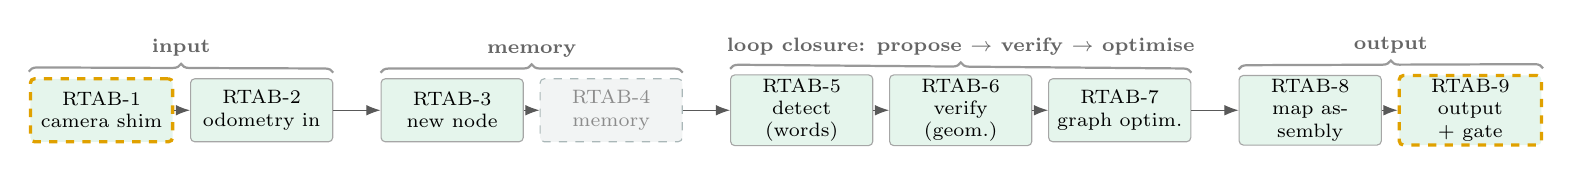
\begin{tikzpicture}[node distance=2mm]
  \node[chip, fill=rtabc!12, ours, RTAB1] (c1) {RTAB-1\\camera shim};
  \node[chip, fill=rtabc!12, RTAB2, right=of c1] (c2) {RTAB-2\\odometry in};
  \node[chip, fill=rtabc!12, RTAB3, right=6mm of c2] (c3) {RTAB-3\\new node};
  \node[chip, off, RTAB4, right=of c3] (c4) {RTAB-4\\memory};
  \node[chip, fill=rtabc!12, RTAB5, right=6mm of c4] (c5) {RTAB-5\\detect (words)};
  \node[chip, fill=rtabc!12, RTAB6, right=of c5] (c6) {RTAB-6\\verify (geom.)};
  \node[chip, fill=rtabc!12, RTAB7, right=of c6] (c7) {RTAB-7\\graph optim.};
  \node[chip, fill=rtabc!12, RTAB8, right=6mm of c7] (c8) {RTAB-8\\map assembly};
  \node[chip, fill=rtabc!12, ours, RTAB9, right=of c8] (c9) {RTAB-9\\output + gate};
  \draw[brace] (c1.north west) -- node[above=4pt, grouplbl]{input} (c2.north east);
  \draw[brace] (c3.north west) -- node[above=4pt, grouplbl]{memory} (c4.north east);
  \draw[brace] (c5.north west) -- node[above=4pt, grouplbl]{loop closure: propose $\rightarrow$ verify $\rightarrow$ optimise} (c7.north east);
  \draw[brace] (c8.north west) -- node[above=4pt, grouplbl]{output} (c9.north east);
  \foreach \a/\b in {c1/c2,c2/c3,c3/c4,c4/c5,c5/c6,c6/c7,c7/c8,c8/c9} \draw[arr, thin] (\a) -- (\b);
\end{tikzpicture}}}

\newcommand{\navstrip}{%
\adjustbox{max width=\textwidth}{%
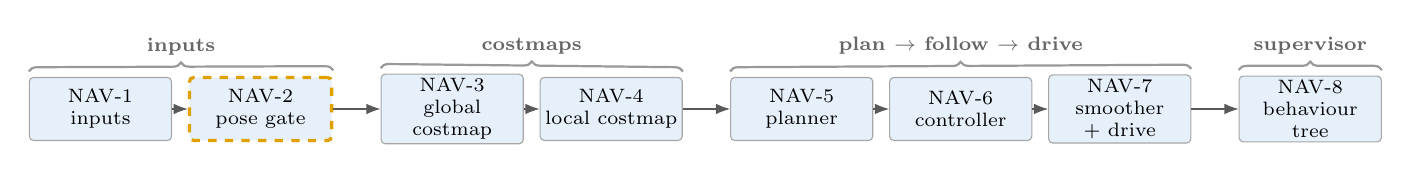
\begin{tikzpicture}[node distance=2mm]
  \node[chip, fill=navc!12, NAV1] (c1) {NAV-1\\inputs};
  \node[chip, fill=navc!12, ours, NAV2, right=of c1] (c2) {NAV-2\\pose gate};
  \node[chip, fill=navc!12, NAV3, right=6mm of c2] (c3) {NAV-3\\global costmap};
  \node[chip, fill=navc!12, NAV4, right=of c3] (c4) {NAV-4\\local costmap};
  \node[chip, fill=navc!12, NAV5, right=6mm of c4] (c5) {NAV-5\\planner};
  \node[chip, fill=navc!12, NAV6, right=of c5] (c6) {NAV-6\\controller};
  \node[chip, fill=navc!12, NAV7, right=of c6] (c7) {NAV-7\\smoother + drive};
  \node[chip, fill=navc!12, NAV8, right=6mm of c7] (c8) {NAV-8\\behaviour tree};
  \draw[brace] (c1.north west) -- node[above=4pt, grouplbl]{inputs} (c2.north east);
  \draw[brace] (c3.north west) -- node[above=4pt, grouplbl]{costmaps} (c4.north east);
  \draw[brace] (c5.north west) -- node[above=4pt, grouplbl]{plan $\rightarrow$ follow $\rightarrow$ drive} (c7.north east);
  \draw[brace] (c8.north west) -- node[above=4pt, grouplbl]{supervisor} (c8.north east);
  \foreach \a/\b in {c1/c2,c2/c3,c3/c4,c4/c5,c5/c6,c6/c7,c7/c8} \draw[arr, thin] (\a) -- (\b);
\end{tikzpicture}}}


\title{How the WiL system works}
\subtitle{The architecture, component by component \textperiodcentered\
  ORB-SLAM3, VINS-Fusion, RTAB-Map and Nav2}
\author{Bolton Athit Davies}
\date{18 November 2026 \textperiodcentered\ architecture, then the results it explains}

\begin{document}

\begin{frame}
  \titlepage
\end{frame}

% ---------------------------------------------------------------- how to read
\begin{frame}{How to read this deck}
  \begin{columns}[T]
    \column{0.50\textwidth}
      \small
      \textbf{The order}
      \begin{enumerate}
        \item[1.1] the whole system on one page, with its data rates
        \item[1.2] ORB-SLAM3 \hfill front end, option A
        \item[1.3] VINS-Fusion \hfill front end, option B
        \item[1.4] RTAB-Map \hfill the map you come back to
        \item[1.5] Nav2 \hfill planning and driving
      \end{enumerate}
      \vspace{0.4em}
      Each section: one block diagram, then one slide per block, then the
      configuration we actually run.
      \par\vspace{0.4em}
      \textbf{No results in this deck.} Every block slide has an empty
      \emph{Results} slot; the analysis attaches there later, by component ID.
    \column{0.48\textwidth}
      \small
      \textbf{Every block slide looks like this}
      \par\vspace{0.3em}
      \centering
      \adjustbox{max width=\linewidth}{%
      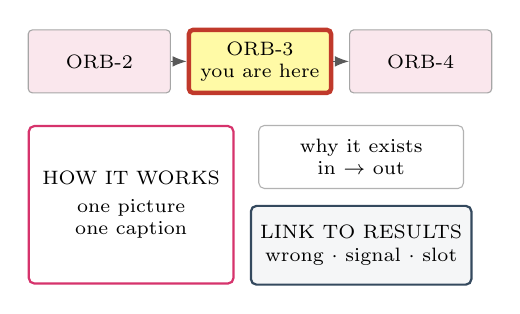
\begin{tikzpicture}[node distance=2mm]
        \node[chip, fill=orbc!12] (a) {ORB-2};
        \node[chip, fill=orbc!12, hl, right=of a] (b) {ORB-3\\you are here};
        \node[chip, fill=orbc!12, right=of b] (c) {ORB-4};
        \draw[arr, thin] (a) -- (b); \draw[arr, thin] (b) -- (c);
        \node[draw=orbc, thick, rounded corners=2pt, minimum width=26mm,
              minimum height=20mm, below=4mm of a.south west, anchor=north west,
              align=center, font=\scriptsize] (p) {HOW IT WORKS\\[2pt]
              one picture\\one caption};
        \node[draw=black!30, rounded corners=2pt, minimum width=26mm,
              minimum height=8mm, right=3mm of p.north east, anchor=north west,
              font=\scriptsize, align=center] (w) {why it exists\\in $\rightarrow$ out};
        \node[draw=mapcol, thick, fill=mapcol!5, rounded corners=2pt,
              minimum width=26mm, minimum height=10mm, below=2mm of w,
              font=\scriptsize, align=center] (l) {LINK TO RESULTS\\wrong $\cdot$ signal $\cdot$ slot};
      \end{tikzpicture}}
      \par\vspace{0.5em}
      \raggedright\scriptsize
      \begin{tabular}{@{}l@{\ \ }l@{}}
        \tikz\node[chip, fill=white, hl, minimum height=4mm, text width=6mm]{};
          & the block this slide explains \\[3pt]
        \tikz\node[chip, fill=white, ours, minimum height=4mm, text width=6mm]{};
          & added by this project, not in the library \\[3pt]
        \tikz\node[chip, off, minimum height=4mm, text width=6mm]{};
          & exists, but switched off in our runs \\
      \end{tabular}
  \end{columns}
\end{frame}

% =============================================================================
% 1.1  THE WHOLE SYSTEM
% Layout after "image copy.png": function columns left to right, sensors first,
% a MAP box underneath, one colour per kind of data.  Rates are from the robot
% SDF (cameras 30, IMU 200, wheel odometry 50 Hz), the VINS/ORB configs, the
% camera shim (4 Hz), rtabmap.launch.py (DetectionRate 1 Hz),
% correction_gate.py (20 Hz), pose_gate.py (2 Hz) and nav2_sim.yaml.
% =============================================================================
\section{1.1 The system}

\begin{frame}{1.1 \;The whole system: from camera pixels to wheel commands}
  \centering
  \adjustbox{max width=\textwidth, max height=0.80\textheight}{%
  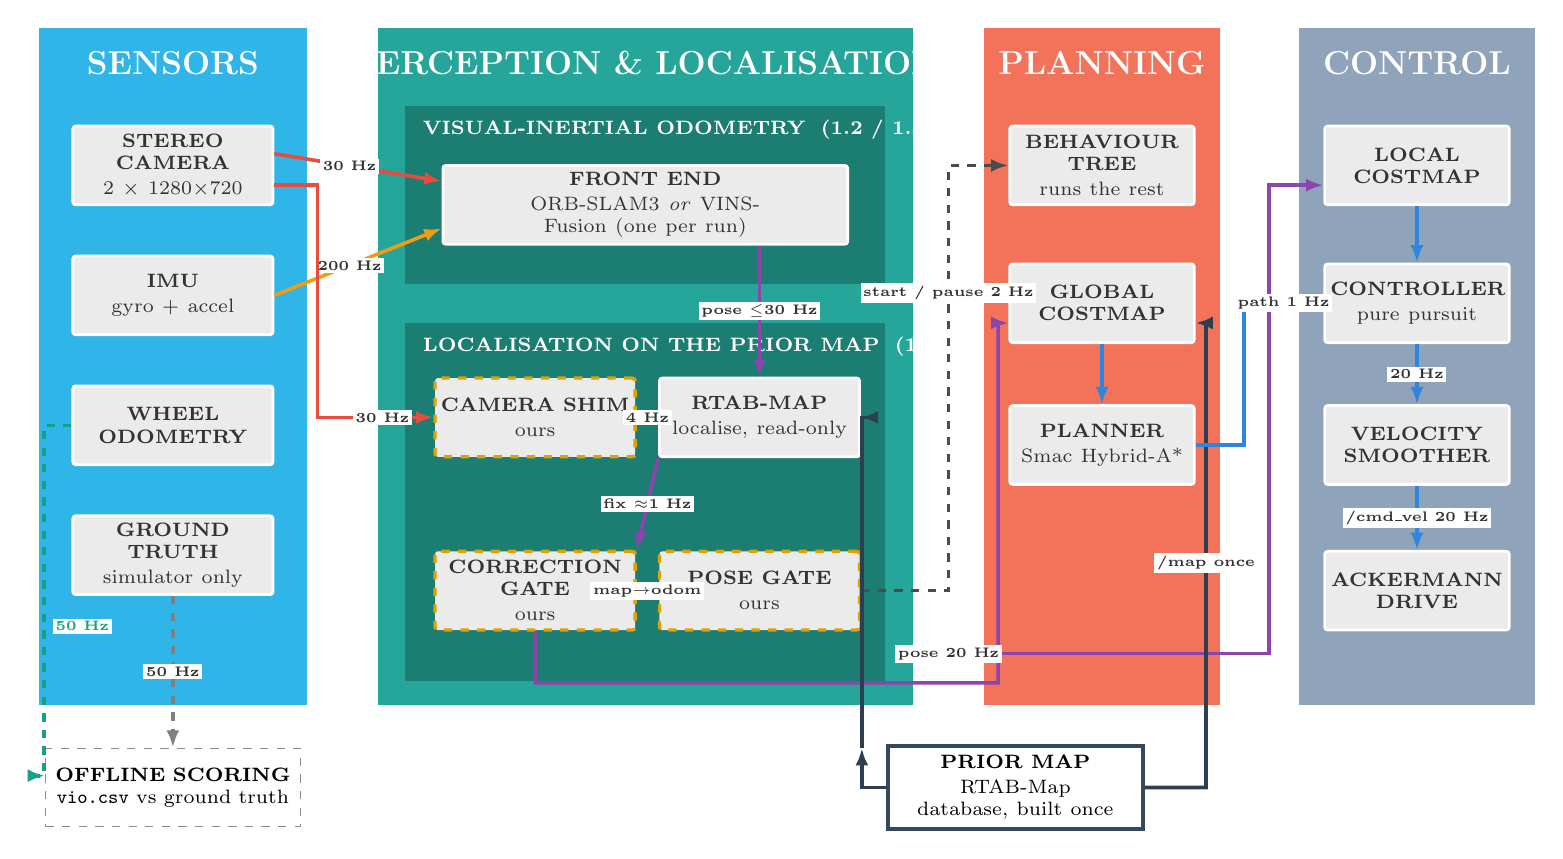
\begin{tikzpicture}[font=\footnotesize,
      ib/.style={draw=white, line width=1pt, rounded corners=1pt, align=center,
                 font=\scriptsize\bfseries, text=black!80, fill=white!92!black,
                 text width=24mm, minimum height=10mm, inner sep=2pt},
      hdr/.style={font=\large\bfseries, text=white},
      dl/.style={-{Latex[length=2.2mm]}, line width=1.3pt},
      rt/.style={font=\tiny\bfseries, fill=white, inner sep=1pt, text=black!80}]
    % ---------------- column panels
    \fill[sensorcol] (0,-4.4) rectangle (3.4,4.2);
    \node[hdr] at (1.7,3.75) {SENSORS};
    \fill[perccol] (4.3,-4.4) rectangle (11.1,4.2);
    \node[hdr] at (7.7,3.75) {PERCEPTION \& LOCALISATION};
    \fill[plancol] (12.0,-4.4) rectangle (15.0,4.2);
    \node[hdr] at (13.5,3.75) {PLANNING};
    \fill[ctrlcol] (16.0,-4.4) rectangle (19.0,4.2);
    \node[hdr] at (17.5,3.75) {CONTROL};
    % sub-panels inside perception
    \fill[black!25!perccol] (4.65,0.95) rectangle (10.75,3.2);
    \node[font=\scriptsize\bfseries, text=white, anchor=north west] at (4.75,3.15)
      {VISUAL-INERTIAL ODOMETRY \;(1.2 / 1.3)};
    \fill[black!25!perccol] (4.65,-4.1) rectangle (10.75,0.45);
    \node[font=\scriptsize\bfseries, text=white, anchor=north west] at (4.75,0.4)
      {LOCALISATION ON THE PRIOR MAP \;(1.4)};
    % ---------------- boxes
    \node[ib] at (1.7, 2.45) (cam) {STEREO CAMERA\\[1pt]\mdseries 2 $\times$ 1280$\times$720};
    \node[ib] at (1.7, 0.80) (imu) {IMU\\[1pt]\mdseries gyro + accel};
    \node[ib] at (1.7,-0.85) (whl) {WHEEL ODOMETRY};
    \node[ib] at (1.7,-2.50) (gt)  {GROUND TRUTH\\[1pt]\mdseries simulator only};
    \node[ib, text width=50mm] at (7.7, 1.95) (fe)
      {FRONT END\\[1pt]\mdseries ORB-SLAM3 \emph{or} VINS-Fusion (one per run)};
    \node[ib, ours] at (6.3,-0.75) (shim) {CAMERA SHIM\\[1pt]\mdseries ours};
    \node[ib]       at (9.15,-0.75) (rtab) {RTAB-MAP\\[1pt]\mdseries localise, read-only};
    \node[ib, ours] at (6.3,-2.95) (cg) {CORRECTION GATE\\[1pt]\mdseries ours};
    \node[ib, ours] at (9.15,-2.95) (pg) {POSE GATE\\[1pt]\mdseries ours};
    \node[ib, text width=22mm] at (13.5, 2.45) (bt)  {BEHAVIOUR TREE\\[1pt]\mdseries runs the rest};
    \node[ib, text width=22mm] at (13.5, 0.70) (gcm) {GLOBAL COSTMAP};
    \node[ib, text width=22mm] at (13.5,-1.10) (pl)  {PLANNER\\[1pt]\mdseries Smac Hybrid-A*};
    \node[ib, text width=22mm] at (17.5, 2.45) (lcm) {LOCAL COSTMAP};
    \node[ib, text width=22mm] at (17.5, 0.70) (ct)  {CONTROLLER\\[1pt]\mdseries pure pursuit};
    \node[ib, text width=22mm] at (17.5,-1.10) (sm)  {VELOCITY\\SMOOTHER};
    \node[ib, text width=22mm] at (17.5,-2.95) (drv) {ACKERMANN\\DRIVE};
    % MAP and SCORING, under the panels as in the reference
    \node[draw=mapcol, line width=1.3pt, fill=white, font=\scriptsize\bfseries,
          align=center, text width=30mm, minimum height=10mm] at (12.4,-5.45) (map)
      {PRIOR MAP\\[1pt]\mdseries RTAB-Map database, built once};
    \node[draw=black!45, dashed, fill=white, font=\scriptsize, align=center,
          text width=30mm, minimum height=10mm] at (1.7,-5.45) (eval)
      {\textbf{OFFLINE SCORING}\\ \repo{vio.csv} vs ground truth};
    % ---------------- data lines (colour = kind of data)
    \draw[dl, dimg] ($(cam.east)+(0,0.15)$) -- node[rt, pos=0.45]{30 Hz} ($(fe.west)+(0,0.30)$);
    \draw[dl, dimu] (imu.east) -- node[rt, pos=0.45]{200 Hz} ($(fe.west)+(0,-0.30)$);
    \draw[dl, dimg] ($(cam.east)+(0,-0.25)$) -- ++(0.55,0) |- node[rt, pos=0.78]{30 Hz} (shim.west);
    \draw[dl, dimg] (shim.east) -- node[rt]{4 Hz} (rtab.west);
    \draw[dl, dpose] (fe.south -| rtab.north) -- node[rt]{pose $\le$30 Hz} (rtab.north);
    \draw[dl, dpose] (rtab.south west) -- node[rt, pos=0.5]{fix $\approx$1 Hz} (cg.north east);
    \draw[dl, dpose] (cg.east) -- node[rt]{map$\rightarrow$odom} (pg.west);
    % the robot's pose reaches planning and control through TF
    \draw[dl, dpose] (cg.south) -- ++(0,-0.65) -| (12.18,0.45) -- ($(gcm.west)+(0,-0.25)$);
    \draw[dl, dpose] (12.18,-3.75) -| (15.62,2.2) -- ($(lcm.west)+(0,-0.25)$);
    \node[rt] at (11.55,-3.75) {pose 20 Hz};
    % gate decides whether Nav2 runs at all
    \draw[dl, black!70, dashed] (pg.east) -- (11.55,-2.95) |- node[rt, pos=0.35]{start / pause 2 Hz} (bt.west);
    % the map
    \draw[dl, dmap] (10.45,-4.95) |- (rtab.east);
    \draw[dl, dmap] (map.west) -- (10.45,-5.45) -- (10.45,-4.95);
    \draw[dl, dmap] (map.east) -| (14.82,0.45) -- ($(gcm.east)+(0,-0.25)$);
    \node[rt] at (14.82,-2.6) {/map once};
    % planning -> control
    \draw[dl, dcmd] (gcm) -- (pl);
    \draw[dl, dcmd] (pl.east) -- (15.3,-1.10) |- node[rt, pos=0.75]{path 1 Hz} (ct.west);
    \draw[dl, dcmd] (lcm) -- (ct);
    \draw[dl, dcmd] (ct) -- node[rt]{20 Hz} (sm);
    \draw[dl, dcmd] (sm) -- node[rt]{/cmd\_vel 20 Hz} (drv);
    % offline
    \draw[dl, dwhl, dashed] (whl.west) -- ++(-0.35,0) |- ($(eval.west)+(0,0.15)$);
    \draw[dl, black!50, dashed] (gt.south) -- node[rt]{50 Hz} (eval.north);
    \node[rt, text=dwhl] at (0.55,-3.4) {50 Hz};
  \end{tikzpicture}}
  \par\vspace{0.2em}
  \scriptsize\color{black!70}
  Line colour = kind of data:
  \textcolor{dimg}{\textbf{images}} \textperiodcentered\
  \textcolor{dimu}{\textbf{IMU}} \textperiodcentered\
  \textcolor{dpose}{\textbf{robot pose}} \textperiodcentered\
  \textcolor{dmap}{\textbf{map}} \textperiodcentered\
  \textcolor{dcmd}{\textbf{path and commands}} \textperiodcentered\
  \textcolor{dwhl}{\textbf{wheels}}.
  \quad Dashed amber box = written for this project.
  \quad Real rig: same graph; fisheye cameras, optical-tracker ground truth.
\end{frame}

% -----------------------------------------------------------------------------
\begin{frame}{1.1 \;Three clocks: the system runs at three different speeds, on purpose}
  \begin{columns}[T]
    \column{0.60\textwidth}
      \centering
      \adjustbox{max width=\linewidth}{%
      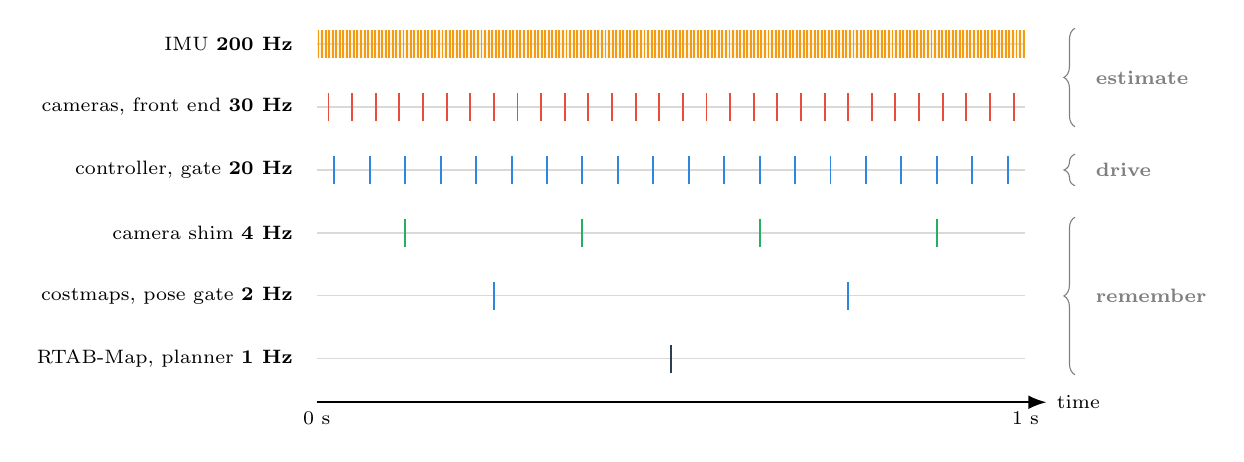
\begin{tikzpicture}[x=9cm, font=\scriptsize]
        \fill[dimu!10] (0,4.82) rectangle (1,5.18);
        \lane{5.0}{IMU \textbf{200 Hz}}{200}{dimu}
        \lane{4.2}{cameras, front end \textbf{30 Hz}}{30}{dimg}
        \lane{3.4}{controller, gate \textbf{20 Hz}}{20}{dcmd}
        \lane{2.6}{camera shim \textbf{4 Hz}}{4}{rtabc}
        \lane{1.8}{costmaps, pose gate \textbf{2 Hz}}{2}{navc}
        \lane{1.0}{RTAB-Map, planner \textbf{1 Hz}}{1}{dmap}
        \draw[thick, -{Latex}] (0,0.45) -- (1.03,0.45) node[right]{time};
        \node[below] at (0,0.45) {0 s}; \node[below] at (1,0.45) {1 s};
        \draw[decorate, decoration={brace, amplitude=4pt, mirror}, black!50]
          (1.07,5.2) -- node[right=4pt, align=left]{\textbf{estimate}} (1.07,3.95);
        \draw[decorate, decoration={brace, amplitude=4pt, mirror}, black!50]
          (1.07,3.6) -- node[right=4pt, align=left]{\textbf{drive}} (1.07,3.2);
        \draw[decorate, decoration={brace, amplitude=4pt, mirror}, black!50]
          (1.07,2.8) -- node[right=4pt, align=left]{\textbf{remember}} (1.07,0.8);
      \end{tikzpicture}}
      \par{\scriptsize One second of the system. Each tick is one update.}
    \column{0.38\textwidth}
      \small
      \textbf{\color{dimg}Estimate, fast.} The front end must follow every
      camera frame and IMU sample, or frames are dropped.
      \par\vspace{0.6em}
      \textbf{\color{dcmd}Drive, steady.} The controller corrects the steering
      20 times a second.
      \par\vspace{0.6em}
      \textbf{\color{dmap}Remember, slow.} Recognising a place is expensive and
      places do not change quickly, so RTAB-Map looks once a second.
      \par\vspace{0.8em}
      \scriptsize\color{black!65}
      Consequence: a slow correction lands on top of a fast estimate. The next
      slide shows how the two are stacked.
  \end{columns}
\end{frame}

% -----------------------------------------------------------------------------
\begin{frame}{1.1 \;The frame chain: two answers to ``where is the robot?'', stacked}
  \begin{columns}[T]
    \column{0.52\textwidth}
      \centering
      \adjustbox{max width=\linewidth, max height=0.78\textheight}{%
      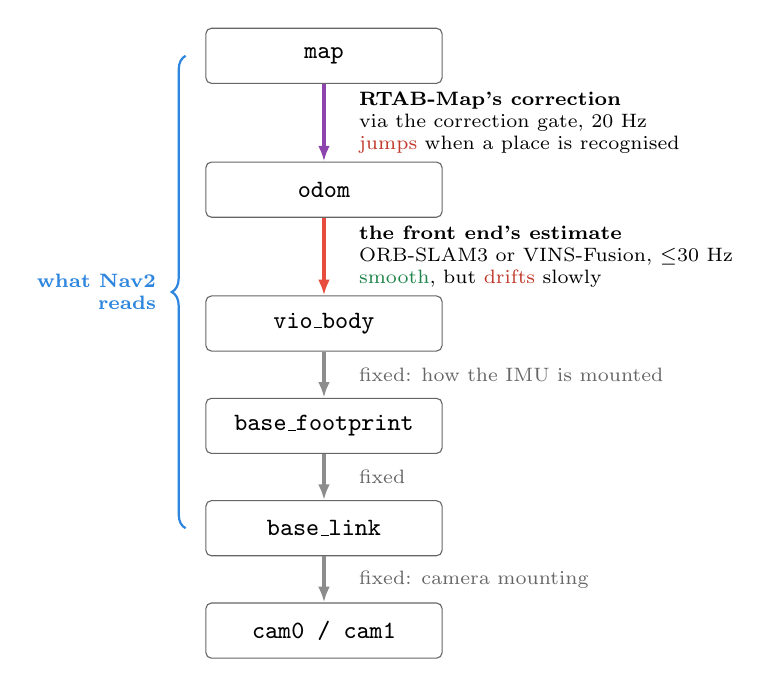
\begin{tikzpicture}[font=\scriptsize,
          fr/.style={draw=black!60, fill=white, rounded corners=2pt,
                     font=\small\ttfamily, minimum width=30mm, minimum height=7mm},
          lk/.style={-{Latex[length=2mm]}, line width=1.6pt}]
        \node[fr] (map) at (0,0)    {map};
        \node[fr] (odo) at (0,-1.7) {odom};
        \node[fr] (vio) at (0,-3.4) {vio\_body};
        \node[fr] (bfp) at (0,-4.7) {base\_footprint};
        \node[fr] (bl)  at (0,-6.0) {base\_link};
        \node[fr] (cm)  at (0,-7.3) {cam0 / cam1};
        \draw[lk, dpose] (map) -- node[right=3mm, align=left, text=black]
          {\textbf{RTAB-Map's correction}\\via the correction gate, 20 Hz\\
           \textcolor{bad}{jumps} when a place is recognised} (odo);
        \draw[lk, dimg] (odo) -- node[right=3mm, align=left, text=black]
          {\textbf{the front end's estimate}\\ORB-SLAM3 or VINS-Fusion, $\le$30 Hz\\
           \textcolor{good}{smooth}, but \textcolor{bad}{drifts} slowly} (vio);
        \draw[lk, black!45] (vio) -- node[right=3mm, text=black!60]{fixed: how the IMU is mounted} (bfp);
        \draw[lk, black!45] (bfp) -- node[right=3mm, text=black!60]{fixed} (bl);
        \draw[lk, black!45] (bl) -- node[right=3mm, text=black!60]{fixed: camera mounting} (cm);
        \draw[decorate, decoration={brace, amplitude=5pt, mirror}, thick, navc]
          ($(map.west)+(-0.25,0)$) -- node[left=7pt, align=right, text=navc]
          {\textbf{what Nav2}\\\textbf{reads}} ($(bl.west)+(-0.25,0)$);
      \end{tikzpicture}}
    \column{0.46\textwidth}
      \small
      \textbf{Why two links instead of one?}
      \par\vspace{0.3em}
      The front end is like a \textbf{watch}: it ticks smoothly every frame, but
      slowly runs fast or slow.
      \par\vspace{0.3em}
      RTAB-Map is like a \textbf{church clock}: right, but you only see it now
      and then.
      \par\vspace{0.3em}
      You keep reading the watch, and reset it whenever you see the clock.
      \texttt{map}$\rightarrow$\texttt{odom} is that reset.
      \par\vspace{0.8em}
      \scriptsize\color{black!65}
      So the pose Nav2 uses is \emph{watch} $+$ \emph{latest reset}: it moves
      smoothly between fixes, and steps when a fix arrives.
  \end{columns}
\end{frame}

% =============================================================================
% 1.2  ORB-SLAM3
% Sources: Campos et al., ORB-SLAM3, IEEE T-RO 2021 (Fig. 1, sections III, V, VI)
% and orbslam3_ros2/config/wil_sim/stereo_imu.yaml, config/wil/stereo_imu.yaml.
% Signal columns are the headers of the CSVs every run writes.
% =============================================================================
\section{1.2 ORB-SLAM3}

\begin{frame}{1.2 \;ORB-SLAM3: three threads share one map}
  \centering
  \adjustbox{max width=\textwidth, max height=0.70\textheight}{%
  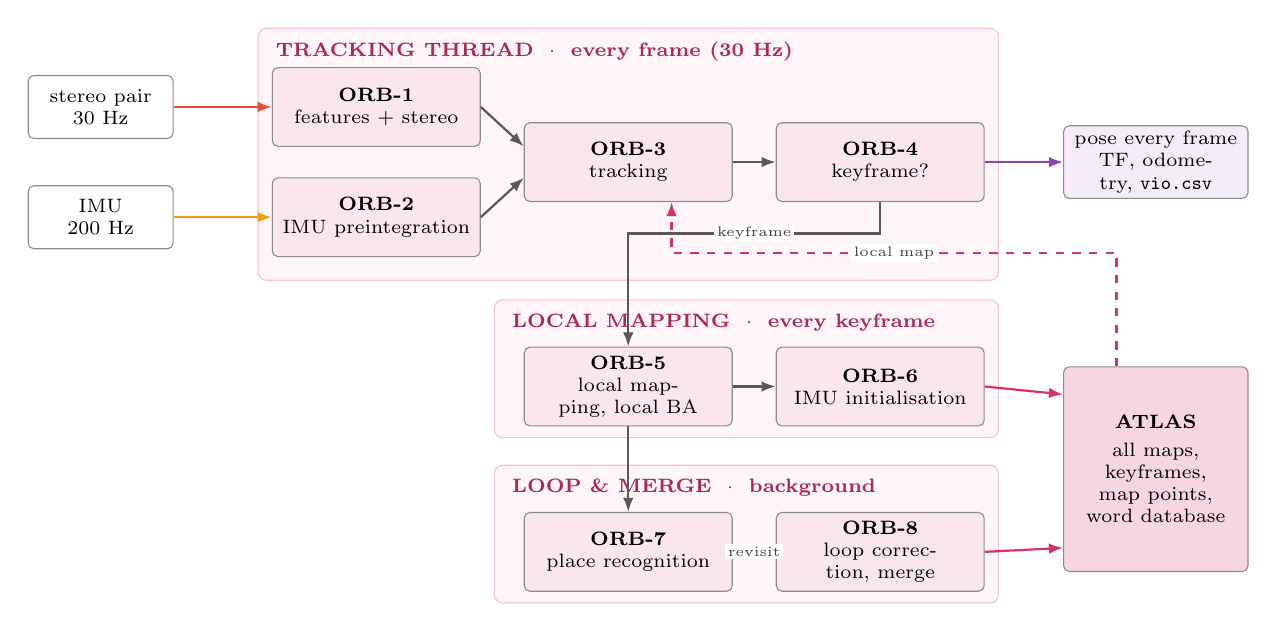
\begin{tikzpicture}[font=\scriptsize,
      cb/.style={box, fill=orbc!12, text width=25mm, minimum height=10mm},
      band/.style={fill=orbc!5, draw=orbc!30, rounded corners=3pt},
      bl/.style={font=\scriptsize\bfseries, text=orbc!80!black, anchor=north west}]
    % thread bands
    \fill[band] (2.0,-1.75) rectangle (11.4,1.45);
    \node[bl] at (2.1,1.4) {TRACKING THREAD \;$\cdot$\; every frame (30 Hz)};
    \fill[band] (5.0,-3.75) rectangle (11.4,-2.0);
    \node[bl] at (5.1,-2.05) {LOCAL MAPPING \;$\cdot$\; every keyframe};
    \fill[band] (5.0,-5.85) rectangle (11.4,-4.1);
    \node[bl] at (5.1,-4.15) {LOOP \& MERGE \;$\cdot$\; background};
    % inputs
    \node[box, text width=17mm] (st) at (0,0.45) {stereo pair\\30 Hz};
    \node[box, text width=17mm] (im) at (0,-0.95) {IMU\\200 Hz};
    % components
    \node[cb, ORB1] (o1) at (3.5,0.45)  {\textbf{ORB-1}\\features + stereo};
    \node[cb, ORB2] (o2) at (3.5,-0.95) {\textbf{ORB-2}\\IMU preintegration};
    \node[cb, ORB3] (o3) at (6.7,-0.25) {\textbf{ORB-3}\\tracking};
    \node[cb, ORB4] (o4) at (9.9,-0.25) {\textbf{ORB-4}\\keyframe?};
    \node[cb, ORB5] (o5) at (6.7,-3.1)  {\textbf{ORB-5}\\local mapping, local BA};
    \node[cb, ORB6] (o6) at (9.9,-3.1)  {\textbf{ORB-6}\\IMU initialisation};
    \node[cb, ORB7] (o7) at (6.7,-5.2)  {\textbf{ORB-7}\\place recognition};
    \node[cb, ORB8] (o8) at (9.9,-5.2)  {\textbf{ORB-8}\\loop correction, merge};
    % outputs and the map store
    \node[box, text width=22mm, fill=dpose!10] (out) at (13.4,-0.25)
      {pose every frame\\TF, odometry, \repo{vio.csv}};
    \node[box, text width=22mm, minimum height=26mm, fill=orbc!20] (atl) at (13.4,-4.15)
      {\textbf{ATLAS}\\[2pt]all maps,\\keyframes,\\map points,\\word database};
    % flow
    \draw[arr, dimg] (st) -- (o1);
    \draw[arr, dimu] (im) -- (o2);
    \draw[arr] (o1.east) -- ($(o3.west)+(0,0.2)$);
    \draw[arr] (o2.east) -- ($(o3.west)+(0,-0.2)$);
    \draw[arr] (o3) -- (o4);
    \draw[arr, dpose] (o4.east) -- (out.west);
    \draw[arr] (o4.south) -- ++(0,-0.4) -| node[rate, pos=0.25]{keyframe} (o5.north);
    \draw[arr] (o5) -- (o6);
    \draw[arr] (o5) -- (o7);
    \draw[arr] (o7) -- node[rate]{revisit} (o8);
    \draw[arr, orbc] (o6.east) -- ($(atl.west)+(0,0.95)$);
    \draw[arr, orbc] (o8.east) -- ($(atl.west)+(0,-1.0)$);
    \draw[darr, orbc] ($(atl.north)+(-0.5,0)$) |- node[rate, pos=0.75]{local map} (7.25,-1.4) -- ($(o3.south)+(0.55,0)$);
  \end{tikzpicture}}
  \par\vspace{0.3em}
  \small Three threads run side by side and share one store of maps, the
  \textbf{Atlas}. Tracking must keep up with the camera; the other two take as
  long as they need without holding it back.
  \src{After Campos et al., ORB-SLAM3, IEEE T-RO 2021, Fig.~1.}
\end{frame}

% ---------------------------------------------------------------- ORB-1
\begin{frame}{1.2.1 \;ORB-1 \;Features: turn an image into points you can find again}
  \hl{ORB1}\res{\R{1}{}, \R{8}{}, \R{9}{}}
  \compbody{\orbstrip}{orbc}{%
  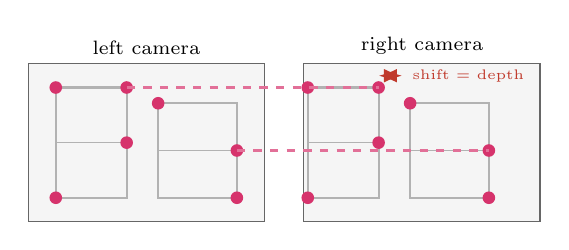
\begin{tikzpicture}[font=\scriptsize]
    \foreach \ox/\lbl/\sh in {0/left camera/0, 3.5/right camera/-0.3} {
      \draw[black!60, fill=black!4] (\ox,0) rectangle ++(3,2);
      \node[above] at (\ox+1.5,2) {\lbl};
      \draw[black!30, thick] (\ox+0.35+\sh,0.3) rectangle ++(0.9,1.4);
      \draw[black!30, thick] (\ox+1.65+\sh,0.3) rectangle ++(1.0,1.2);
      \draw[black!30] (\ox+0.35+\sh,1.0) -- ++(0.9,0);
      \draw[black!30] (\ox+1.65+\sh,0.9) -- ++(1.0,0);
    }
    \foreach \x/\y in {0.35/0.3, 1.25/1.7, 1.25/1.0, 1.65/1.5, 2.65/0.3, 2.65/0.9, 0.35/1.7} {
      \node[pt=orbc] at (\x,\y) {};
      \node[pt=orbc] at (3.5+\x-0.3,\y) {};
    }
    \foreach \x/\y in {1.25/1.7, 2.65/0.9}
      \draw[orbc!70, dashed, thick] (\x,\y) -- (3.5+\x-0.3,\y);
    \draw[{Latex}-{Latex}, hlc, thick] (3.5+1.25-0.3,1.85) -- (3.5+1.25,1.85)
      node[right, font=\tiny, text=hlc]{shift = depth};
  \end{tikzpicture}}%
  {Corners are found at 8 image sizes, each gets a 256-bit fingerprint, and the
   left--right shift of a matched pair gives its distance.}
  {A camera image is a million pixels. The system needs a few hundred
   distinctive points it can find again in the next frame, and later.}
  {stereo pair, 30 Hz}
  {$\approx$1\,500 points with fingerprints, most with depth}
  {Blank walls give few corners. Extraction slower than 33\,ms drops frames.}
  {\repo{tracking_frontend.csv}: features, extraction time;
   \repo{performance.csv}: frames received vs processed}
  \src{GPU extractor in simulation is our fork's patch~10; the real rig runs the CPU one.}
\end{frame}

% ---------------------------------------------------------------- ORB-1 inside
% How ORB itself works, after "image copy 2.png" (four stages). Values checked
% against thirdparty/ORB_SLAM3/src: FAST(..., iniThFAST, true) = OpenCV FAST-9/16,
% IC_Angle over HALF_PATCH_SIZE 15 (31 px patch), ORBmatcher TH_LOW 50 /
% TH_HIGH 100, cells W = 35 px.  The Hamming example is computed, not copied.
\begin{frame}{1.2.1 \;ORB-1 \;Inside: how ORB turns pixels into a point you can match}
  \hl{ORB1}\res{\R{1}{}, \R{8}{}, \R{9}{}}
  \orbstrip\par\vspace{0.3em}
  \centering
  \adjustbox{max width=\textwidth, max height=0.66\textheight}{%
  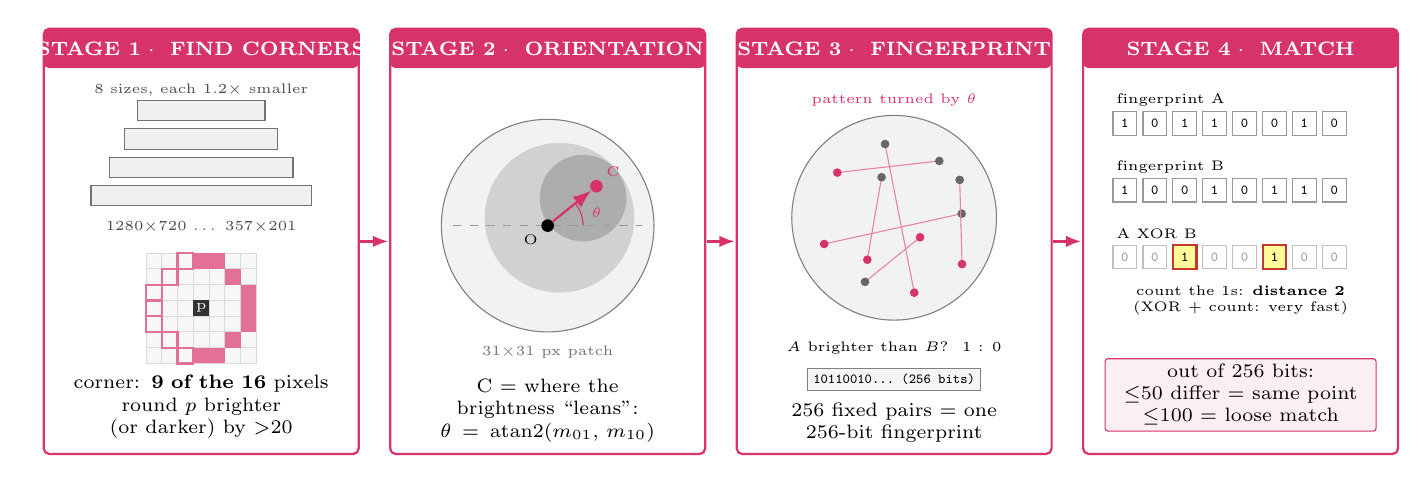
\begin{tikzpicture}[font=\scriptsize,
      capt/.style={align=center, text width=35mm, font=\scriptsize},
      tag/.style={draw=orbc, fill=orbc!8, rounded corners=1pt, font=\tiny, inner sep=2pt}]
    % ---- four panels with headers
    \foreach \i/\x/\t in {1/0/FIND CORNERS, 2/4.4/ORIENTATION, 3/8.8/FINGERPRINT, 4/13.2/MATCH} {
      \draw[orbc, line width=0.8pt, rounded corners=2pt, fill=white] (\x,0) rectangle ++(4.0,5.4);
      \fill[orbc, rounded corners=2pt] (\x,4.9) rectangle ++(4.0,0.5);
      \node[text=white, font=\scriptsize\bfseries] at (\x+2.0,5.15) {STAGE \i \;$\cdot$\; \t};}
    \foreach \x in {4.0,8.4,12.8} \draw[-{Latex[length=2mm]}, very thick, orbc] (\x+0.02,2.7) -- (\x+0.38,2.7);
    % ---- STAGE 1: pyramid
    \foreach \k/\w in {0/2.8, 1/2.33, 2/1.94, 3/1.62}
      \draw[black!55, fill=black!6] ({2.0-\w/2},{3.15+\k*0.36}) rectangle ++(\w,0.26);
    \node[font=\tiny, text=black!70] at (2.0,4.62) {8 sizes, each 1.2$\times$ smaller};
    \node[font=\tiny, text=black!70] at (2.0,2.88) {1280$\times$720 \ldots\ 357$\times$201};
    % ---- STAGE 1: FAST circle (Bresenham radius 3, 16 pixels; 9 in a row brighter)
    \begin{scope}[shift={(2.0,1.85)}]
      \foreach \u in {-3,...,3} \foreach \v in {-3,...,3}
        \draw[black!15, fill=black!3] (\u*0.2-0.1,\v*0.2-0.1) rectangle ++(0.2,0.2);
      \foreach [count=\n] \u/\v in {0/3,1/3,2/2,3/1,3/0,3/-1,2/-2,1/-3,0/-3,-1/-3,-2/-2,-3/-1,-3/0,-3/1,-2/2,-1/3} {
        \ifnum\n<10 \fill[orbc!70] (\u*0.2-0.1,\v*0.2-0.1) rectangle ++(0.2,0.2);
        \else       \draw[orbc!70, thick] (\u*0.2-0.1,\v*0.2-0.1) rectangle ++(0.2,0.2); \fi}
      \fill[black!80] (-0.1,-0.1) rectangle ++(0.2,0.2);
      \node[font=\tiny, text=white] at (0,0) {p};
    \end{scope}
    \node[capt] at (2.0,0.6) {corner: \textbf{9 of the 16} pixels\\round $p$ brighter (or darker) by $>$20};
    % ---- STAGE 2: orientation by intensity centroid
    \begin{scope}[shift={(6.4,2.9)}]
      \fill[black!5] (0,0) circle (1.35);
      \fill[black!18] (0.15,0.1) circle (0.95);
      \fill[black!32] (0.45,0.35) circle (0.55);
      \draw[black!50] (0,0) circle (1.35);
      \draw[black!40, dashed] (-1.2,0) -- (1.2,0);
      \node[pt=black] (O) at (0,0) {}; \node[below left, font=\tiny] at (O) {O};
      \node[pt=orbc] (C) at (0.62,0.5) {}; \node[above right, font=\tiny, text=orbc] at (C) {C};
      \draw[-{Latex}, thick, orbc] (O) -- (C);
      \draw[orbc] (0.45,0) arc (0:39:0.45); \node[font=\tiny, text=orbc] at (0.62,0.17) {$\theta$};
      \node[font=\tiny, text=black!55] at (0,-1.6) {31$\times$31 px patch};
    \end{scope}
    \node[capt] at (6.4,0.55) {C = where the brightness ``leans'':\\$\theta = \mathrm{atan2}(m_{01},\, m_{10})$};
    % ---- STAGE 3: rotated BRIEF
    \begin{scope}[shift={(10.8,3.0)}]
      \fill[black!5] (0,0) circle (1.3); \draw[black!50] (0,0) circle (1.3);
      \begin{scope}[rotate=39]
        \foreach \a/\b/\c/\d in {-0.9/0.3/0.7/-0.5, -0.4/-0.9/0.5/0.8, -0.2/0.9/0.9/0.2,
                                 0.1/-0.4/-0.8/-0.4, -0.6/-0.2/0.2/0.5, 0.3/-1.0/0.95/-0.15} {
          \draw[orbc!60] (\a,\b) -- (\c,\d);
          \node[pt=orbc, minimum size=1.1mm] at (\a,\b) {}; \node[pt=black!60, minimum size=1.1mm] at (\c,\d) {};}
      \end{scope}
      \node[font=\tiny, text=orbc] at (0,1.5) {pattern turned by $\theta$};
    \end{scope}
    \node[font=\tiny] at (10.8,1.35) {$A$ brighter than $B$? \;1 : 0};
    \node[draw=black!50, fill=black!4, font=\tiny\ttfamily, inner sep=2pt] at (10.8,0.95) {10110010\ldots\ (256 bits)};
    \node[capt] at (10.8,0.4) {256 fixed pairs = one 256-bit fingerprint};
    % ---- STAGE 4: Hamming distance (computed example)
    \begin{scope}[shift={(13.55,4.2)}, font=\tiny\ttfamily]
      \node[anchor=west, font=\tiny] at (-0.05,0.3) {fingerprint A};
      \node[anchor=west, font=\tiny] at (-0.05,-0.55) {fingerprint B};
      \node[anchor=west, font=\tiny] at (-0.05,-1.4) {A XOR B};
      \foreach [count=\n] \a/\b in {1/1,0/0,1/0,1/1,0/0,0/1,1/1,0/0} {
        \pgfmathtruncatemacro{\x}{\a==\b ? 0 : 1}
        \node[draw=black!40, minimum size=3mm, inner sep=0pt] at (\n*0.38-0.2,0.0) {\a};
        \node[draw=black!40, minimum size=3mm, inner sep=0pt] at (\n*0.38-0.2,-0.85) {\b};
        \ifnum\x=1
          \node[draw=hlc, fill=yellow!40, thick, minimum size=3mm, inner sep=0pt] at (\n*0.38-0.2,-1.7) {1};
        \else
          \node[draw=black!25, minimum size=3mm, inner sep=0pt, text=black!40] at (\n*0.38-0.2,-1.7) {0};
        \fi}
    \end{scope}
    \node[font=\tiny, align=center] at (15.2,1.95) {count the 1s: \textbf{distance 2}\\(XOR + count: very fast)};
    \node[tag, align=center, text width=33mm, font=\scriptsize] at (15.2,0.75) {out of 256 bits:\\$\le$50 differ = same point\\$\le$100 = loose match};
  \end{tikzpicture}}
  \par\vspace{0.15em}
  \scriptsize\color{black!70}
  ORB-SLAM3 adds one step to stage~1: the image is cut into 35$\times$35 px cells so the 1\,500 points
  spread over the whole frame, and a dull cell retries with a lower threshold (7 instead of 20).
  \src{Rublee et al., ORB, ICCV 2011; checked against \repo{thirdparty/ORB_SLAM3/src/ORBextractor.cc}, \repo{ORBmatcher.cc}.}
\end{frame}

% ---------------------------------------------------------------- ORB-2
\begin{frame}{1.2.2 \;ORB-2 \;IMU preintegration: summarise the readings between two frames}
  \hl{ORB2}\res{\R{5}{}, \R{8}{}}
  \compbody{\orbstrip}{orbc}{%
  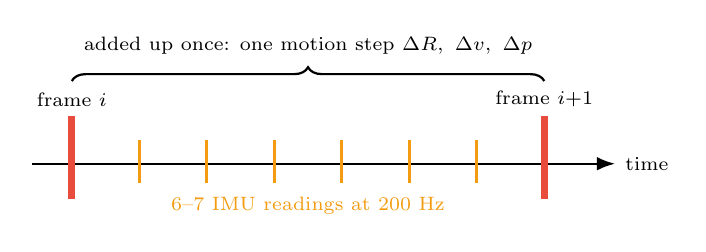
\begin{tikzpicture}[font=\scriptsize]
    \draw[thick,-{Latex}] (0,0) -- (7.4,0) node[right]{time};
    \foreach \x/\l in {0.5/frame $i$, 6.5/frame $i{+}1$} {
      \draw[line width=2.4pt, dimg] (\x,-0.45) -- (\x,0.6);
      \node[above] at (\x,0.6) {\l};}
    \foreach \k in {1,...,6} \draw[dimu, line width=1.2pt]
      ({0.5+\k*6/7},-0.25) -- ({0.5+\k*6/7},0.3);
    \node[below, text=dimu] at (3.5,-0.3) {6--7 IMU readings at 200 Hz};
    \draw[decorate, decoration={brace, amplitude=5pt}, thick]
      (0.5,1.05) -- node[above=6pt]{added up once: one motion step $\Delta R,\ \Delta v,\ \Delta p$} (6.5,1.05);
  \end{tikzpicture}}%
  {Rotation, velocity and position change between the frames, with an
   uncertainty built from the IMU noise values in the config.}
  {The IMU reports about 7 times between two frames. Adding them up once,
   instead of at every optimiser step, keeps everything fast.}
  {IMU, 200 Hz}
  {one motion step + uncertainty per frame pair}
  {Wrong noise values make the IMU over- or under-trusted. Missing samples leave a gap.}
  {\repo{performance.csv}: imu\_samples, imu\_starved;
   \repo{tracking_frontend.csv}: preintegration time}
\end{frame}

% ---------------------------------------------------------------- ORB-3
\begin{frame}{1.2.3 \;ORB-3 \;Tracking: where is the camera, right now?}
  \hl{ORB3}\res{\R{5}{}, \R{7}{}}
  \compbody{\orbstrip}{orbc}{%
  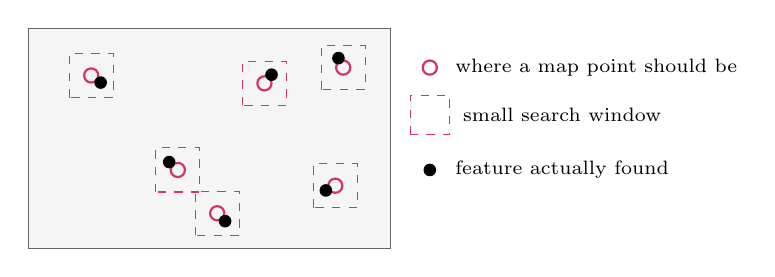
\begin{tikzpicture}[font=\scriptsize]
    \draw[black!60, fill=black!4] (0,0) rectangle (4.6,2.8);
    \foreach \x/\y/\dx/\dy in {0.8/2.2/0.12/-0.09, 1.9/1.0/-0.11/0.1, 3.0/2.1/0.09/0.11,
                               3.9/0.8/-0.12/-0.06, 2.4/0.45/0.1/-0.1, 4.0/2.3/-0.06/0.12} {
      \draw[orbc, dashed] (\x-0.28,\y-0.28) rectangle (\x+0.28,\y+0.28);
      \draw[orbc, thick] (\x,\y) circle (0.09);
      \node[pt=black] at (\x+\dx,\y+\dy) {};}
    \draw[orbc, thick] (5.1,2.3) circle (0.09); \node[anchor=west] at (5.3,2.3) {where a map point should be};
    \draw[orbc, dashed] (4.85,1.45) rectangle ++(0.5,0.5); \node[anchor=west] at (5.4,1.7) {small search window};
    \node[pt=black] at (5.1,1.0) {}; \node[anchor=west] at (5.3,1.0) {feature actually found};
  \end{tikzpicture}}%
  {\textcircled{\tiny 1} predict the pose from the IMU \textcircled{\tiny 2} look for each
   map point near where it should be \textcircled{\tiny 3} nudge the pose until they line up.}
  {Every frame needs a pose now; the robot cannot wait for the map to be refined.}
  {points (ORB-1), IMU step (ORB-2), local map}
  {pose every frame $\rightarrow$ TF, odometry, \repo{vio.csv}}
  {Fewer than 15 matches and tracking is lost. One slow frame delays all after it.}
  {\repo{performance.csv}: tracking\_state, tracking\_ms;
   \repo{tracking_frontend.csv}: map\_matches\_inliers}
\end{frame}

% ---------------------------------------------------------------- ORB-4
\begin{frame}{1.2.4 \;ORB-4 \;Keyframe decision: which frames are worth remembering?}
  \hl{ORB4}
  \compbody{\orbstrip}{orbc}{%
  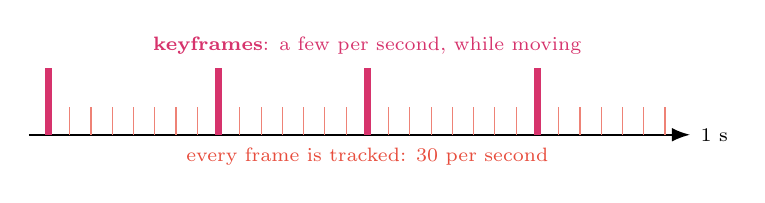
\begin{tikzpicture}[font=\scriptsize]
    \draw[thick,-{Latex}] (0,0) -- (8.4,0) node[right]{1 s};
    \foreach \k in {0,...,29} \draw[dimg!70] ({0.25+\k*0.27},0) -- ++(0,0.35);
    \foreach \k in {0,8,15,23} \draw[orbc, line width=2.4pt] ({0.25+\k*0.27},0) -- ++(0,0.85);
    \node[above, text=orbc] at (4.3,0.9) {\textbf{keyframes}: a few per second, while moving};
    \node[below, text=dimg] at (4.3,-0.05) {every frame is tracked: 30 per second};
  \end{tikzpicture}}%
  {A frame becomes a keyframe when it sees enough that the last keyframe did
   not, or too long has passed since the last one.}
  {Keeping all 30 frames a second would fill the map with near-copies. The map
   is built from keyframes only.}
  {each tracked frame}
  {a keyframe, a few times per second}
  {Too many and the mapping queue backs up; too few and the map has gaps.}
  {\repo{tracking_frontend.csv}: keyframes\_created;
   one row per keyframe in \repo{local_mapping.csv}}
\end{frame}

% ---------------------------------------------------------------- ORB-5
\begin{frame}{1.2.5 \;ORB-5 \;Local mapping: refine the recent part of the map}
  \hl{ORB5}\res{\R{9}{}}
  \compbody{\orbstrip}{orbc}{%
  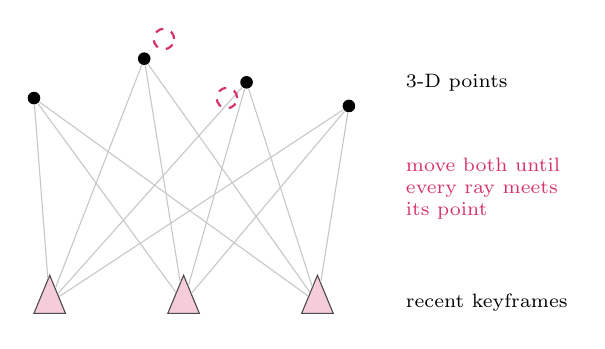
\begin{tikzpicture}[font=\scriptsize]
    \foreach \i/\x in {1/0.5,2/2.2,3/3.9} \node[cam=90, fill=orbc!25] (k\i) at (\x,0) {};
    \foreach \j/\x/\y in {1/0.3/2.6, 2/1.7/3.1, 3/3.0/2.8, 4/4.3/2.5} \node[pt=black] (p\j) at (\x,\y) {};
    \foreach \i in {1,2,3} \foreach \j in {1,2,3,4} \draw[black!22] (k\i) -- (p\j);
    \draw[orbc, dashed, thick] (1.95,3.35) circle (0.13);
    \draw[orbc, dashed, thick] (2.75,2.6) circle (0.13);
    \node[anchor=west] at (4.9,2.8) {3-D points};
    \node[anchor=west] at (4.9,0) {recent keyframes};
    \node[anchor=west, align=left, text=orbc] at (4.9,1.45) {move both until\\every ray meets\\its point};
  \end{tikzpicture}}%
  {Bundle adjustment: move the recent keyframes and their 3-D points together
   until every point lands where it was seen. IMU steps link the keyframes.}
  {A point seen once is a rough guess. Seen from several keyframes, its place
   --- and theirs --- can be corrected together.}
  {keyframes (ORB-4)}
  {refined local map, used by tracking}
  {If bundle adjustment is slower than keyframes arrive, tracking works on a stale map.}
  {\repo{local_mapping.csv}: local\_ba\_ms, point creation, keyframe culling}
\end{frame}

% ---------------------------------------------------------------- ORB-6
\begin{frame}{1.2.6 \;ORB-6 \;IMU initialisation: learn which way is down}
  \hl{ORB6}\res{\R{3}{}, \R{4}{}, \R{9}{}, \R{11}{}}
  \compbody{\orbstrip}{orbc}{%
  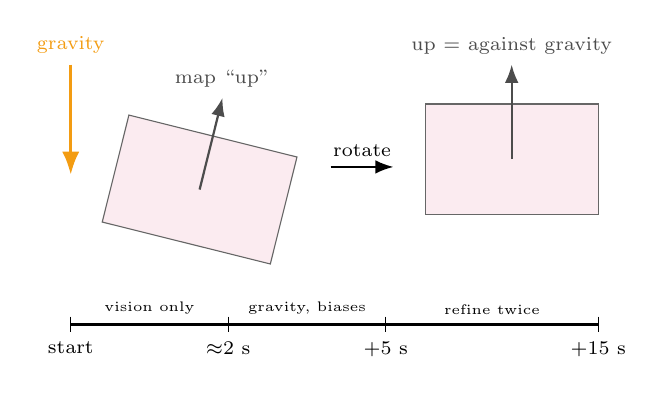
\begin{tikzpicture}[font=\scriptsize]
    \begin{scope}[rotate=-14]
      \draw[black!60, fill=orbc!10] (0,0) rectangle (2.2,1.4);
      \draw[-{Latex}, thick, black!70] (1.1,0.7) -- (1.1,1.9) node[above]{map ``up''};
    \end{scope}
    \draw[-{Latex}, very thick, dimu] (-0.4,2.0) -- (-0.4,0.6) node[pos=0, above]{gravity};
    \draw[-{Latex}, thick] (2.9,0.7) -- (3.7,0.7) node[midway, above]{rotate};
    \draw[black!60, fill=orbc!10] (4.1,0.1) rectangle (6.3,1.5);
    \draw[-{Latex}, thick, black!70] (5.2,0.8) -- (5.2,2.0) node[above]{up $=$ against gravity};
    \draw[thick] (-0.4,-1.3) -- (6.3,-1.3);
    \foreach \x/\l in {-0.4/start, 1.6/$\approx$2 s, 3.6/+5 s, 6.3/+15 s}
      {\draw (\x,-1.2) -- (\x,-1.4); \node[below] at (\x,-1.4) {\l};}
    \node[above, font=\tiny] at (0.6,-1.3) {vision only};
    \node[above, font=\tiny] at (2.6,-1.3) {gravity, biases};
    \node[above, font=\tiny] at (4.95,-1.3) {refine twice};
  \end{tikzpicture}}%
  {Watch $\approx$2 s of vision only (10 keyframes), solve for gravity, biases
   and speed, then rotate the whole map so ``up'' matches gravity.}
  {Before the IMU can help, the system must know which way is down and the
   IMU's biases. Those can only be seen once the robot moves.}
  {first $\approx$10 keyframes + IMU steps}
  {gravity-aligned map, biases, velocity}
  {Gravity is observed only while the robot turns. The published pose changes frame at this instant.}
  {\repo{performance.csv}: imu\_initialized, inertial\_ba1/2;
   \repo{local_mapping.csv}: initialisation time}
  \src{Ours (fork patch 15): initialise even with a keyframe backlog; do not reset the map when the robot stands still at the start.}
\end{frame}

% ---------------------------------------------------------------- ORB-7
\begin{frame}{1.2.7 \;ORB-7 \;Place recognition: have I been here before?}
  \hl{ORB7}\res{\R{2}{}}
  \compbody{\orbstrip}{orbc}{%
  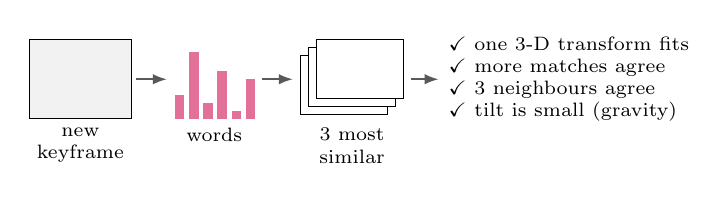
\begin{tikzpicture}[font=\scriptsize]
    \draw[fill=black!5] (0,0) rectangle (1.3,1.0); \node[below, align=center] at (0.65,0) {new\\keyframe};
    \draw[arr] (1.35,0.5) -- (1.75,0.5);
    \foreach \i/\h in {0/0.3,1/0.85,2/0.2,3/0.6,4/0.1,5/0.5} \fill[orbc!70] (1.85+\i*0.18,0) rectangle ++(0.12,\h);
    \node[below] at (2.35,0) {words};
    \draw[arr] (2.95,0.5) -- (3.35,0.5);
    \foreach \k in {0,1,2} \draw[fill=white] (3.45+\k*0.1,0.05+\k*0.1) rectangle ++(1.1,0.75);
    \node[below, align=center] at (4.1,0) {3 most\\similar};
    \draw[arr] (4.85,0.5) -- (5.2,0.5);
    \node[anchor=west, align=left] at (5.2,0.5)
      {$\checkmark$ one 3-D transform fits\\$\checkmark$ more matches agree\\
       $\checkmark$ 3 neighbours agree\\$\checkmark$ tilt is small (gravity)};
  \end{tikzpicture}}%
  {A fast search by visual words finds candidates; four geometric checks decide.
   Pass all four and a revisit is accepted.}
  {Tracking only knows the last few seconds, so drift builds up. Recognising an
   old place, however far you have drifted, is what removes it.}
  {each new keyframe}
  {a confirmed revisit + the transform --- or nothing}
  {Two identical-looking places can pass every check. A real revisit can be missed.}
  {\repo{loop_closing.csv}: one row per detection event}
\end{frame}

% ---------------------------------------------------------------- ORB-8
\begin{frame}{1.2.8 \;ORB-8 \;Loop correction, map merging and the Atlas}
  \hl{ORB8}\res{\R{2}{}, \R{3}{}}
  \compbody{\orbstrip}{orbc}{%
  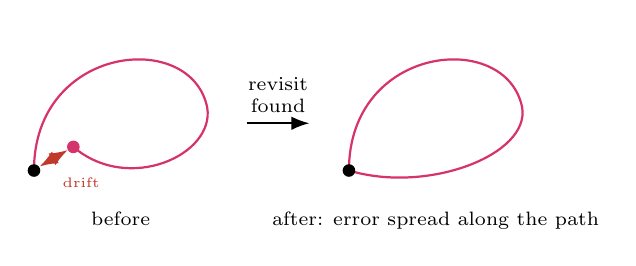
\begin{tikzpicture}[font=\scriptsize]
    \draw[thick, orbc] (0,0) .. controls (0,1.6) and (2,1.8) .. (2.2,0.8)
                             .. controls (2.3,0.2) and (1.2,-0.3) .. (0.5,0.3);
    \node[pt=black] at (0,0) {}; \node[pt=orbc] at (0.5,0.3) {};
    \draw[hlc, thick, {Latex}-{Latex}] (0.07,0.05) -- (0.43,0.26);
    \node[text=hlc, font=\tiny] at (0.6,-0.15) {drift};
    \node[below] at (1.1,-0.4) {before};
    \draw[-{Latex}, thick] (2.7,0.6) -- (3.5,0.6) node[midway, above, align=center]{revisit\\found};
    \draw[thick, orbc] (4.0,0) .. controls (4.0,1.6) and (6.0,1.8) .. (6.2,0.8)
                            .. controls (6.3,0.2) and (5.0,-0.3) .. (4.0,0);
    \node[pt=black] at (4.0,0) {};
    \node[below] at (5.1,-0.4) {after: error spread along the path};
  \end{tikzpicture}}%
  {The error found at the revisit is spread back over the whole path (pose
   graph, then a full bundle adjustment). The same idea merges two maps.}
  {Fixing only the current pose would leave the rest of the map bent.}
  {a confirmed revisit (ORB-7)}
  {corrected map and path --- the pose can jump}
  {A false revisit applies a large wrong correction to the whole map.}
  {\repo{loop_closing.csv}: correction size in m and deg; jumps in \repo{vio.csv}}
  \src{Atlas: lost for more than 5 s $\rightarrow$ start a new map, merge it when a place is recognised.
       Ours: one switch, \texttt{loopClosing}, turns ORB-7 and ORB-8 (and merging) on or off together.}
\end{frame}

% ---------------------------------------------------------------- config
\begin{frame}{1.2.9 \;ORB-SLAM3 configuration}
  \centering
  \adjustbox{max width=\textwidth, max height=0.80\textheight}{%
  \begin{tabular}{l l l l l}
    \toprule
    & Parameter & Sim & Real rig & What it means \\
    \midrule
    ORB-1 & \texttt{Camera.type} & PinHole & KannalaBrandt8 & lens model: how a pixel maps to a direction \\
          & image size, \texttt{Camera.fps} & 1280$\times$720, 30 & 1920$\times$1080, 30 & what the node receives \\
          & \texttt{ORBextractor.nFeatures} & 1500 & 2000 & points kept per image \\
          & \texttt{scaleFactor} / \texttt{nLevels} & 1.2 / 8 & 1.2 / 8 & look at 8 image sizes, each 1.2$\times$ smaller \\
          & \texttt{iniThFAST} / \texttt{minThFAST} & 20 / 7 & 20 / 7 & corner strength; relaxed in dull areas \\
          & \texttt{Stereo.ThDepth} & 90 & 90 & ``close'' point = nearer than 90 $\times$ baseline \\
          & \textcolor{ourc}{\texttt{ORBextractor.useGPU}} & 1 & 0 & GPU extractor (our patch 10) \\
    \addlinespace
    ORB-2 & \texttt{IMU.Frequency} & 200 & 200 & IMU rate, Hz \\
          & \texttt{IMU.NoiseGyro} / \texttt{NoiseAcc} & 0.002 / 0.02 & 0.1 / 1.0 & how much each reading is trusted \\
          & \texttt{IMU.GyroWalk} / \texttt{AccWalk} & 1e-4 / 1e-3 & 1e-4 / 1e-3 & how fast the biases may drift \\
    \addlinespace
    ORB-6 & \textcolor{ourc}{\texttt{LocalMapping.initWithBacklog}} & 1 & 1 & initialise even with keyframes queued (patch 15) \\
          & \textcolor{ourc}{\texttt{LocalMapping.resetOnLowMotion}} & 0 & 0 & do not reset when standing still (patch 15) \\
    \addlinespace
    ORB-7/8 & \textcolor{ourc}{\texttt{loopClosing}} & 0 & 0 & base-file value; the on/off switch for revisits and merging \\
    \bottomrule
  \end{tabular}}
  \par\vspace{0.5em}
  \scriptsize\color{black!65}
  \textcolor{ourc}{\textbf{Amber}} = a key added by our fork.
  The real rig's IMU noise values were raised tenfold during commissioning.
  \src{\repo{orbslam3_ros2/config/wil_sim/stereo_imu.yaml}, \repo{orbslam3_ros2/config/wil/stereo_imu.yaml}}
\end{frame}

% =============================================================================
% 1.3  VINS-FUSION
% Sources: Qin, Li & Shen, VINS-Mono, IEEE T-RO 2018 (Fig. 2, sections IV-VIII);
% Qin & Shen, Online Temporal Calibration, IROS 2018; and
% vins_fusion_ros2/config/wil_sim/stereo_imu.yaml, config/wil/stereo_imu.yaml,
% vins/include/vins/estimator/parameters.h (WINDOW_SIZE = 10).
% =============================================================================
\section{1.3 VINS-Fusion}

\begin{frame}{1.3 \;VINS-Fusion: a sliding window over the last 10 keyframes}
  \centering
  \adjustbox{max width=\textwidth, max height=0.70\textheight}{%
  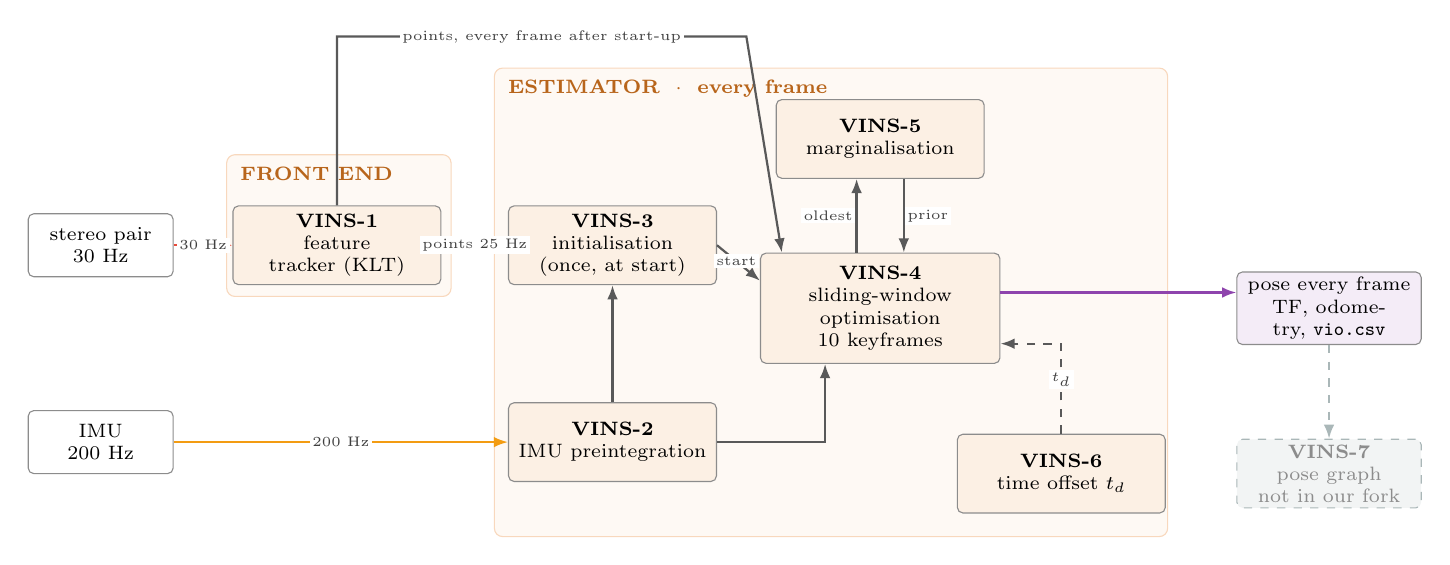
\begin{tikzpicture}[font=\scriptsize,
      cb/.style={box, fill=vinsc!12, text width=25mm, minimum height=10mm},
      bl/.style={font=\scriptsize\bfseries, text=vinsc!80!black, anchor=north west}]
    \fill[vinsc!5, draw=vinsc!30, rounded corners=3pt] (1.6,-0.05) rectangle (4.45,1.75);
    \node[bl] at (1.65,1.72) {FRONT END};
    \fill[vinsc!5, draw=vinsc!30, rounded corners=3pt] (5.0,-3.1) rectangle (13.55,2.85);
    \node[bl] at (5.05,2.82) {ESTIMATOR \;$\cdot$\; every frame};
    \node[box, text width=17mm] (st) at (0,0.6)  {stereo pair\\30 Hz};
    \node[box, text width=17mm] (im) at (0,-1.9) {IMU\\200 Hz};
    \node[cb, VINS1] (v1) at (3.0,0.6)  {\textbf{VINS-1}\\feature tracker (KLT)};
    \node[cb, VINS3] (v3) at (6.5,0.6)  {\textbf{VINS-3}\\initialisation\\(once, at start)};
    \node[cb, VINS2] (v2) at (6.5,-1.9) {\textbf{VINS-2}\\IMU preintegration};
    \node[cb, VINS4, text width=29mm, minimum height=14mm] (v4) at (9.9,-0.2)
      {\textbf{VINS-4}\\sliding-window optimisation\\10 keyframes};
    \node[cb, VINS5] (v5) at (9.9,1.95) {\textbf{VINS-5}\\marginalisation};
    \node[cb, VINS6] (v6) at (12.2,-2.3) {\textbf{VINS-6}\\time offset $t_d$};
    \node[box, text width=22mm, fill=dpose!10] (out) at (15.6,-0.2)
      {pose every frame\\TF, odometry, \repo{vio.csv}};
    \node[box, off, text width=22mm, VINS7] (v7) at (15.6,-2.3) {\textbf{VINS-7}\\pose graph\\not in our fork};
    \draw[arr, dimg] (st) -- node[rate]{30 Hz} (v1);
    \draw[arr, dimu] (im) -- node[rate]{200 Hz} (v2);
    \draw[arr] (v1) -- node[rate]{points 25 Hz} (v3);
    \draw[arr] (v2) -- (v3);
    \draw[arr] (v3.east) -- node[rate, pos=0.45]{start} ($(v4.west)+(0,0.35)$);
    \draw[arr] (v2.east) -| ($(v4.south)+(-0.7,0)$);
    \draw[arr] (v1.north) |- (8.2,3.25) -- ($(v4.north)+(-1.25,0)$);
    \node[rate] at (5.6,3.25) {points, every frame after start-up};
    \draw[arr] ($(v4.north)+(-0.3,0)$) -- node[rate, left]{oldest} ($(v5.south)+(-0.3,0)$);
    \draw[arr] ($(v5.south)+(0.3,0)$) -- node[rate, right]{prior} ($(v4.north)+(0.3,0)$);
    \draw[darr] (v6.north) |- node[rate, pos=0.3]{$t_d$} ($(v4.east)+(0,-0.45)$);
    \draw[arr, dpose] ($(v4.east)+(0,0.2)$) -- ($(out.west)+(0,0.2)$);
    \draw[darr, offc] (out) -- (v7);
  \end{tikzpicture}}
  \par\vspace{0.3em}
  \small The front end follows points from frame to frame; the estimator fits
  the last 10 keyframes to every camera and IMU measurement at once. Unlike
  ORB-SLAM3 there is \textbf{no map to come back to}: what leaves the window
  is summarised, never revisited.
  \src{After Qin, Li \& Shen, VINS-Mono, IEEE T-RO 2018, Fig.~2.}
\end{frame}

% ---------------------------------------------------------------- VINS-1
\begin{frame}{1.3.1 \;VINS-1 \;Feature tracker: follow the same points from frame to frame}
  \hl{VINS1}\res{\R{5}{}, \R{6}{}, \R{7}{}, \R{8}{}}
  \compbody{\vinsstrip}{vinsc}{%
  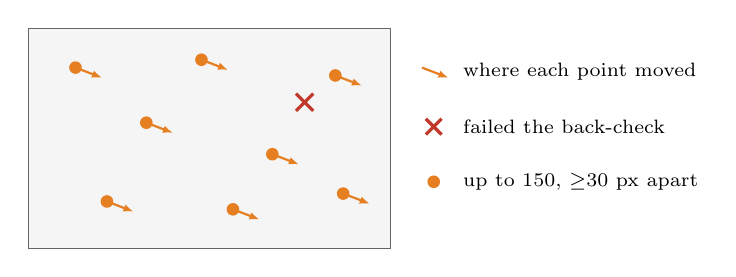
\begin{tikzpicture}[font=\scriptsize]
    \draw[black!60, fill=black!4] (0,0) rectangle (4.6,2.8);
    \foreach \x/\y in {0.6/2.3,1.5/1.6,2.2/2.4,3.1/1.2,3.9/2.2,1.0/0.6,2.6/0.5,4.0/0.7} {
      \node[pt=vinsc] at (\x,\y) {};
      \draw[-{Latex[length=1.3mm]}, vinsc, thick] (\x,\y) -- ++(0.34,-0.13);}
    \draw[bad, very thick] (3.4,1.75) -- ++(0.22,0.22) (3.4,1.97) -- ++(0.22,-0.22);
    \draw[-{Latex[length=1.3mm]}, vinsc, thick] (5.0,2.3) -- ++(0.34,-0.13);
    \node[anchor=west] at (5.4,2.25) {where each point moved};
    \draw[bad, very thick] (5.05,1.45) -- ++(0.2,0.2) (5.05,1.65) -- ++(0.2,-0.2);
    \node[anchor=west] at (5.4,1.55) {failed the back-check};
    \node[pt=vinsc] at (5.15,0.85) {};
    \node[anchor=west] at (5.4,0.85) {up to 150, $\ge$30 px apart};
  \end{tikzpicture}}%
  {Follow each point forward into the new image, then backward to check; drop
   those that do not come back. Top up with new corners.}
  {To measure motion you need the same points in consecutive images. Following
   each by its local patch (optical flow) is cheaper than re-describing it.}
  {stereo pair, 30 Hz}
  {tracked points (ID + position), 25 Hz sim / 20 Hz real}
  {Blank walls leave little to follow. Points near a fisheye's edge are badly modelled.}
  {\repo{frontend.csv}: feature\_count, stereo\_feature\_count, tracking time}
  \src{Ours: a mask (\texttt{setMask}) can forbid image regions --- used for the real fisheye's outer ring (\texttt{fov\_mask\_deg}) and for YOLO.}
\end{frame}

% ---------------------------------------------------------------- VINS-1 inside
% Where the points come from. Read from vins/src/featureTracker/feature_tracker.cpp:
% KLT calcOpticalFlowPyrLK 21x21, 3 levels (L154-178); reverse check <= 0.5 px
% (L183-193); setMask with min_feature_distance circles, seeded from the dynamic
% mask (L53); goodFeaturesToTrack(max - current, 0.01, min_dist, mask) (L307);
% rejectWithF() commented out (L297); first frame skips tracking (L154).
\begin{frame}{1.3.1 \;VINS-1 \;Inside: where the points come from}
  \hl{VINS1}\res{\R{5}{}, \R{6}{}, \R{7}{}, \R{8}{}}
  \vinsstrip\par\vspace{0.3em}
  \centering
  \adjustbox{max width=\textwidth, max height=0.60\textheight}{%
  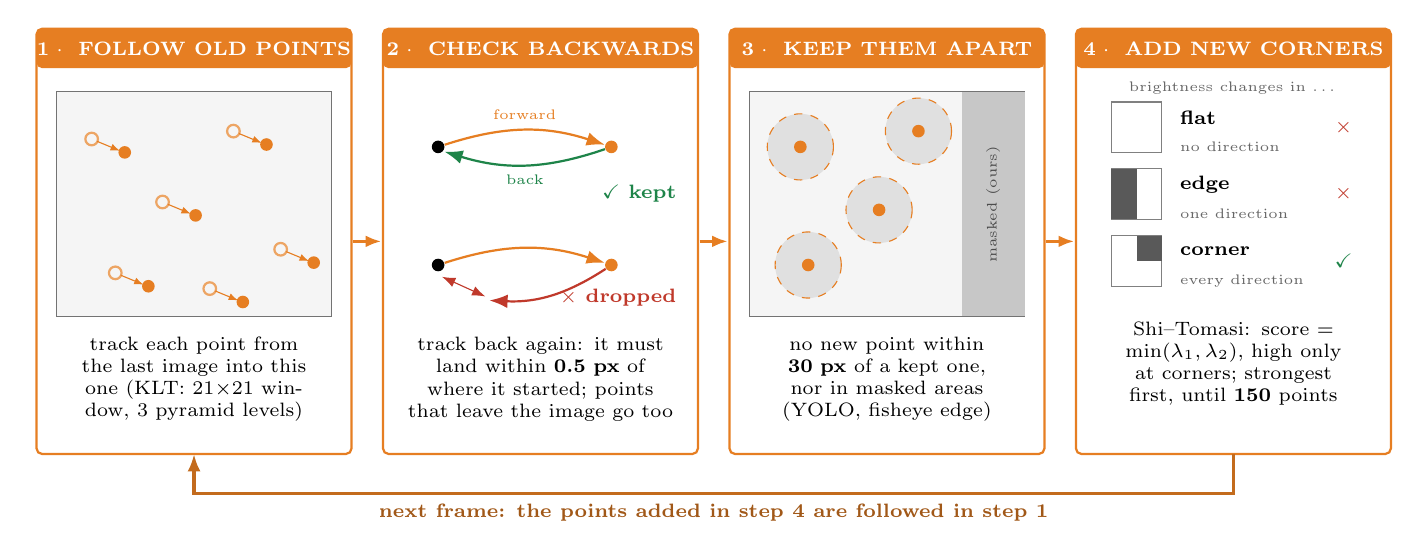
\begin{tikzpicture}[font=\scriptsize,
      capt/.style={align=center, text width=35mm, font=\scriptsize}]
    \foreach \i/\x/\t in {1/0/FOLLOW OLD POINTS, 2/4.4/CHECK BACKWARDS, 3/8.8/KEEP THEM APART, 4/13.2/ADD NEW CORNERS} {
      \draw[vinsc, line width=0.8pt, rounded corners=2pt, fill=white] (\x,0) rectangle ++(4.0,5.4);
      \fill[vinsc, rounded corners=2pt] (\x,4.9) rectangle ++(4.0,0.5);
      \node[text=white, font=\scriptsize\bfseries] at (\x+2.0,5.15) {\i \;$\cdot$\; \t};}
    \foreach \x in {4.0,8.4,12.8} \draw[-{Latex[length=2mm]}, very thick, vinsc] (\x+0.02,2.7) -- (\x+0.38,2.7);
    % ---- 1: KLT, previous position (hollow) -> current position (filled)
    \draw[black!55, fill=black!4] (0.25,1.75) rectangle (3.75,4.6);
    \foreach \x/\y in {0.7/4.0, 1.6/3.2, 2.5/4.1, 3.1/2.6, 1.0/2.3, 2.2/2.1} {
      \draw[vinsc!70, thick] (\x,\y) circle (0.08);
      \draw[-{Latex[length=1.2mm]}, vinsc] (\x+0.07,\y-0.03) -- (\x+0.36,\y-0.15);
      \node[pt=vinsc] at (\x+0.42,\y-0.17) {};}
    \node[capt] at (2.0,0.95) {track each point from the last image into this one (KLT: 21$\times$21 window, 3 pyramid levels)};
    % ---- 2: reverse check
    \begin{scope}[shift={(4.4,0)}]
      \node[pt=black] (a) at (0.7,3.9) {}; \node[pt=vinsc] (a2) at (2.9,3.9) {};
      \draw[-{Latex}, thick, vinsc] (a) to[bend left=18] node[above, font=\tiny]{forward} (a2);
      \draw[-{Latex}, thick, good] (a2) to[bend left=18] node[below, font=\tiny]{back} ($(a)+(0.08,-0.06)$);
      \node[text=good, font=\scriptsize\bfseries, anchor=east] at (3.85,3.3) {$\checkmark$ kept};
      \node[pt=black] (b) at (0.7,2.4) {}; \node[pt=vinsc] (b2) at (2.9,2.4) {};
      \draw[-{Latex}, thick, vinsc] (b) to[bend left=18] (b2);
      \draw[-{Latex}, thick, bad] (b2) to[bend left=18] (1.35,1.95);
      \draw[{Latex}-{Latex}, bad] (0.75,2.25) -- (1.3,2.0);
      \node[text=bad, font=\scriptsize\bfseries, anchor=east] at (3.85,1.98) {$\times$ dropped};
    \end{scope}
    \node[capt] at (6.4,0.95) {track back again: it must land within \textbf{0.5 px} of where it started; points that leave the image go too};
    % ---- 3: mask
    \begin{scope}[shift={(8.8,0)}]
      \draw[black!55, fill=black!4] (0.25,1.75) rectangle (3.75,4.6);
      \fill[black!22] (2.95,1.75) rectangle (3.75,4.6);
      \node[rotate=90, font=\tiny, text=black!70] at (3.35,3.17) {masked (ours)};
      \foreach \x/\y in {0.9/3.9, 1.9/3.1, 1.0/2.4, 2.4/4.1} {
        \fill[black!12] (\x,\y) circle (0.42);
        \draw[vinsc, dashed] (\x,\y) circle (0.42);
        \node[pt=vinsc] at (\x,\y) {};}
    \end{scope}
    \node[capt] at (10.8,0.95) {no new point within \textbf{30 px} of a kept one, nor in masked areas (YOLO, fisheye edge)};
    % ---- 4: Shi-Tomasi top-up
    \begin{scope}[shift={(13.2,0)}]
      \foreach \c/\lab/\ok/\yy in {0/flat/0/4.15, 1/edge/0/3.3, 2/corner/1/2.45} {
        \draw[black!50] (0.45,\yy-0.32) rectangle ++(0.64,0.64);
        \ifnum\c=1 \fill[black!65] (0.45,\yy-0.32) rectangle ++(0.32,0.64); \fi
        \ifnum\c=2 \fill[black!65] (0.77,\yy) rectangle ++(0.32,0.32); \fi
        \node[anchor=west, font=\scriptsize] at (1.2,\yy+0.12) {\textbf{\lab}};
        \ifnum\ok=1 \node[text=good, font=\scriptsize\bfseries] at (3.4,\yy) {$\checkmark$};
        \else       \node[text=bad, font=\scriptsize\bfseries] at (3.4,\yy) {$\times$}; \fi}
      \node[font=\tiny, text=black!60] at (2.0,4.65) {brightness changes in \ldots};
      \node[font=\tiny, text=black!60, anchor=west] at (1.2,3.9) {no direction};
      \node[font=\tiny, text=black!60, anchor=west] at (1.2,3.05) {one direction};
      \node[font=\tiny, text=black!60, anchor=west] at (1.2,2.2) {every direction};
    \end{scope}
    \node[capt] at (15.2,1.15) {Shi--Tomasi: score = $\min(\lambda_1,\lambda_2)$, high only at corners; strongest first, until \textbf{150} points};
    \draw[-{Latex[length=2.2mm]}, very thick, vinsc!85!black] (15.2,0) -- (15.2,-0.5) --
      node[below, font=\scriptsize\bfseries, text=vinsc!70!black]{next frame: the points added in step 4 are followed in step 1}
      (2.0,-0.5) -- (2.0,0);
  \end{tikzpicture}}
  \par\vspace{0.15em}
  \scriptsize\color{black!70}
  \textbf{Frame 0:} step 4 only --- nothing to follow yet, so all 150 points are new.
  \textbf{Frame 1 onward:} 1$\rightarrow$2$\rightarrow$3$\rightarrow$4, every frame.
  Each point is also tracked left$\rightarrow$right for depth and turned into a ray.
  \src{\repo{feature_tracker.cpp}: \texttt{rejectWithF} (the fundamental-matrix test) is commented out in our fork, so \texttt{F\_threshold} has no effect.}
\end{frame}

% ---------------------------------------------------------------- VINS-2
\begin{frame}{1.3.2 \;VINS-2 \;IMU preintegration: the same idea as ORB-2}
  \hl{VINS2}\res{\R{8}{}}
  \compbody{\vinsstrip}{vinsc}{%
  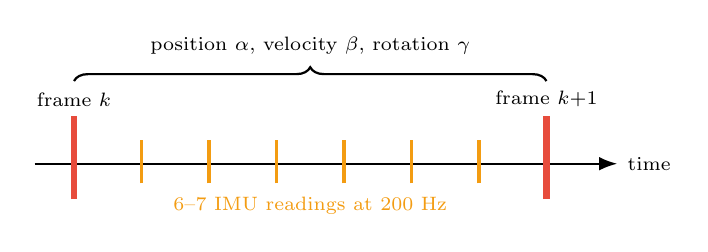
\begin{tikzpicture}[font=\scriptsize]
    \draw[thick,-{Latex}] (0,0) -- (7.4,0) node[right]{time};
    \foreach \x/\l in {0.5/frame $k$, 6.5/frame $k{+}1$} {
      \draw[line width=2.4pt, dimg] (\x,-0.45) -- (\x,0.6);
      \node[above] at (\x,0.6) {\l};}
    \foreach \k in {1,...,6} \draw[dimu, line width=1.2pt]
      ({0.5+\k*6/7},-0.25) -- ({0.5+\k*6/7},0.3);
    \node[below, text=dimu] at (3.5,-0.3) {6--7 IMU readings at 200 Hz};
    \draw[decorate, decoration={brace, amplitude=5pt}, thick]
      (0.5,1.05) -- node[above=6pt]{position $\alpha$, velocity $\beta$, rotation $\gamma$} (6.5,1.05);
  \end{tikzpicture}}%
  {If the bias estimate changes a little, the summary is corrected by a formula
   instead of being added up again.}
  {Same job as ORB-2: summarise the IMU readings between two frames, once.}
  {IMU, 200 Hz}
  {one motion step + uncertainty per frame pair}
  {Wrong noise values; IMU gaps; a wrong gravity magnitude (\texttt{g\_norm}).}
  {\repo{backend.csv}: imu\_wait\_ms, imu\_propagation\_ms}
  \src{In simulation VINS-Fusion and ORB-SLAM3 are given identical IMU noise values.}
\end{frame}

% ---------------------------------------------------------------- VINS-3
\begin{frame}{1.3.3 \;VINS-3 \;Initialisation: start the estimator from nothing}
  \hl{VINS3}
  \compbody{\vinsstrip}{vinsc}{%
  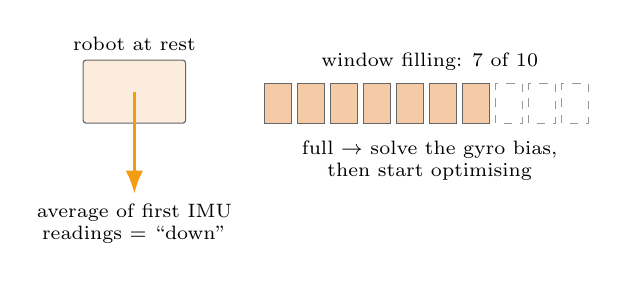
\begin{tikzpicture}[font=\scriptsize]
    \draw[black!60, fill=vinsc!15, rounded corners=1pt] (0,0) rectangle (1.3,0.8);
    \node[above] at (0.65,0.8) {robot at rest};
    \draw[-{Latex}, very thick, dimu] (0.65,0.4) -- (0.65,-0.9);
    \node[below, align=center] at (0.65,-0.9) {average of first IMU\\readings $=$ ``down''};
    \foreach \k in {0,...,6} \draw[black!60, fill=vinsc!40] (2.3+\k*0.42,0) rectangle ++(0.34,0.5);
    \foreach \k in {7,8,9} \draw[black!40, dashed] (2.3+\k*0.42,0) rectangle ++(0.34,0.5);
    \node[above] at (4.4,0.55) {window filling: 7 of 10};
    \node[below, align=center] at (4.4,-0.1) {full $\rightarrow$ solve the gyro bias,\\then start optimising};
  \end{tikzpicture}}%
  {Stereo makes this simpler than the paper's single camera: depth is known,
   the first IMU readings give ``down'', the gyro bias is solved once the window is full.}
  {The optimiser needs a sensible first guess of speed, gravity and biases, or
   it settles on a wrong answer.}
  {first window of frames + IMU}
  {starting states for the sliding window}
  {Moving too early; a wrong \texttt{g\_norm} tilts the starting gravity.}
  {\repo{backend.csv}: solver\_state, initialized\_this\_frame; \repo{events.csv}}
\end{frame}

% ---------------------------------------------------------------- VINS-4
\begin{frame}{1.3.4 \;VINS-4 \;Sliding window: fit the last 10 keyframes to everything measured}
  \hl{VINS4}\res{\R{5}{}, \R{6}{}, \R{7}{}}
  \compbody{\vinsstrip}{vinsc}{%
  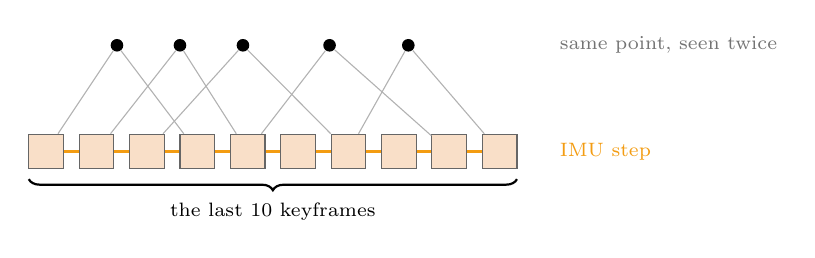
\begin{tikzpicture}[font=\scriptsize]
    \foreach \k in {0,...,9} \node[draw=black!60, fill=vinsc!25, minimum size=4.4mm, inner sep=0pt] (w\k) at (\k*0.64,0) {};
    \foreach \k [evaluate=\k as \n using int(\k+1)] in {0,...,8} \draw[dimu, very thick] (w\k) -- (w\n);
    \foreach \x/\a/\b in {0.9/0/3, 1.7/1/4, 2.5/2/6, 3.6/4/8, 4.6/6/9} {
      \node[pt=black] (f) at (\x,1.35) {};
      \draw[black!30] (f) -- (w\a); \draw[black!30] (f) -- (w\b);}
    \draw[decorate, decoration={brace, amplitude=4pt, mirror}, thick]
      (-0.22,-0.35) -- node[below=5pt]{the last 10 keyframes} (5.98,-0.35);
    \node[anchor=west, text=dimu] at (6.4,0.0) {IMU step};
    \node[anchor=west, text=black!55] at (6.4,1.35) {same point, seen twice};
  \end{tikzpicture}}%
  {Every frame: adjust all 10 keyframes (position, speed, rotation, biases) and
   every point's depth until the IMU steps and the camera views agree.}
  {Using every measurement ever made would get slower forever. A fixed window
   keeps the cost constant, so it stays real-time.}
  {points (VINS-1) + IMU steps (VINS-2)}
  {pose, velocity, biases every frame $\rightarrow$ TF, odometry, \repo{vio.csv}}
  {The solve runs past its 0.08\,s budget; bad points pull the answer.}
  {\repo{backend.csv}: visual\_update\_ms; \repo{estimator_state.csv}: pose, velocity, biases}
\end{frame}

% ---------------------------------------------------------------- VINS-5
\begin{frame}{1.3.5 \;VINS-5 \;Marginalisation: let the window slide without forgetting}
  \hl{VINS5}
  \compbody{\vinsstrip}{vinsc}{%
  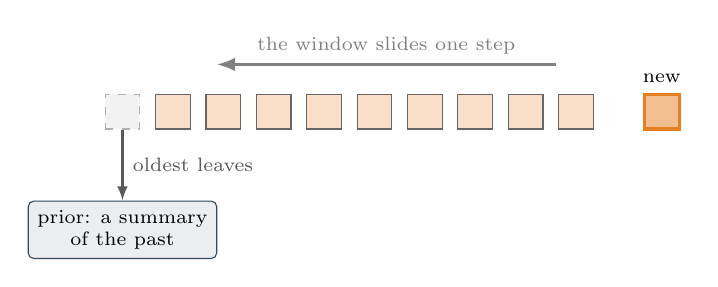
\begin{tikzpicture}[font=\scriptsize]
    \node[draw=black!30, dashed, fill=black!5, minimum size=4.4mm, inner sep=0pt] (w0) at (0,0) {};
    \foreach \k in {1,...,9} \node[draw=black!60, fill=vinsc!25, minimum size=4.4mm, inner sep=0pt] (w\k) at (\k*0.64,0) {};
    \node[draw=vinsc, very thick, fill=vinsc!50, minimum size=4.4mm, inner sep=0pt] (wn) at (6.85,0) {};
    \node[above] at (wn.north) {new};
    \node[draw=mapcol, fill=mapcol!10, rounded corners=2pt, align=center] (pr) at (0,-1.5) {prior: a summary\\of the past};
    \draw[arr] (w0) -- node[right]{oldest leaves} (pr);
    \draw[-{Latex}, thick, black!50] (5.5,0.6) -- node[above]{the window slides one step} (1.2,0.6);
  \end{tikzpicture}}%
  {The oldest keyframe is folded into a prior. If the newest frame is not a
   keyframe (parallax under 10 px), its images are dropped and its IMU step kept.}
  {When a keyframe enters, the oldest must leave. Deleting it outright would
   throw away what it told us.}
  {the window after each solve}
  {a prior for the next solve}
  {The past is frozen into the prior: drift builds up smoothly and is never undone here.}
  {\repo{backend.csv}: marginalization, keyframe}
\end{frame}

% ---------------------------------------------------------------- VINS-6
\begin{frame}{1.3.6 \;VINS-6 \;Time offset: are the camera and IMU clocks aligned?}
  \hl{VINS6}
  \compbody{\vinsstrip}{vinsc}{%
  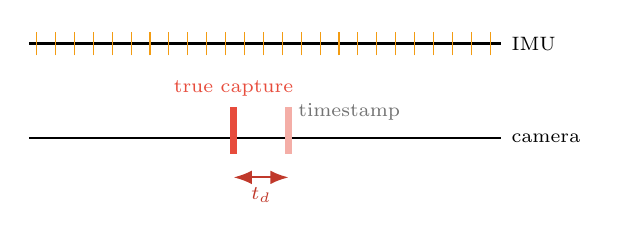
\begin{tikzpicture}[font=\scriptsize]
    \draw[thick] (0,1.2) -- (6,1.2) node[right]{IMU};
    \foreach \k in {0,...,24} \draw[dimu] ({0.1+\k*0.24},1.05) -- ++(0,0.3);
    \draw[thick] (0,0) -- (6,0) node[right]{camera};
    \draw[dimg, line width=2.4pt] (2.6,-0.2) -- (2.6,0.4);
    \node[above, text=dimg] at (2.6,0.4) {true capture};
    \draw[dimg!45, line width=2.4pt] (3.3,-0.2) -- (3.3,0.4);
    \node[above right, text=black!55] at (3.3,0.1) {timestamp};
    \draw[{Latex}-{Latex}, hlc, thick] (2.6,-0.5) -- node[below]{$t_d$} (3.3,-0.5);
  \end{tikzpicture}}%
  {If the timestamp is late by $t_d$, each image is paired with the wrong IMU
   motion. VINS can estimate $t_d$; ours fixes it at 0.}
  {The calibration paper shows VINS tolerates only about 6\,ms of clock
   mismatch before accuracy suffers.}
  {feature velocities, the window}
  {$t_d$ --- fixed at 0 in both our configs}
  {On the real rig an unmodelled offset would look like a motion error.}
  {\repo{estimator_state.csv}: time\_delay\_s; config \texttt{estimate\_td}}
  \src{Qin \& Shen, Online Temporal Calibration for Monocular Visual-Inertial Systems, IROS 2018. The simulator's clock is exact by construction.}
\end{frame}

% ---------------------------------------------------------------- VINS-7
\begin{frame}{1.3.7 \;VINS-7 \;Loop closure and pose graph: in VINS, but not in our fork}
  \hl{VINS7}
  \compbody{\vinsstrip}{offc!80!black}{%
  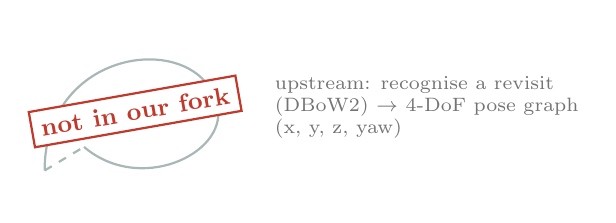
\begin{tikzpicture}[font=\scriptsize]
    \draw[thick, offc] (0,0) .. controls (0,1.6) and (2,1.8) .. (2.2,0.8)
                            .. controls (2.3,0.2) and (1.2,-0.3) .. (0.5,0.3);
    \draw[offc, dashed, thick] (0,0) -- (0.5,0.3);
    \node[draw=bad, thick, rotate=10, text=bad, font=\small\bfseries, fill=white] at (1.15,0.75) {not in our fork};
    \node[anchor=west, align=left, text=black!55] at (2.8,0.8)
      {upstream: recognise a revisit\\(DBoW2) $\rightarrow$ 4-DoF pose graph\\(x, y, z, yaw)};
  \end{tikzpicture}}%
  {Roll and pitch are already fixed by gravity, so upstream VINS optimises only
   x, y, z and heading when it closes a loop.}
  {Without it, VINS-Fusion never recognises a revisited place: it is pure odometry.}
  {--- (not run)}
  {---}
  {Drift inside VINS is never removed; in this system only RTAB-Map uses revisits.}
  {none: the module does not run}
\end{frame}

% ---------------------------------------------------------------- config
\begin{frame}{1.3.8 \;VINS-Fusion configuration}
  \centering
  \adjustbox{max width=\textwidth, max height=0.80\textheight}{%
  \begin{tabular}{l l l l l}
    \toprule
    & Parameter & Sim & Real rig & What it means \\
    \midrule
    VINS-1 & camera model, image size & pinhole, 1280$\times$720 & Kannala-Brandt, 1920$\times$1080 & lens model, what the node receives \\
           & \texttt{max\_cnt} / \texttt{min\_dist} & 150 / 30 px & 150 / 30 px & points tracked, minimum spacing \\
           & \texttt{freq} & 25 Hz & 20 Hz & tracker output rate \\
           & \texttt{flow\_back} / \texttt{F\_threshold} & on / \textcolor{bad}{unused} & on / \textcolor{bad}{unused} & back-check 0.5 px; F-test commented out in our fork \\
           & \textcolor{ourc}{\texttt{fov\_mask\_deg}} & --- & 70$^\circ$ & ignore the fisheye's outer ring \\
    \addlinespace
    VINS-2 & \texttt{acc\_n} / \texttt{gyr\_n} & 0.02 / 0.002 & 0.1 / 0.01 & how much each IMU reading is trusted \\
           & \texttt{acc\_w} / \texttt{gyr\_w} & 1e-3 / 1e-4 & 1e-3 / 1e-4 & how fast the biases may drift \\
           & \texttt{g\_norm} & 9.8 & 9.8858 & gravity magnitude (real: measured at rest) \\
    \addlinespace
    VINS-4 & \texttt{WINDOW\_SIZE} & 10 & 10 & keyframes in the window (compile-time) \\
           & \texttt{max\_solver\_time} / iterations & 0.08 s / 100 & 0.08 s / 100 & solver budget per frame \\
    VINS-5 & \texttt{keyframe\_parallax} & 10 px & 10 px & parallax that makes a keyframe \\
    \addlinespace
    VINS-6 & \texttt{estimate\_td} / \texttt{td} & 0 / 0.0 & 0 / --- & time offset fixed, not estimated \\
           & \texttt{estimate\_extrinsic} & 0 & 0 & camera--IMU mounting held fixed \\
    \bottomrule
  \end{tabular}}
  \par\vspace{0.5em}
  \scriptsize\color{black!65}\textcolor{ourc}{\textbf{Amber}} = a parameter added by our fork.
  \src{\repo{vins_fusion_ros2/config/wil_sim/stereo_imu.yaml}, \repo{vins_fusion_ros2/config/wil/stereo_imu.yaml}, \repo{parameters.h}}
\end{frame}

% =============================================================================
% 1.4  RTAB-MAP
% Sources: Labbe & Michaud, RTAB-Map, J. Field Robotics 2019 (Fig. 1, 3.3-3.6);
% vslam_navigation/launch/rtabmap.launch.py; the run's launch.log (rosparams);
% rtabmap 0.23 Parameters.h for library defaults; scripts/rtab_camera_shim.py
% and scripts/correction_gate.py for the two nodes this project added.
% =============================================================================
\section{1.4 RTAB-Map}

\begin{frame}{1.4 \;RTAB-Map: a memory of places, and the map Nav2 plans on}
  \centering
  \adjustbox{max width=\textwidth, max height=0.70\textheight}{%
  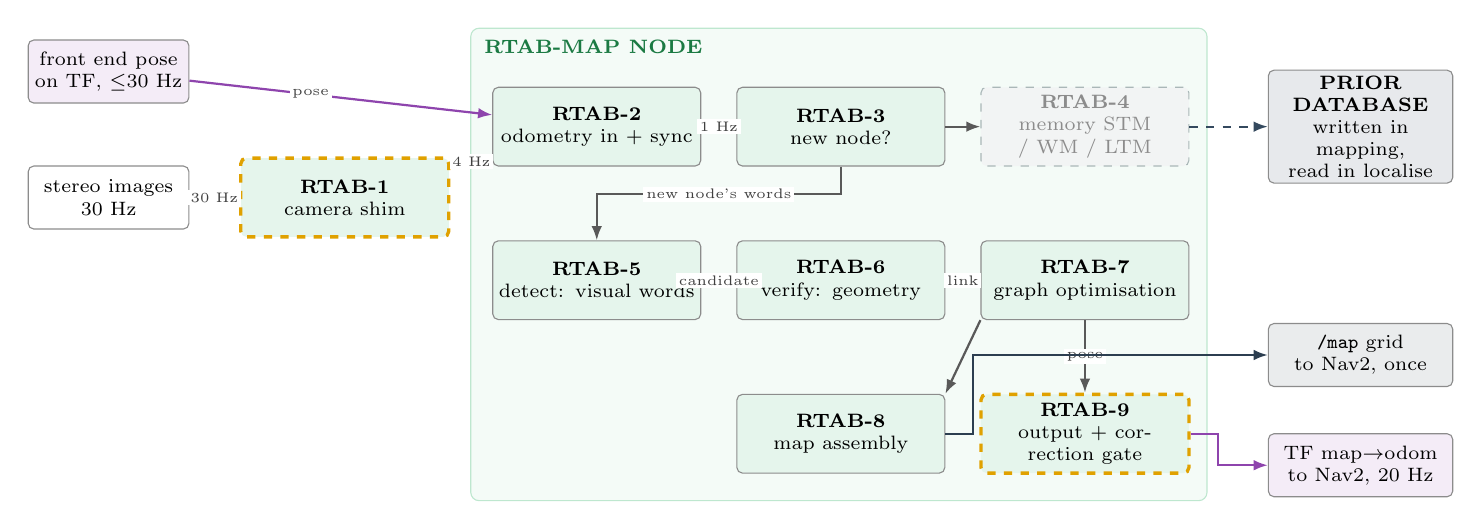
\begin{tikzpicture}[font=\scriptsize,
      cb/.style={box, fill=rtabc!12, text width=25mm, minimum height=10mm},
      bl/.style={font=\scriptsize\bfseries, text=rtabc!70!black, anchor=north west}]
    \fill[rtabc!5, draw=rtabc!30, rounded corners=3pt] (4.6,-4.45) rectangle (13.95,1.55);
    \node[bl] at (4.65,1.52) {RTAB-MAP NODE};
    \node[box, text width=19mm, fill=dpose!10] (fe) at (0,1.0) {front end pose\\on TF, $\le$30 Hz};
    \node[box, text width=19mm] (cams) at (0,-0.6) {stereo images\\30 Hz};
    \node[cb, ours, RTAB1] (r1) at (3.0,-0.6) {\textbf{RTAB-1}\\camera shim};
    \node[cb, RTAB2] (r2) at (6.2,0.3)  {\textbf{RTAB-2}\\odometry in + sync};
    \node[cb, RTAB3] (r3) at (9.3,0.3)  {\textbf{RTAB-3}\\new node?};
    \node[cb, off, RTAB4] (r4) at (12.4,0.3) {\textbf{RTAB-4}\\memory STM / WM / LTM};
    \node[cb, RTAB5] (r5) at (6.2,-1.65) {\textbf{RTAB-5}\\detect: visual words};
    \node[cb, RTAB6] (r6) at (9.3,-1.65) {\textbf{RTAB-6}\\verify: geometry};
    \node[cb, RTAB7] (r7) at (12.4,-1.65) {\textbf{RTAB-7}\\graph optimisation};
    \node[cb, RTAB8] (r8) at (9.3,-3.6) {\textbf{RTAB-8}\\map assembly};
    \node[cb, ours, RTAB9] (r9) at (12.4,-3.6) {\textbf{RTAB-9}\\output + correction gate};
    \node[box, text width=22mm, fill=mapcol!12] (db) at (15.9,0.3) {\textbf{PRIOR DATABASE}\\written in mapping,\\read in localise};
    \node[box, text width=22mm, fill=dmap!10] (om) at (15.9,-2.6) {\texttt{/map} grid\\to Nav2, once};
    \node[box, text width=22mm, fill=dpose!10] (ot) at (15.9,-4.0) {TF map$\rightarrow$odom\\to Nav2, 20 Hz};
    \draw[arr, dpose] (fe) -- node[rate, pos=0.4]{pose} (r2);
    \draw[arr, dimg] (cams) -- node[rate]{30 Hz} (r1);
    \draw[arr, dimg] (r1) -- node[rate]{4 Hz} (r2);
    \draw[arr] (r2) -- node[rate]{1 Hz} (r3);
    \draw[arr] (r3) -- (r4);
    \draw[arr] (r3.south) -- ++(0,-0.35) -| node[rate, pos=0.25]{new node's words} (r5.north);
    \draw[arr] (r5) -- node[rate]{candidate} (r6);
    \draw[arr] (r6) -- node[rate]{link} (r7);
    \draw[arr] (r7.south) -- node[rate]{pose} (r9.north);
    \draw[arr] (r7.south west) -- (r8.north east);
    \draw[darr, mapcol] (r4.east) -- (db.west);
    \draw[arr, dmap] (r8.east) -- ++(0.35,0) |- (om.west);
    \draw[arr, dpose] (r9.east) -- ++(0.35,0) |- (ot.west);
  \end{tikzpicture}}
  \par\vspace{0.3em}
  \small RTAB-Map does not measure motion itself: it takes the front end's pose
  and adds \textbf{memory}. It remembers places, recognises them in two stages
  (words, then geometry), and builds the grid Nav2 plans on. Two modes:
  \textbf{mapping} writes the database, \textbf{localise} only reads it.
  \src{After Labb\'e \& Michaud, RTAB-Map, J.\ Field Robotics 2019, Fig.~1.}
\end{frame}

% ---------------------------------------------------------------- RTAB-1
\begin{frame}{1.4.1 \;RTAB-1 \;Camera shim: hand RTAB-Map the images it expects}
  \hl{RTAB1}
  \compbody{\rtabstrip}{rtabc}{%
  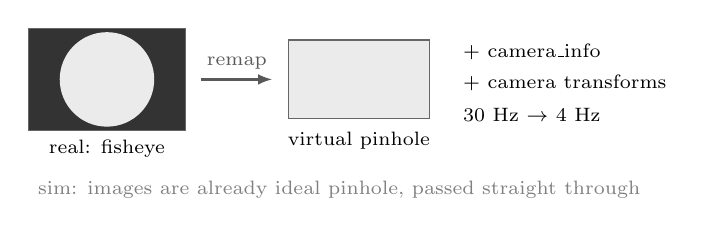
\begin{tikzpicture}[font=\scriptsize]
    \draw[black!60, fill=black!80] (0,0) rectangle (2.0,1.3);
    \fill[black!8] (1.0,0.65) circle (0.6);
    \node[below] at (1.0,0) {real: fisheye};
    \draw[arr] (2.2,0.65) -- node[above]{remap} (3.1,0.65);
    \draw[black!60, fill=black!8] (3.3,0.15) rectangle (5.1,1.15);
    \node[below] at (4.2,0.1) {virtual pinhole};
    \node[anchor=west] at (5.4,1.0) {$+$ camera\_info};
    \node[anchor=west] at (5.4,0.6) {$+$ camera transforms};
    \node[anchor=west] at (5.4,0.2) {30 Hz $\rightarrow$ 4 Hz};
    \node[anchor=west, text=black!50] at (0,-0.75) {sim: images are already ideal pinhole, passed straight through};
  \end{tikzpicture}}%
  {Builds the calibration messages and camera transforms from the same files VINS
   reads, so there is one source of truth.}
  {The recordings hold only compressed images --- no calibration messages, no
   camera transforms --- and RTAB-Map will not start without both.}
  {compressed stereo, 30 Hz}
  {rectified pair + calibration, 4 Hz; camera TF}
  {A wrong calibration or transform puts the map in the wrong place; the real-rig remap narrows the view.}
  {shim start-up line in \repo{launch.log} (rate, field of view); the TF tree}
  \src{4 Hz because RTAB-Map looks at one frame per second (RTAB-3); 30 Hz would only cost bandwidth.}
\end{frame}

% ---------------------------------------------------------------- RTAB-2
\begin{frame}{1.4.2 \;RTAB-2 \;Odometry in: RTAB-Map borrows the front end's motion}
  \hl{RTAB2}
  \compbody{\rtabstrip}{rtabc}{%
  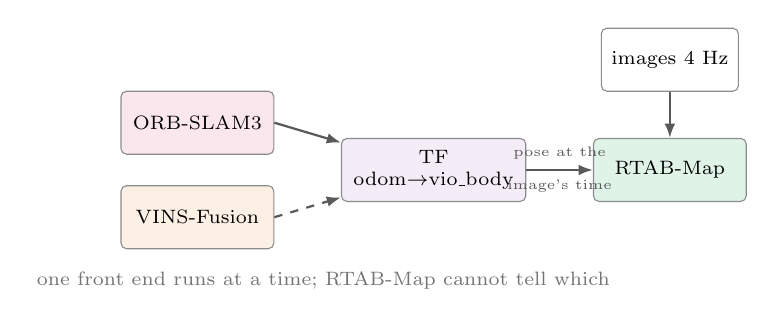
\begin{tikzpicture}[font=\scriptsize]
    \node[box, text width=18mm, fill=orbc!12] (o) at (0,0.7) {ORB-SLAM3};
    \node[box, text width=18mm, fill=vinsc!12] (v) at (0,-0.5) {VINS-Fusion};
    \node[box, text width=22mm, fill=dpose!10] (tf) at (3.0,0.1) {TF\\odom$\rightarrow$vio\_body};
    \node[box, text width=18mm, fill=rtabc!15] (r) at (6.0,0.1) {RTAB-Map};
    \node[box, text width=16mm] (im) at (6.0,1.5) {images 4 Hz};
    \draw[arr] (o.east) -- (tf); \draw[arr, dashed] (v.east) -- (tf);
    \draw[arr] (tf) -- node[above, font=\tiny]{pose at the} node[below, font=\tiny]{image's time} (r);
    \draw[arr] (im) -- (r);
    \node[text=black!55] at (1.6,-1.3) {one front end runs at a time; RTAB-Map cannot tell which};
  \end{tikzpicture}}%
  {Looks up the pose on TF at each image's timestamp (waiting up to 5 s), and
   pairs it with that image.}
  {RTAB-Map is a back end: it does not measure motion itself, it borrows it from
   whichever front end is running.}
  {TF odom$\rightarrow$vio\_body + images, 4 Hz}
  {synchronised (images, pose) pairs}
  {If the front end lags, images wait for their pose or are dropped.}
  {TF-wait warnings in \repo{launch.log}; node count in the database}
  \src{Reading the pose from TF rather than an odometry topic is a measured choice: on the same bag the topic route kept 3 nodes, TF kept 28.}
\end{frame}

% ---------------------------------------------------------------- RTAB-3
\begin{frame}{1.4.3 \;RTAB-3 \;New node: which places get remembered \;(mapping only)}
  \hl{RTAB3}\res{\R{10}{}}
  \compbody{\rtabstrip}{rtabc}{%
  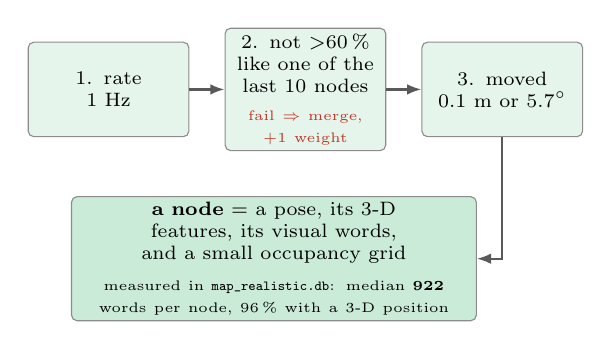
\begin{tikzpicture}[font=\scriptsize, g/.style={box, fill=rtabc!12, text width=19mm, minimum height=12mm}]
    \node[g] (g1) at (0,0)   {1. rate\\1 Hz};
    \node[g] (g2) at (2.5,0) {2. not $>$60\,\% like one of the last 10 nodes\\[2pt]
                              {\tiny\color{bad}fail $\Rightarrow$ merge, $+1$ weight}};
    \node[g] (g3) at (5.0,0) {3. moved\\0.1 m or 5.7$^\circ$};
    \foreach \a/\b in {g1/g2,g2/g3} \draw[arr] (\a) -- (\b);
    \node[box, text width=50mm, fill=rtabc!25] (n) at (2.1,-2.15)
      {\textbf{a node} = a pose, its 3-D features, its visual words, and a small occupancy grid\\[3pt]
       \mdseries\tiny measured in \repo{map_realistic.db}: median \textbf{922} words per node, 96\,\% with a 3-D position};
    \draw[arr] (g3.south) |- (n.east);
  \end{tikzpicture}}%
  {Three gates, in the library's own order: rate, then novelty, then motion.
   Novelty compares \emph{visual words} --- not pixels --- and only against the
   last 10 nodes, which are the ones the robot just drove past.}
  {A node is one remembered place. Too many and the map bloats; too few and
   places are missed on the way back.}
  {synchronised pairs, 4 Hz}
  {a new node --- only when the robot has moved}
  {Nodes too far apart: a place is missed on return. Standing still still raises a node's weight, because novelty is tested before motion.}
  {database \texttt{Node} table: count, weight, timestamps}
\end{frame}

% ---------------------------------------------------------------- RTAB-4
\begin{frame}{1.4.4 \;RTAB-4 \;Memory: short-term, working and long-term (no limit set)}
  \hl{RTAB4}
  \compbody{\rtabstrip}{rtabc}{%
  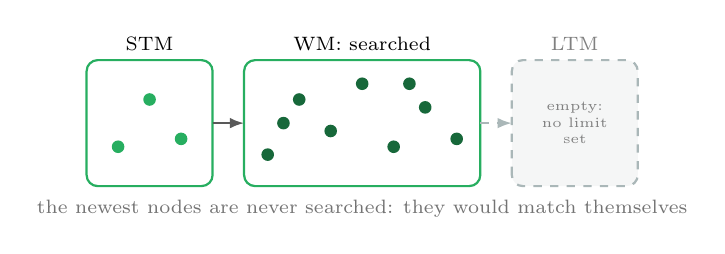
\begin{tikzpicture}[font=\scriptsize]
    \draw[rtabc, thick, rounded corners] (0,0) rectangle (1.6,1.6);  \node[above] at (0.8,1.6) {STM};
    \draw[rtabc, thick, rounded corners] (2.0,0) rectangle (5.0,1.6); \node[above] at (3.5,1.6) {WM: searched};
    \draw[offc, dashed, thick, rounded corners, fill=offc!12] (5.4,0) rectangle (7.0,1.6);
    \node[above, text=black!50] at (6.2,1.6) {LTM};
    \foreach \x/\y in {0.4/0.5,0.8/1.1,1.2/0.6} \node[pt=rtabc] at (\x,\y) {};
    \foreach \x/\y in {2.3/0.4,2.7/1.1,3.1/0.7,3.5/1.3,3.9/0.5,4.3/1.0,4.7/0.6,2.5/0.8,4.1/1.3}
      \node[pt=rtabc!60!black] at (\x,\y) {};
    \node[text=black!50, align=center, font=\tiny] at (6.2,0.8) {empty:\\no limit\\set};
    \draw[arr] (1.6,0.8) -- (2.0,0.8);
    \draw[darr, offc] (5.0,0.8) -- (5.4,0.8);
    \node[below, text=black!55] at (3.5,-0.05) {the newest nodes are never searched: they would match themselves};
  \end{tikzpicture}}%
  {LTM is where nodes go when a time or memory budget is exceeded, and come
   back from near a revisit. Ours: library default 0 = no limit, so LTM stays
   empty. It must stay so: read-only localisation cannot be combined with it.}
  {Recognition compares against every node it is allowed to search, so it slows
   as the map grows. RTAB-Map keeps only part of the map ``awake''.}
  {new nodes}
  {the nodes stage 1 searches (WM)}
  {Nothing at today's map size. Recognition time grows, because nothing is moved out.}
  {database \texttt{Info} / \texttt{Statistics}: working-memory size, timings}
\end{frame}

% ---------------------------------------------------------------- RTAB-5
\begin{frame}{1.4.5 \;RTAB-5 \;Detect (stage 1): which remembered place does this look like?}
  \hl{RTAB5}\res{\R{11}{}}
  \compbody{\rtabstrip}{rtabc}{%
  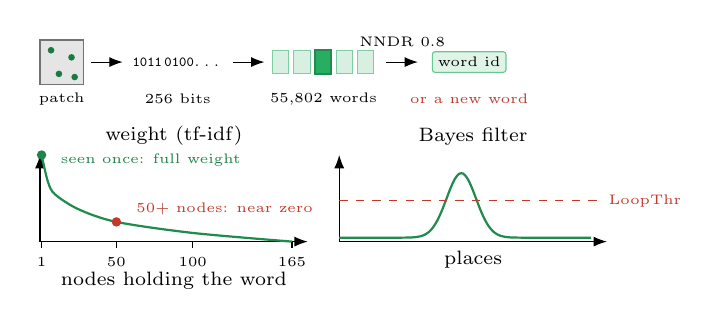
\begin{tikzpicture}[font=\scriptsize]
    % ---- top row: where a visual word comes from (quantisation)
    \begin{scope}[yshift=2.28cm, font=\tiny]
      \draw[black!55, fill=black!10] (0,-0.28) rectangle (0.55,0.28);
      \foreach \a/\b in {0.14/0.15,0.40/0.06,0.24/-0.15,0.44/-0.19}
        \fill[rtabc!70!black] (\a,\b) circle (0.042);
      \node at (0.275,-0.47) {patch};
      \draw[-{Latex}] (0.65,0) -- (1.05,0);
      \node[font=\tiny\ttfamily] at (1.75,0) {1011\,0100$\dots$};
      \node at (1.75,-0.47) {256 bits};
      \draw[-{Latex}] (2.45,0) -- (2.85,0);
      \foreach \i in {0,...,4} \draw[draw=rtabc!60, fill=rtabc!18] (2.95+\i*0.27,-0.15) rectangle ++(0.21,0.3);
      \draw[draw=rtabc!80!black, fill=rtabc, line width=0.7pt] (2.95+2*0.27,-0.15) rectangle ++(0.21,0.3);
      \node at (3.6,-0.47) {55{,}802 words};
      \draw[-{Latex}] (4.40,0) -- (4.80,0);
      \node at (4.60,0.26) {NNDR 0.8};
      \node[draw=rtabc!70, fill=rtabc!15, rounded corners=1pt, inner sep=2pt] at (5.45,0) {word id};
      \node[text=bad] at (5.45,-0.47) {or a new word};
    \end{scope}
    % ---- bottom row: scoring (unchanged)
    % tf-idf: a word's weight against how many nodes hold it (measured, 165 nodes)
    \draw[-{Latex}] (0,0) -- (3.4,0); \draw[-{Latex}] (0,0) -- (0,1.10);
    \draw[thick, rtabc!80!black] plot[smooth] coordinates
      {(0.02,1.10) (0.10,0.76) (0.19,0.60) (0.49,0.41) (0.97,0.25) (1.94,0.11) (3.20,0.00)};
    \fill[good] (0.02,1.10) circle (0.06);
    \fill[bad]  (0.97,0.25) circle (0.06);
    \node[font=\tiny, text=good, anchor=west] at (0.14,1.03) {seen once: full weight};
    \node[font=\tiny, text=bad, anchor=west] at (1.10,0.42) {50$+$ nodes: near zero};
    \foreach \x/\l in {0.02/1, 0.97/50, 1.94/100, 3.20/165}
      {\draw (\x,0) -- (\x,-0.08); \node[font=\tiny, below] at (\x,-0.08) {\l};}
    \node[below] at (1.7,-0.26) {nodes holding the word};
    \node[above] at (1.7,1.10) {weight (tf-idf)};
    \draw[-{Latex}] (3.8,0) -- (7.2,0); \draw[-{Latex}] (3.8,0) -- (3.8,1.10);
    \draw[thick, rtabc!80!black] plot[smooth, domain=0:3.2, samples=60]
      ({3.8+\x},{0.05+0.82*exp(-((\x-1.55)^2)/0.07)});
    \draw[dashed, hlc] (3.8,0.52) -- (7.1,0.52) node[right, font=\tiny, text=hlc]{LoopThr};
    \node[below] at (5.5,0) {places};
    \node[above] at (5.5,1.10) {Bayes filter};
  \end{tikzpicture}}%
  {A word's weight falls with how many nodes hold it: 44{,}716 of ours sit in
   one node, 467 in fifty or more.}
  {Checking every node's geometry is too slow. Stage 1 looks only at \emph{which}
   words appear: cheap, at any map size.}
  {the new node's words}
  {one candidate place --- or ``new place''}
  {Lookalike places score high: repeated racks share most of their words.}
  {hypotheses in \repo{launch.log}; read by \repo{script/exp4_rtabmap_gating.py}}
\end{frame}

% ---------------------------------------------------------------- RTAB-6
\begin{frame}{1.4.6 \;RTAB-6 \;Verify (stage 2): is it really the same place?}
  \hl{RTAB6}\res{\R{11}{}}
  \compbody{\rtabstrip}{rtabc}{%
  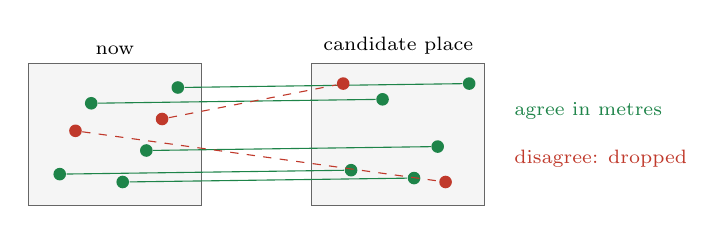
\begin{tikzpicture}[font=\scriptsize]
    \draw[black!60, fill=black!4] (0,0) rectangle (2.2,1.8); \node[above] at (1.1,1.8) {now};
    \draw[black!60, fill=black!4] (3.6,0) rectangle (5.8,1.8); \node[above] at (4.7,1.8) {candidate place};
    \foreach \a/\b in {0.4/0.4, 0.8/1.3, 1.5/0.7, 1.9/1.5, 1.2/0.3} {
      \node[pt=good] (L) at (\a,\b) {}; \node[pt=good] (R) at (3.7+\a,\b+0.05) {};
      \draw[good] (L) -- (R);}
    \foreach \a/\b/\c/\d in {0.6/0.95/5.3/0.3, 1.7/1.1/4.0/1.55} {
      \node[pt=bad] (L) at (\a,\b) {}; \node[pt=bad] (R) at (\c,\d) {};
      \draw[bad, dashed] (L) -- (R);}
    \node[anchor=west, text=good] at (6.05,1.2) {agree in metres};
    \node[anchor=west, text=bad] at (6.05,0.6) {disagree: dropped};
  \end{tikzpicture}}%
  {Fit one rigid transform to the matched features (RANSAC) and count how many
   agree within 0.1\,m in 3-D. At least 20: the link is accepted.}
  {Words cannot tell two identical aisles apart. Geometry can: the same place
   must line up in 3-D.}
  {the candidate (RTAB-5)}
  {an accepted link + transform --- or rejection}
  {Identical objects give a geometrically consistent wrong match.}
  {``Not enough inliers'' lines in \repo{launch.log}; \repo{exp4_rtabmap_gating.py}}
  \src{Ours: \texttt{Vis/EstimationType 0} --- points must agree \emph{in metres}, not merely reproject (library default 1). The ICP check (\texttt{Reg/Strategy 2}) is off.}
\end{frame}

% ---------------------------------------------------------------- RTAB-7
\begin{frame}{1.4.7 \;RTAB-7 \;Graph optimisation: make the whole map agree}
  \hl{RTAB7}
  \compbody{\rtabstrip}{rtabc}{%
  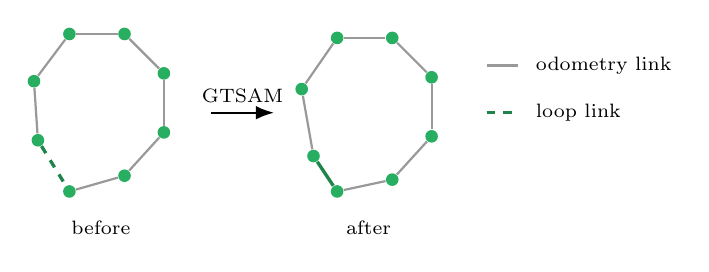
\begin{tikzpicture}[font=\scriptsize]
    \foreach \i/\x/\y in {0/0/0, 1/0.7/0.2, 2/1.2/0.75, 3/1.2/1.5, 4/0.7/2.0, 5/0/2.0, 6/-0.45/1.4, 7/-0.4/0.65}
      \node[pt=rtabc] (a\i) at (\x,\y) {};
    \foreach \i [evaluate=\i as \n using int(\i+1)] in {0,...,6} \draw[black!40, thick] (a\i) -- (a\n);
    \draw[good, very thick, dashed] (a7) -- (a0);
    \node[below] at (0.4,-0.25) {before};
    \draw[-{Latex}, thick] (1.8,1.0) -- (2.6,1.0) node[midway, above]{GTSAM};
    \foreach \i/\x/\y in {0/3.4/0, 1/4.1/0.15, 2/4.6/0.7, 3/4.6/1.45, 4/4.1/1.95, 5/3.4/1.95, 6/2.95/1.3, 7/3.1/0.45}
      \node[pt=rtabc] (b\i) at (\x,\y) {};
    \foreach \i [evaluate=\i as \n using int(\i+1)] in {0,...,6} \draw[black!40, thick] (b\i) -- (b\n);
    \draw[good, very thick] (b7) -- (b0);
    \node[below] at (3.8,-0.25) {after};
    \draw[black!40, thick] (5.3,1.6) -- ++(0.4,0); \node[anchor=west] at (5.8,1.6) {odometry link};
    \draw[good, very thick, dashed] (5.3,1.0) -- ++(0.4,0); \node[anchor=west] at (5.8,1.0) {loop link};
  \end{tikzpicture}}%
  {Nodes are poses; links are odometry steps, loop links and proximity links.
   GTSAM moves the nodes until every link is satisfied as well as possible.}
  {A new loop link means the drift built up along the way must be spread over
   the whole graph.}
  {links: odometry, loop, proximity}
  {optimised node poses}
  {A wrong link that is self-consistent passes the guard.}
  {``Rejecting all added loop closures'' in \repo{launch.log}; node poses in the database}
  \src{Guard: a link stretched more than 10$\times$ its expected error rejects the new closures (\texttt{RGBD/OptimizeMaxError}; library default 3). In localise mode the graph is frozen.}
\end{frame}

% ---------------------------------------------------------------- RTAB-8
\begin{frame}{1.4.8 \;RTAB-8 \;Map assembly: from node grids to the planner's map}
  \hl{RTAB8}\res{\R{10}{}, \R{12}{}, \R{13}{}}
  \compbody{\rtabstrip}{rtabc}{%
  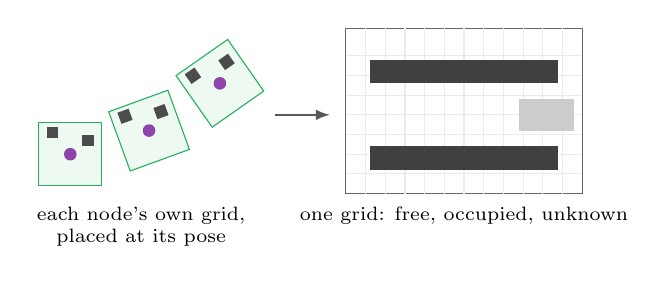
\begin{tikzpicture}[font=\scriptsize]
    \foreach \x/\y/\r in {0/0/0, 1.0/0.3/20, 1.9/0.9/35} {
      \begin{scope}[shift={(\x,\y)}, rotate=\r]
        \draw[rtabc, fill=rtabc!8] (-0.4,-0.4) rectangle (0.4,0.4);
        \fill[black!70] (0.15,0.1) rectangle ++(0.15,0.15);
        \fill[black!70] (-0.3,0.2) rectangle ++(0.15,0.15);
        \node[pt=dpose] at (0,0) {};
      \end{scope}}
    \node[below, align=center] at (0.9,-0.55) {each node's own grid,\\placed at its pose};
    \draw[arr] (2.6,0.5) -- (3.3,0.5);
    \draw[black!60, fill=white] (3.5,-0.5) rectangle (6.5,1.6);
    \foreach \x in {3.75,4.0,...,6.25} \draw[black!8] (\x,-0.5) -- (\x,1.6);
    \foreach \y in {-0.25,0.0,...,1.35} \draw[black!8] (3.5,\y) -- (6.5,\y);
    \fill[black!75] (3.8,0.9) rectangle (6.2,1.2);
    \fill[black!75] (3.8,-0.2) rectangle (6.2,0.1);
    \fill[black!20] (5.7,0.3) rectangle (6.4,0.7);
    \node[below] at (5.0,-0.55) {one grid: free, occupied, unknown};
  \end{tikzpicture}}%
  {Each node's small grid is built once, from its stereo depth. The global grid
   places them all at their optimised poses, on 0.05\,m cells.}
  {Nav2 plans on a single occupancy grid: free, occupied or unknown, cell by cell.}
  {each node's grid + its pose}
  {\texttt{/map}, sent once (latched)}
  {A node placed wrong leaves obstacles that nothing later removes.}
  {exported grid vs ground-truth map (Experiment 2A scoring)}
\end{frame}

% ---------------------------------------------------------------- RTAB-9
\begin{frame}{1.4.9 \;RTAB-9 \;Output: the correction, and the gate we added}
  \hl{RTAB9}\res{\R{10}{}, \R{13}{}}
  \compbody{\rtabstrip}{rtabc}{\includegraphics{rtab9_bound.png}}%
  {Every correction RTAB-Map proposed in six runs. Accepted only if step
   \emph{and} turn fit the box. 63 accepted, all right; 5 refused: one
   wrong-aisle match, a big step with almost no turn.}
  {In localise mode RTAB-Map's output is a correction, map$\rightarrow$odom. A wrong
   one moves the robot to the wrong aisle instantly.}
  {\texttt{/localization\_pose}, $\approx$1 Hz}
  {TF map$\rightarrow$odom, 20 Hz}
  {A refused true correction lets the pose drift until a fix is accepted.}
  {\repo{gate_verdicts.csv}: verdict, size, allowance; \repo{localize_*.csv}}
  \src{Refusing is cheap: the front end drifts at most \textbf{0.76 m over 21--152 m}. Eight refusals in a row and the gate concedes.}
\end{frame}

% ---------------------------------------------------------------- config
\begin{frame}{1.4.10 \;RTAB-Map configuration}
  \centering
  \adjustbox{max width=\textwidth, max height=0.80\textheight}{%
  \begin{tabular}{l l l l l}
    \toprule
    & Parameter & Ours & Library & What it means \\
    \midrule
    RTAB-1 & \textcolor{ourc}{shim rate} & 4 Hz & --- & images handed to RTAB-Map per second \\
    RTAB-3 & \texttt{Rtabmap/DetectionRate} & 1 Hz & 1 Hz & frames considered per second \\
           & \texttt{RGBD/LinearUpdate} / \texttt{AngularUpdate} & 0.1 m / 0.1 rad & same & move this much to make a node \\
           & \texttt{Mem/RehearsalSimilarity} & 0.6 & 0.6 & merge a node this similar to a recent one \\
           & \texttt{Vis/MaxFeatures} / \texttt{Kp/MaxFeatures} & 1000 / 500 & same & features / words kept per node \\
    RTAB-4 & \texttt{Rtabmap/TimeThr} / \texttt{MemoryThr} & 0 / 0 & 0 / 0 & 0 = no limit; required by read-only localise \\
    RTAB-5 & \texttt{Rtabmap/LoopThr} & 0.11 & 0.11 & stage-1 threshold \\
    RTAB-6 & \texttt{Vis/EstimationType} & \textcolor{bad}{\textbf{0}} & 1 & verify in metres (3-D to 3-D) \\
           & \texttt{Vis/MinInliers} / \texttt{InlierDistance} & 20 / 0.1 m & same & stage-2 acceptance \\
           & \texttt{Reg/Strategy} & 0 & 0 & no ICP check \\
    RTAB-7 & \texttt{RGBD/OptimizeMaxError} & \textcolor{bad}{\textbf{10}} & 3 & graph guard; 3 rejects a drifting VIO's closures \\
    RTAB-9 & \textcolor{ourc}{\texttt{localize\_delay\_s}} & 5 s & --- & hold RTAB-Map back at start \\
           & \textcolor{ourc}{correction gate} & 1.5 m $+$ 0.02 m/m, 8$^\circ$ $+$ 0.1$^\circ$/m & --- & largest correction accepted \\
    \bottomrule
  \end{tabular}}
  \par\vspace{0.5em}
  \scriptsize\color{black!65}
  \textcolor{bad}{\textbf{Red}}: the only two values that differ from the RTAB-Map 0.23 library.
  \textcolor{ourc}{\textbf{Amber}}: added by this project.
  \src{\repo{vslam_navigation/launch/rtabmap.launch.py}; values as printed in each run's \repo{launch.log}; defaults from rtabmap 0.23 \repo{Parameters.h}}
\end{frame}

% =============================================================================
% 1.5  NAV2
% Sources: vslam_navigation/params/nav2_sim.yaml, launch/navigate_sim.launch.py,
% scripts/pose_gate.py; the Experiment 2B run logs for what was switched on.
% =============================================================================
\section{1.5 Nav2}

\begin{frame}{1.5 \;Nav2: plan on the prior map, drive on the localised pose}
  \centering
  \adjustbox{max width=\textwidth, max height=0.70\textheight}{%
  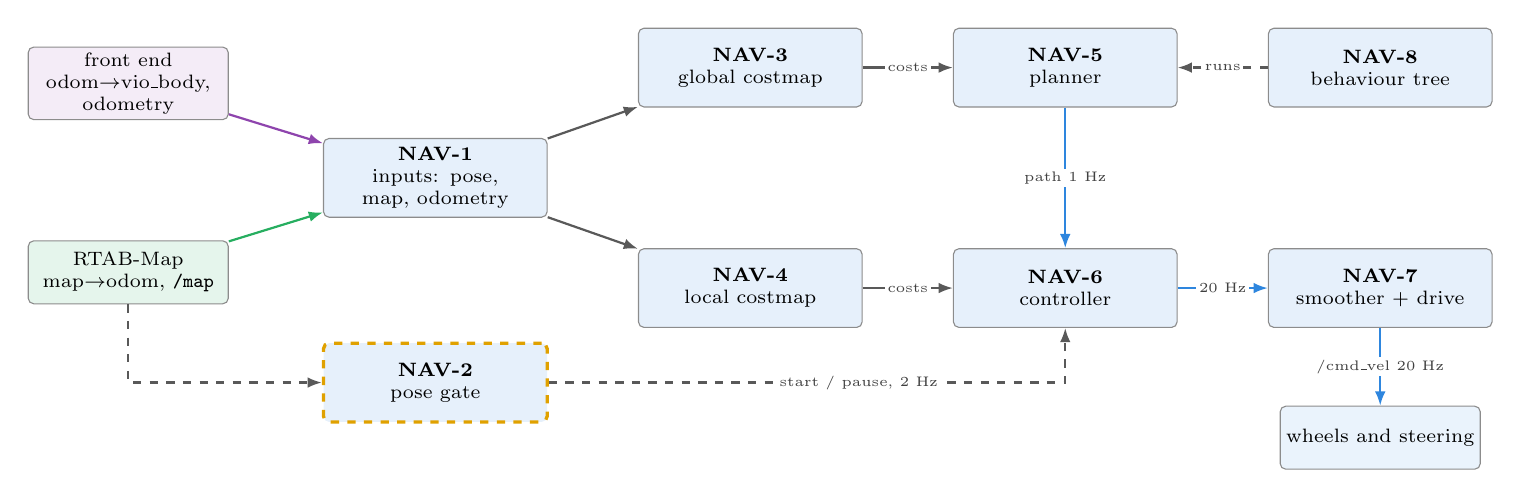
\begin{tikzpicture}[font=\scriptsize,
      cb/.style={box, fill=navc!12, text width=27mm, minimum height=10mm}]
    \node[box, text width=24mm, fill=dpose!10] (fe) at (0,1.2)  {front end\\odom$\rightarrow$vio\_body, odometry};
    \node[box, text width=24mm, fill=rtabc!12] (rt) at (0,-1.2) {RTAB-Map\\map$\rightarrow$odom, \texttt{/map}};
    \node[cb, NAV1] (n1) at (3.9,0)    {\textbf{NAV-1}\\inputs: pose, map, odometry};
    \node[cb, ours, NAV2] (n2) at (3.9,-2.6) {\textbf{NAV-2}\\pose gate};
    \node[cb, NAV3] (n3) at (7.9,1.4)  {\textbf{NAV-3}\\global costmap};
    \node[cb, NAV4] (n4) at (7.9,-1.4) {\textbf{NAV-4}\\local costmap};
    \node[cb, NAV5] (n5) at (11.9,1.4) {\textbf{NAV-5}\\planner};
    \node[cb, NAV6] (n6) at (11.9,-1.4) {\textbf{NAV-6}\\controller};
    \node[cb, NAV7] (n7) at (15.9,-1.4) {\textbf{NAV-7}\\smoother + drive};
    \node[cb, NAV8] (n8) at (15.9,1.4) {\textbf{NAV-8}\\behaviour tree};
    \node[box, text width=24mm, fill=dcmd!10] (cmd) at (15.9,-3.3) {wheels and steering};
    \draw[arr, dpose] (fe) -- (n1); \draw[arr, rtabc] (rt) -- (n1);
    \draw[arr] (n1) -- (n3); \draw[arr] (n1) -- (n4);
    \draw[arr] (n3) -- node[rate]{costs} (n5);
    \draw[arr] (n4) -- node[rate]{costs} (n6);
    \draw[arr, dcmd] (n5) -- node[rate]{path 1 Hz} (n6);
    \draw[arr, dcmd] (n6) -- node[rate]{20 Hz} (n7);
    \draw[arr, dcmd] (n7) -- node[rate]{/cmd\_vel 20 Hz} (cmd);
    \draw[darr] (n8) -- node[rate]{runs} (n5);
    \draw[darr] (rt.south) |- (n2.west);
    \draw[darr] (n2.east) -| node[rate, pos=0.3]{start / pause, 2 Hz} (n6.south);
  \end{tikzpicture}}
  \par\vspace{0.3em}
  \small Nav2 is the standard ROS~2 navigation stack. It \textbf{never sees
  ground truth}: it plans on the grid RTAB-Map built and drives on the pose the
  front end and RTAB-Map produce together. Anything wrong upstream arrives here
  as a planning input.
  \src{\repo{vslam_navigation/params/nav2_sim.yaml}; \repo{launch/navigate_sim.launch.py}}
\end{frame}

% ---------------------------------------------------------------- NAV-1
\begin{frame}{1.5.1 \;NAV-1 \;Inputs: where the robot is, what the world is, how fast it moves}
  \hl{NAV1}
  \compbody{\navstrip}{navc}{%
  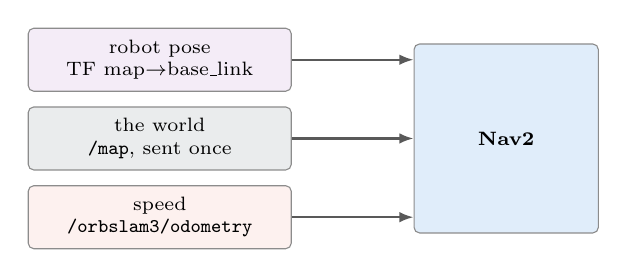
\begin{tikzpicture}[font=\scriptsize]
    \node[box, text width=22mm, fill=navc!15, minimum height=24mm] (n) at (4.4,0) {\textbf{Nav2}};
    \node[box, text width=32mm, fill=dpose!10] (a) at (0,1.0)  {robot pose\\TF map$\rightarrow$base\_link};
    \node[box, text width=32mm, fill=dmap!10]  (b) at (0,0)    {the world\\\texttt{/map}, sent once};
    \node[box, text width=32mm, fill=dimg!8]   (c) at (0,-1.0) {speed\\\texttt{/orbslam3/odometry}};
    \foreach \x in {a,b,c} \draw[arr] (\x.east) -- (n.west |- \x.east);
  \end{tikzpicture}}%
  {Pose comes from the frame chain of 1.1; the map from RTAB-Map's database;
   speed from the front end's own odometry. Nothing publishes \texttt{/odom} here.}
  {To plan, Nav2 needs three things: where the robot is, what the world looks
   like, and how fast it is moving.}
  {TF, \texttt{/map}, odometry}
  {--- (used by NAV-3 to NAV-7)}
  {A transform older than 0.30\,s stops the controller; a pose jump moves the robot on the costmap.}
  {the TF tree; Nav2 transform-timeout warnings}
\end{frame}

% ---------------------------------------------------------------- NAV-2
\begin{frame}{1.5.2 \;NAV-2 \;Pose gate: is the localisation sound enough to drive on?}
  \hl{NAV2}\res{\R{10}{}}
  \compbody{\navstrip}{navc}{%
  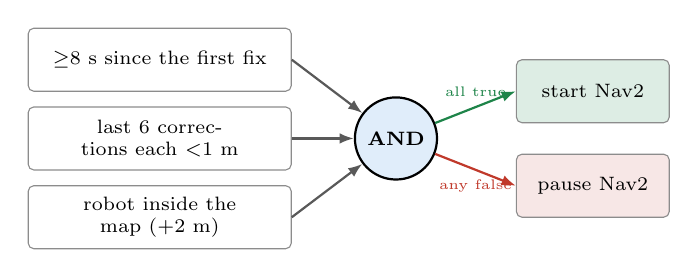
\begin{tikzpicture}[font=\scriptsize]
    \node[box, text width=32mm] (c1) at (0,1.0)  {$\ge$8 s since the first fix};
    \node[box, text width=32mm] (c2) at (0,0)    {last 6 corrections each $<$1 m};
    \node[box, text width=32mm] (c3) at (0,-1.0) {robot inside the map ($+$2 m)};
    \node[circle, draw, thick, fill=navc!15, minimum size=9mm, font=\scriptsize\bfseries] (and) at (3.0,0) {AND};
    \foreach \x in {c1,c2,c3} \draw[arr] (\x.east) -- (and);
    \node[box, text width=18mm, fill=good!15] (go) at (5.5,0.6)  {start Nav2};
    \node[box, text width=18mm, fill=bad!12]  (st) at (5.5,-0.6) {pause Nav2};
    \draw[arr, good] (and) -- node[above, font=\tiny]{all true} (go.west);
    \draw[arr, bad]  (and) -- node[below, font=\tiny]{any false} (st.west);
  \end{tikzpicture}}%
  {Three checks, twice a second, combined into one \texttt{/localization\_ok}.
   That is why Nav2's \texttt{autostart} is false: this node starts it.}
  {Nav2 trusts whatever pose it is given, and a confident pose from RTAB-Map is
   not necessarily a right one.}
  {map$\rightarrow$odom, map$\rightarrow$base\_link, the prior's extent}
  {\texttt{/localization\_ok}, 2 Hz; start / pause}
  {A wrong pose that stays steady passes; a right pose that jumps once pauses driving.}
  {\texttt{/localization\_ok}, \texttt{/localization\_status}; the gate's log file}
\end{frame}

% ---------------------------------------------------------------- NAV-3
\begin{frame}{1.5.3 \;NAV-3 \;Global costmap: a price for every cell of the map}
  \hl{NAV3}\res{\R{12}{}}
  \compbody{\navstrip}{navc}{%
  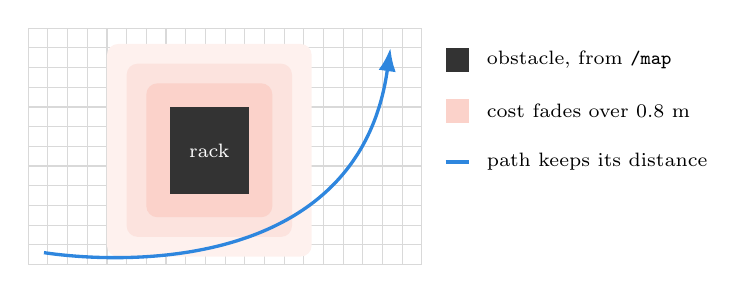
\begin{tikzpicture}[font=\scriptsize]
    \draw[black!15, step=0.25] (0,0) grid (5,3);
    \foreach \d/\c in {0.8/10,0.55/20,0.3/32}
      \fill[plancol!\c, rounded corners=4pt] (1.8-\d,0.9-\d) rectangle (2.8+\d,2.0+\d);
    \fill[black!80] (1.8,0.9) rectangle (2.8,2.0);
    \node[text=white] at (2.3,1.45) {rack};
    \draw[navc, very thick, -{Latex}] (0.2,0.15) .. controls (1.2,0.0) and (4.2,-0.1) .. (4.6,2.75);
    \fill[black!80] (5.3,2.45) rectangle ++(0.3,0.3); \node[anchor=west] at (5.7,2.6) {obstacle, from \texttt{/map}};
    \fill[plancol!32] (5.3,1.8) rectangle ++(0.3,0.3);  \node[anchor=west] at (5.7,1.95) {cost fades over 0.8 m};
    \draw[navc, very thick] (5.3,1.3) -- ++(0.3,0);      \node[anchor=west] at (5.7,1.3) {path keeps its distance};
  \end{tikzpicture}}%
  {Three layers: the prior map (static), live obstacles, and inflation, which
   makes cells near obstacles expensive so paths keep their distance.}
  {The planner needs a price for every cell: free, near something, or blocked.}
  {\texttt{/map} + live points + pose}
  {costmap, 15$\times$22 m, 0.05 m cells, 2 Hz}
  {Phantom obstacles in the prior block real aisles. Unknown cells cannot be planned through.}
  {the published costmap; Experiment 2A map scoring}
  \src{The live obstacle layer reads RTAB-Map's \texttt{/local\_grid\_obstacle}, published only with \texttt{local\_grid:=true}.
       Every Experiment 2B run logged it \textbf{off}, so the costmaps held the prior map only.}
\end{frame}

% ---------------------------------------------------------------- NAV-4
\begin{frame}{1.5.4 \;NAV-4 \;Local costmap: a window that travels with the robot}
  \hl{NAV4}\res{not measured (\R{14}{})}
  \compbody{\navstrip}{navc}{%
  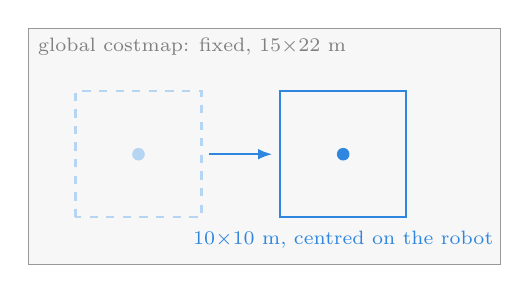
\begin{tikzpicture}[font=\scriptsize]
    \draw[black!40, fill=black!3] (0,0) rectangle (6,3);
    \node[anchor=north west, text=black!50] at (0,3) {global costmap: fixed, 15$\times$22 m};
    \draw[navc!35, thick, dashed] (0.6,0.6) rectangle (2.2,2.2); \node[pt=navc!35] at (1.4,1.4) {};
    \draw[navc, thick] (3.2,0.6) rectangle (4.8,2.2); \node[pt=navc] at (4.0,1.4) {};
    \draw[arr, navc] (2.3,1.4) -- (3.1,1.4);
    \node[below, text=navc] at (4.0,0.55) {10$\times$10 m, centred on the robot};
  \end{tikzpicture}}%
  {Same three layers as NAV-3, but only around the robot, rolling as it drives;
   this is what the controller checks against.}
  {The controller needs a fresh picture of the robot's immediate surroundings.}
  {same layers as NAV-3}
  {costmap, 10$\times$10 m around the robot, 2 Hz}
  {If the pose jumps, the window --- and what is in it --- jumps with it.}
  {the local costmap topic}
  \src{It rolls because map$\rightarrow$odom can jump. A fixed window in the odom frame was safe only in the ground-truth setup, where that link never moved.}
\end{frame}

% ---------------------------------------------------------------- NAV-5
\begin{frame}{1.5.5 \;NAV-5 \;Planner: a path a car can actually drive}
  \hl{NAV5}\res{not measured (\R{14}{})}
  \compbody{\navstrip}{navc}{%
  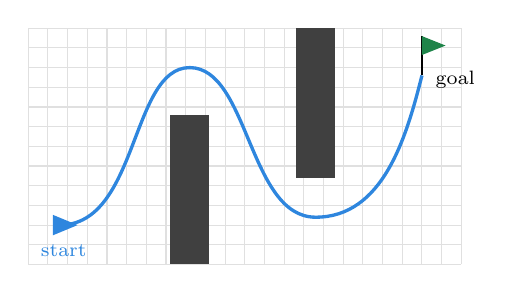
\begin{tikzpicture}[font=\scriptsize]
    \draw[black!12, step=0.25] (0,0) grid (5.5,3);
    \fill[black!75] (1.8,0) rectangle (2.3,1.9);
    \fill[black!75] (3.4,1.1) rectangle (3.9,3);
    \draw[navc, very thick] (0.4,0.5) .. controls (1.4,0.5) and (1.3,2.5) .. (2.05,2.5)
                                    .. controls (2.8,2.5) and (2.8,0.6) .. (3.65,0.6)
                                    .. controls (4.5,0.6) and (4.8,1.6) .. (5.0,2.4);
    \node[isosceles triangle, fill=navc, minimum size=2.6mm, inner sep=0pt] at (0.4,0.5) {};
    \node[below, text=navc] at (0.45,0.38) {start};
    \draw[thick] (5.0,2.4) -- (5.0,2.9);
    \fill[good] (5.0,2.9) -- (5.3,2.78) -- (5.0,2.66) -- cycle;
    \node[right] at (5.05,2.35) {goal};
  \end{tikzpicture}}%
  {Smac Hybrid-A*: searches position \emph{and} heading (72 headings) with
   forward-only arcs, turning radius at least 0.75 m. Refuses unknown cells.}
  {The robot is car-like: it cannot turn on the spot, so a shortest straight-line
   path is often not drivable.}
  {pose, global costmap, goal}
  {a drivable path, replanned at 1 Hz}
  {No path when unknown space blocks the route; an outdated map gives a path through something real.}
  {planner log; per-goal result in \repo{outcome.json}}
\end{frame}

% ---------------------------------------------------------------- NAV-6
\begin{frame}{1.5.6 \;NAV-6 \;Controller: follow the path, 20 times a second}
  \hl{NAV6}\res{not measured (\R{14}{})}
  \compbody{\navstrip}{navc}{%
  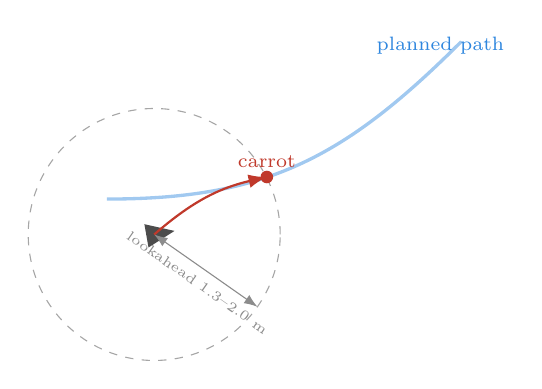
\begin{tikzpicture}[font=\scriptsize]
    \draw[navc!45, very thick] (0,0) .. controls (2,0) and (3,0.5) .. (4.5,2.0);
    \coordinate (r) at (0.6,-0.45);
    \coordinate (c) at (2.03,0.28);
    \draw[black!35, dashed] (r) circle (1.6);
    \node[isosceles triangle, fill=black!70, minimum size=3mm, inner sep=0pt, rotate=10] at (r) {};
    \node[pt=hlc] at (c) {};
    \node[above, text=hlc] at (c) {carrot};
    \draw[hlc, thick, -{Latex}] (r) to[bend left=14] (c);
    \draw[{Latex}-{Latex}, black!45] (r) -- node[below, sloped, font=\tiny]{lookahead 1.3--2.0 m} ($(r)+(-35:1.6)$);
    \node[anchor=west, text=navc] at (3.3,1.95) {planned path};
  \end{tikzpicture}}%
  {Regulated Pure Pursuit: pick a ``carrot'' on the path 1.3--2.0 m ahead and
   steer the arc that reaches it. 1.5 m/s, slower on tight curves; no reversing.}
  {A path is a line on a map; the wheels need a speed and a turn rate, many times a second.}
  {path, local costmap, odometry}
  {speed + turn rate, 20 Hz}
  {With collision checking off, it does not stop for a newly seen obstacle by itself.}
  {\texttt{/cmd\_vel}; progress checker (must move 0.5 m in 15 s)}
  \src{Collision checking is off (in tuning it vetoed the controller's own corner-cutting); avoidance comes from the 1 Hz replan.}
\end{frame}

% ---------------------------------------------------------------- NAV-7
\begin{frame}{1.5.7 \;NAV-7 \;Velocity smoother and drive: turn a command into wheel motion}
  \hl{NAV7}\res{not measured (\R{14}{})}
  \compbody{\navstrip}{navc}{%
  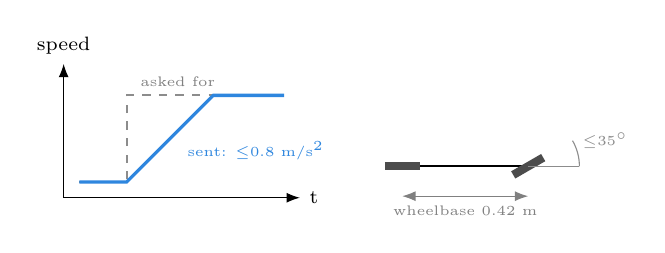
\begin{tikzpicture}[font=\scriptsize]
    \draw[-{Latex}] (0,0) -- (3.0,0) node[right]{t};
    \draw[-{Latex}] (0,0) -- (0,1.7) node[above]{speed};
    \draw[black!45, dashed, thick] (0.2,0.2) -- (0.8,0.2) -- (0.8,1.3) -- (2.8,1.3);
    \draw[navc, very thick] (0.2,0.2) -- (0.8,0.2) -- (1.9,1.3) -- (2.8,1.3);
    \node[text=black!50, font=\tiny, anchor=west] at (0.85,1.48) {asked for};
    \node[text=navc, font=\tiny, anchor=west] at (1.45,0.6) {sent: $\le$0.8 m/s$^2$};
    \begin{scope}[shift={(4.3,0.4)}]
      \draw[thick] (0,0) -- (1.6,0);
      \draw[line width=3pt, black!70] (-0.22,0) -- (0.22,0);
      \draw[line width=3pt, black!70, rotate around={30:(1.6,0)}] (1.38,0) -- (1.82,0);
      \draw[{Latex}-{Latex}, black!50] (0,-0.38) -- node[below, font=\tiny]{wheelbase 0.42 m} (1.6,-0.38);
      \draw[black!45] (1.6,0) -- (2.25,0);
      \draw[black!45] (2.25,0) arc (0:30:0.65) node[right, font=\tiny]{$\le$35$^\circ$};
    \end{scope}
  \end{tikzpicture}}%
  {Caps speed and acceleration, scaling all components together so the curve is
   kept; the Ackermann plugin turns speed + turn rate into wheel speed and steering.}
  {Raw commands can jump, and a real chassis has acceleration and steering limits.}
  {controller command, 20 Hz}
  {\texttt{/cmd\_vel}, 20 Hz $\rightarrow$ wheels and steering}
  {A turn sharper than the steering limit cannot be executed.}
  {\texttt{/cmd\_vel}; \repo{robot_gt.csv}: what the robot actually did}
\end{frame}

% ---------------------------------------------------------------- NAV-8
\begin{frame}{1.5.8 \;NAV-8 \;Behaviour tree: run the sequence, recover from failure}
  \hl{NAV8}\res{not measured (\R{14}{})}
  \compbody{\navstrip}{navc}{%
  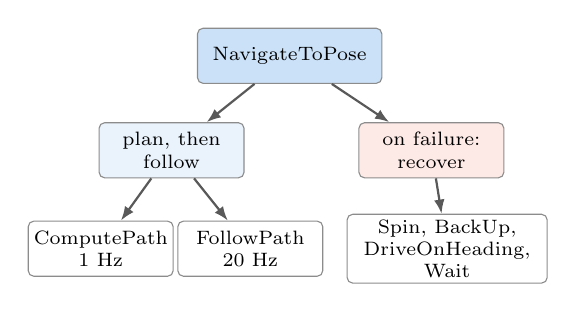
\begin{tikzpicture}[font=\scriptsize, t/.style={box, text width=17mm, minimum height=7mm}]
    \node[t, fill=navc!25, text width=22mm] (root) at (2.4,2.2) {NavigateToPose};
    \node[t, fill=navc!10] (seq) at (0.9,1.0) {plan, then follow};
    \node[t, fill=plancol!15] (rec) at (4.2,1.0) {on failure: recover};
    \node[t] (cp) at (0,-0.25) {ComputePath\\1 Hz};
    \node[t] (fp) at (1.9,-0.25) {FollowPath\\20 Hz};
    \node[t, text width=24mm] (rv) at (4.4,-0.25) {Spin, BackUp,\\DriveOnHeading, Wait};
    \draw[arr] (root) -- (seq); \draw[arr] (root) -- (rec);
    \draw[arr] (seq) -- (cp); \draw[arr] (seq) -- (fp); \draw[arr] (rec) -- (rv);
  \end{tikzpicture}}%
  {Nav2's default tree: replan once a second, follow the path, and on failure try
   a recovery before giving up on the goal.}
  {Something has to run the sequence: plan, follow, notice failure, recover, try again.}
  {goal(s) --- ours are poses of prior-map nodes}
  {calls to planner, controller, recoveries; a result per goal}
  {Recovery loops; the progress checker aborts a robot that has stopped moving.}
  {\repo{outcome.json}: per-goal result; the \texttt{bt\_navigator} log}
\end{frame}

% ---------------------------------------------------------------- config
\begin{frame}{1.5.9 \;Nav2 configuration}
  \centering
  \adjustbox{max width=\textwidth, max height=0.80\textheight}{%
  \begin{tabular}{l l l l}
    \toprule
    & Parameter & Value & What it means \\
    \midrule
    NAV-1 & \texttt{transform\_tolerance} & 0.30 s & oldest pose the stack accepts \\
          & \texttt{odom\_topic} & \texttt{/orbslam3/odometry} & speed comes from the front end \\
    NAV-2 & \textcolor{ourc}{\texttt{init\_ignore\_s}, stability, margin} & 8 s; 6 $\times$ $<$1 m; 2 m & the three checks \\
          & \texttt{autostart} & false & the pose gate starts Nav2 \\
    NAV-3 & global costmap & 15$\times$22 m fixed, 0.05 m, 2 Hz & planner's map \\
          & \texttt{inflation\_radius} / \texttt{cost\_scaling\_factor} & 0.80 m / 3.0 & how far, how fast cost fades \\
          & obstacle layer source & \texttt{/local\_grid\_obstacle} & \textcolor{bad}{off in Exp.~2B runs} \\
    NAV-4 & local costmap & 10$\times$10 m rolling, 0.05 m, 2 Hz & controller's window \\
    NAV-5 & planner & Smac Hybrid-A*, Dubins, 72 headings & forward-only arcs \\
          & \texttt{minimum\_turning\_radius} / \texttt{allow\_unknown} & 0.75 m / false & tightest turn; no unknown cells \\
          & \texttt{expected\_planner\_frequency} & 1 Hz & replanning rate \\
    NAV-6 & controller & Regulated Pure Pursuit, 20 Hz & follow the carrot \\
          & \texttt{desired\_linear\_vel} / lookahead & 1.5 m/s / 1.3--2.0 m & cruise speed, carrot distance \\
          & \texttt{use\_collision\_detection} & false & avoidance by replanning \\
          & goal checker & 1.0 m, any heading & when a goal counts as reached \\
    NAV-7 & smoother max / accel & 1.5 m/s, 1.0 rad/s / 0.8 m/s$^2$ & speed and acceleration caps \\
          & chassis & wheelbase 0.42 m, steering $\le$35$^\circ$ & what the wheels can do \\
    NAV-8 & progress checker & 0.5 m within 15 s & otherwise the goal is aborted \\
    \bottomrule
  \end{tabular}}
  \par\vspace{0.4em}
  \scriptsize\color{black!65}\textcolor{ourc}{\textbf{Amber}}: our pose gate's parameters. Simulation values; a real-rig file (\repo{nav2_real.yaml}) exists but has not been driven.
  \src{\repo{vslam_navigation/params/nav2_sim.yaml}; \repo{scripts/pose_gate.py}; Experiment 2B \repo{launch.log}}
\end{frame}

% =============================================================================
% RESULTS THROUGH THE ARCHITECTURE.  Only findings with a mechanism inside a
% block are here; score tables stay in the experiment notes.  Every number is
% quoted from docs/report/insights/experiment_{1,3,4}/experiment_N.tex.
% Finding IDs R1..R13 are stable: the component slides and the index link to
% them by label.
% =============================================================================
\section{Results through the architecture}

\newcommand{\twostrips}[2]{%
  {\centering\adjustbox{scale=0.66}{\parbox{\textwidth}{#1}}\par
   \vspace{-0.15em}\adjustbox{scale=0.66}{\parbox{\textwidth}{#2}}\par}\vspace{0.1em}}

% ---------------------------------------------------------------- map
\begin{frame}{2.0 \;Where the results land}
  \centering\scriptsize
  Each finding below is a place where a result can be explained by one block.
  Click an R-number to jump.\par\vspace{0.4em}
  \adjustbox{max width=\textwidth}{%
  \begin{tabular}{@{}l l l@{\qquad}l l l@{}}
    \toprule
    & Block & Finding & & Block & Finding \\
    \midrule
    \hyperlink{R1}{\textbf{R1}} & ORB-1 & faster front end, same accuracy &
    \hyperlink{R8}{\textbf{R8}} & ORB-1/2, VINS-1/2 & real rig: better images, slower robot \\
    \hyperlink{R2}{\textbf{R2}} & ORB-7, ORB-8 & false loop closure on a repeated object &
    \hyperlink{R9}{\textbf{R9}} & ORB-1, 5, 6 & three rules for reading ORB numbers \\
    \hyperlink{R3}{\textbf{R3}} & ORB-6, ORB-8 & gravity needs a turn; tilt becomes height &
    \hyperlink{R10}{\textbf{R10}} & RTAB-5, RTAB-6 & words propose, geometry disposes \\
    \hyperlink{R4}{\textbf{R4}} & ORB-6 & a robot standing still resets the map &
    \hyperlink{R11}{\textbf{R11}} & RTAB-3/8/9, NAV-2 & the first second poisons two layers \\
    \hyperlink{R5}{\textbf{R5}} & VINS-1 vs ORB-3 & blank wall: VINS starves, ORB bridges &
    \hyperlink{R12}{\textbf{R12}} & RTAB-8 $\rightarrow$ NAV-3 & poses are fine, the grid is not \\
    \hyperlink{R6}{\textbf{R6}} & VINS-1, VINS-4 & fisheye rim: dividing by $z$ explodes &
    \hyperlink{R13}{\textbf{R13}} & RTAB-9 & the pose is as good as the map \\
    \hyperlink{R7}{\textbf{R7}} & ORB-3, VINS-1/4 & the one mover that hurts: ahead, same way &
    \hyperlink{R14}{\textbf{R14}} & Nav2, \ldots & what is not measured yet \\
    \bottomrule
  \end{tabular}}
  \par\vspace{0.6em}
  \begin{tabular}{@{}l@{\quad}l@{}}
    \textbf{Experiment 1} & localisation accuracy: ORB-SLAM3 vs VINS-Fusion, sim (4 bags) and real rig (realv6/7) \\
    \textbf{Experiment 3} & map quality: RTAB-Map occupancy grid against the world \\
    \textbf{Experiment 4} & relocalisation in a prior map: RTAB-Map + ORB-SLAM3, 6 hand-driven runs \\
  \end{tabular}
\end{frame}

% ---------------------------------------------------------------- R1
\begin{frame}[label=R1]{R1 \;ORB-1 \;A faster front end buys frames, not accuracy}
  \hl{ORB1}\orbstrip\par\vspace{0.2em}
  \finding{orbc}{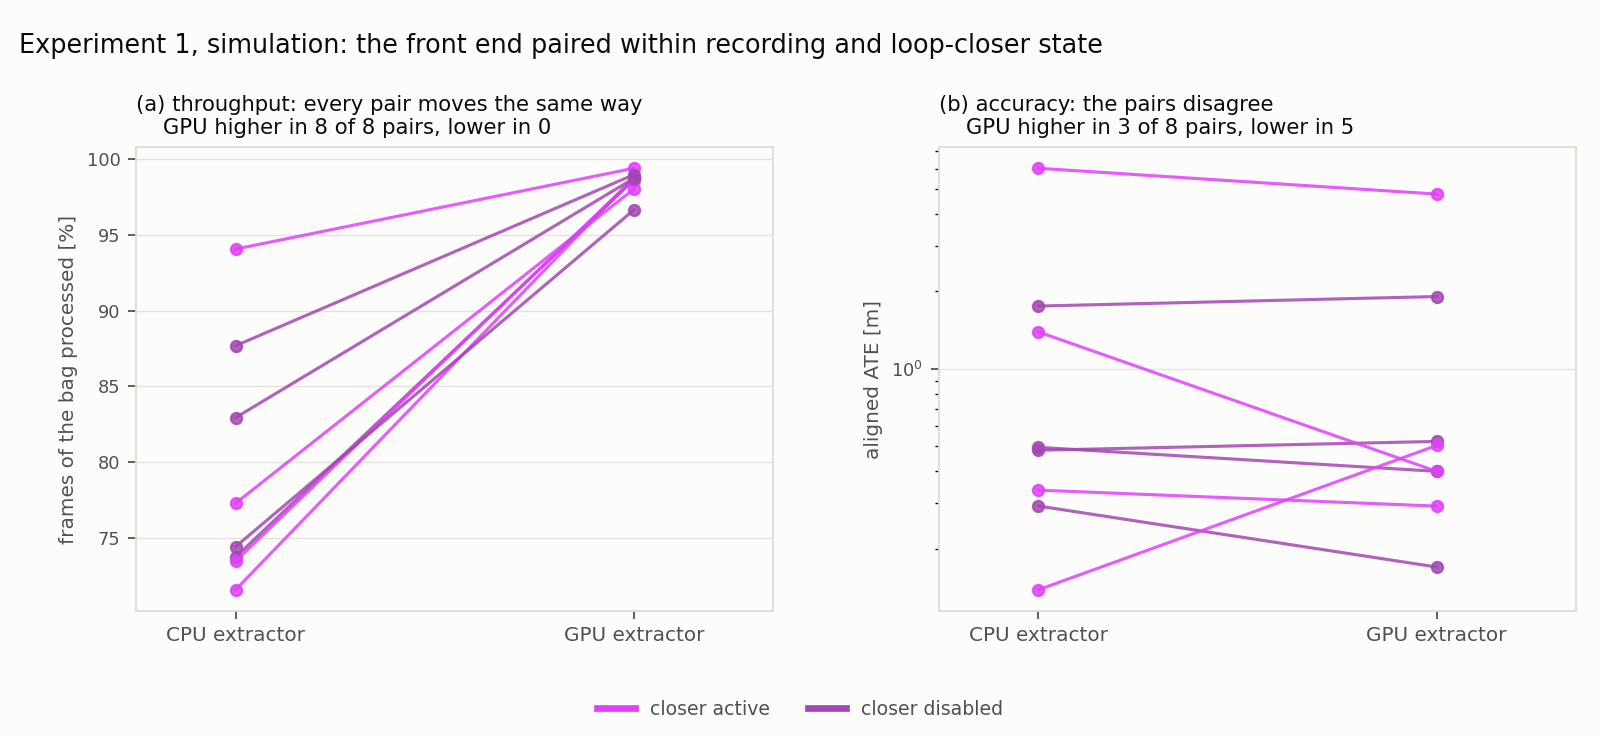
\includegraphics{exp1_frontend_pairs.png}}%
  {Swap only the extractor (CPU $\rightarrow$ GPU), same bag, same closer state.
   \textbf{Sim:} frames kept rise in 8 of 8 pairs (72--94\,\% $\rightarrow$ 97--99\,\%);
   ATE rises in 3, falls in 5.
   \textbf{Robot:} 6 of 6 pairs, ATE within 0.02\,m.}%
  {ORB-1 only decides how many frames reach ORB-3. The robot moves
   0.28\,m/s, so even the CPU's 9\,Hz is 3\,cm per frame: nothing is missed.
   The large errors come from discrete events further down the chain
   (\R{2}{}, \R{3}{}).}%
  {one run per cell; ORB-SLAM3 repeats spread up to 0.28\,m (\R{9}{}), wider than most gaps.}
\end{frame}

% ---------------------------------------------------------------- R2
\begin{frame}[label=R2]{R2 \;ORB-7 + ORB-8 \;A false loop closure on a repeated object}
  \hl{ORB7}\hl{ORB8}\orbstrip\par\vspace{0.2em}
  \finding{orbc}{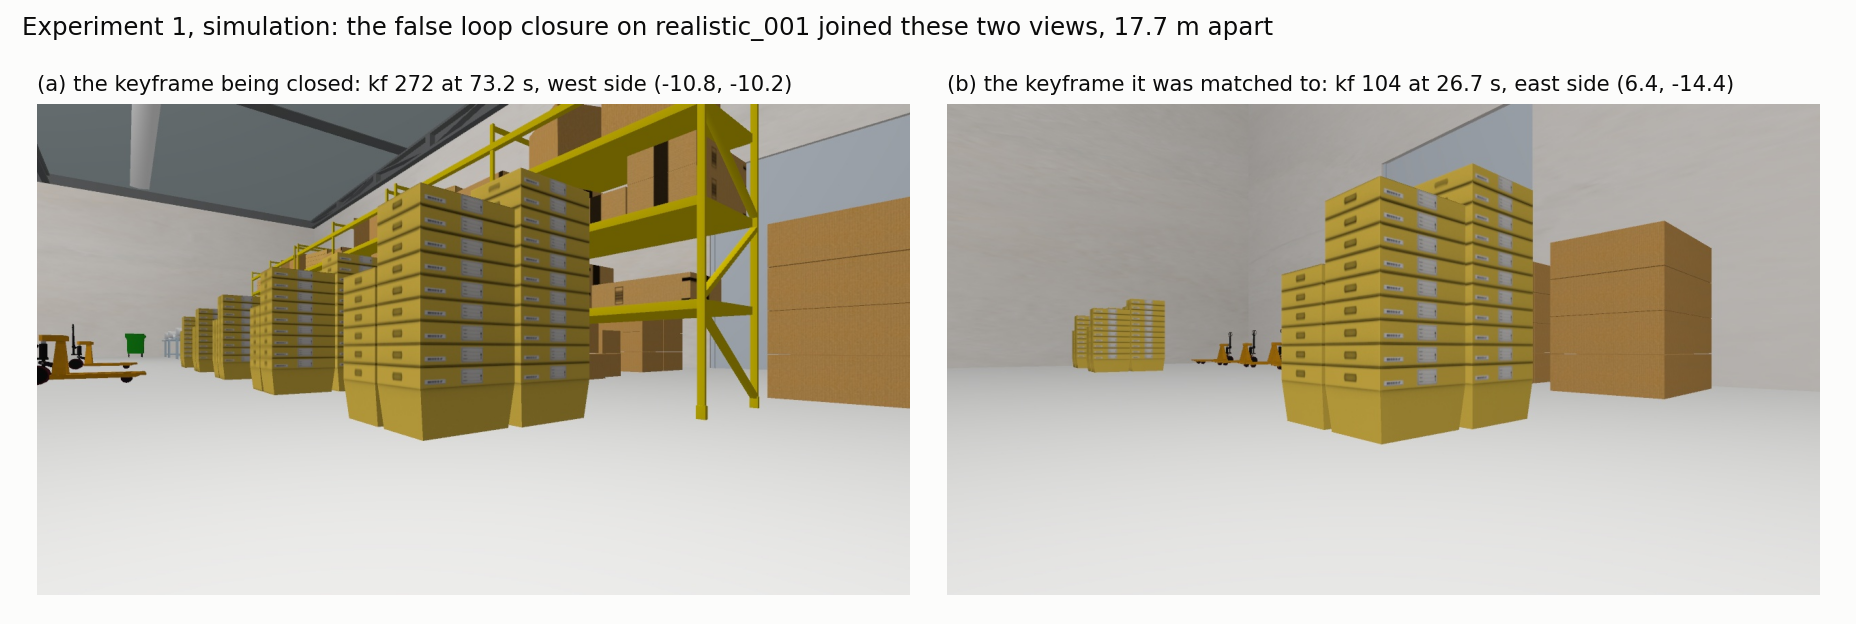
\includegraphics{exp1_false_closure.png}}%
  {Static I layout, \textbf{73.2\,s}: both front ends accept one closure,
   correction 14.7\,m (CPU) / 13.3\,m (GPU). The run ends 6.0 / 4.8\,m off;
   with the closer off: 0.50 / 0.40\,m.
   \textbf{Robot:} one loop-closing repeat took a \textbf{36.4\,m} closure, ended 10.7\,m off.}%
  {ORB-7 matched two keyframes 17.7\,m apart: same box-stack, so same
   words, and the geometric check passes because the objects
   \emph{are} identical. ORB-8 then bends the whole map. Nothing asks whether
   14\,m is plausible after 0.5\,m of drift.}%
  {diagnosed, not fixed. A correction bound like our RTAB-9 gate (\R{13}{}) is untested on ORB-8.}
\end{frame}

% ---------------------------------------------------------------- R3
\begin{frame}[label=R3]{R3 \;ORB-6 \;Gravity is found only while the robot turns}
  \hl{ORB6}\hl{ORB8}\orbstrip\par\vspace{0.2em}
  \finding{orbc}{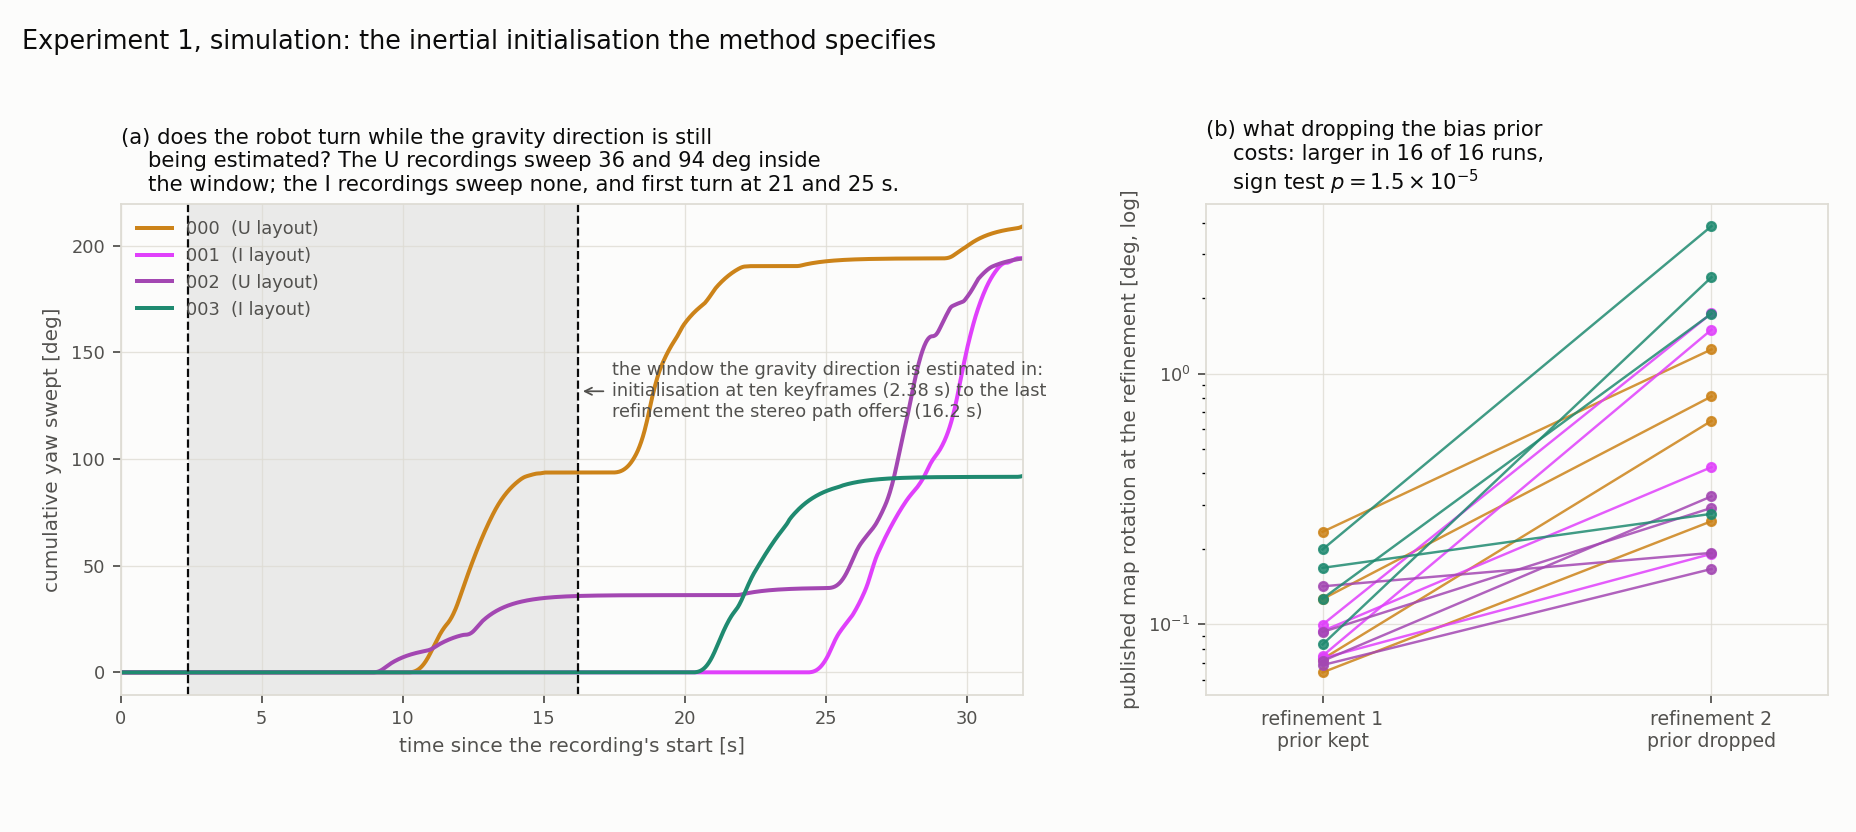
\includegraphics{exp1_imu_init.png}}%
  {In the init window (2.4--16.2\,s) the U routes turn 36--94$^\circ$, the I
   routes \textbf{0$^\circ$}. Tilt left over: 0.24--0.72$^\circ$ (U) vs
   up to 3.7$^\circ$ (I). On the I traffic bag the closer-off runs climb
   4.7--5.1\,m; with the closer on, 0.6--1.4\,m.}%
  {ORB-6 solves gravity direction and accelerometer bias together; they
   separate only if the body rotates. Drive straight for 16\,s and gravity
   stays tilted, with no later re-estimate on the stereo path. A tilted floor
   turns distance into height. Only a closure (ORB-8) pulls it back.}%
  {layout and opening move are confounded (2 routes vs 2). Test: an I-layout bag that turns in its first 15\,s.}
\end{frame}

% ---------------------------------------------------------------- R4
\begin{frame}[label=R4]{R4 \;ORB-6 \;A robot standing still at the start resets the map}
  \hl{ORB6}\orbstrip\par\vspace{0.2em}
  \finding{orbc}{%
  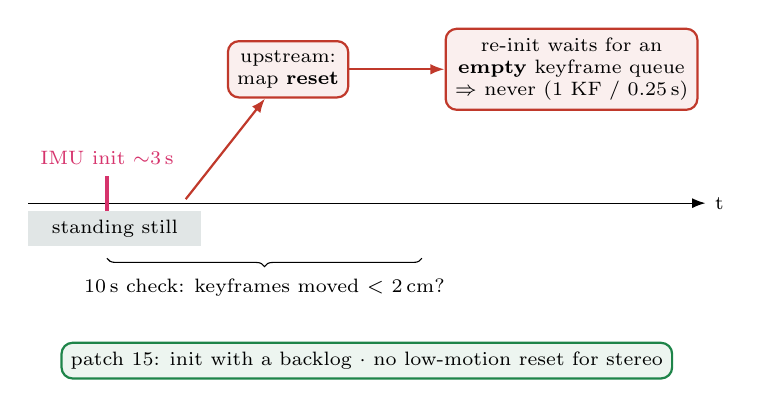
\begin{tikzpicture}[font=\scriptsize]
    \fill[offc!35] (0,-0.55) rectangle (2.2,-0.1); \node at (1.1,-0.33) {standing still};
    \draw[-{Latex}] (0,0) -- (8.6,0) node[right]{t};
    \draw[orbc, very thick] (1.0,-0.1) -- (1.0,0.35) node[above, text=orbc]{IMU init $\sim$3\,s};
    \draw[decorate, decoration={brace, amplitude=3pt, mirror}] (1.0,-0.7) -- (5.0,-0.7)
      node[midway, below=4pt]{10\,s check: keyframes moved $<$ 2\,cm?};
    \node[draw=bad, thick, rounded corners, align=center, fill=bad!8] (rs) at (3.3,1.7)
      {upstream:\\map \textbf{reset}};
    \draw[arr, bad] (2.0,0.05) -- (rs);
    \node[draw=bad, thick, rounded corners, align=center, fill=bad!8] (re) at (6.9,1.7)
      {re-init waits for an\\\textbf{empty} keyframe queue\\$\Rightarrow$ never (1 KF / 0.25\,s)};
    \draw[arr, bad] (rs) -- (re);
    \node[draw=good, thick, rounded corners, align=center, fill=good!8] at (4.3,-2.0)
      {patch 15: init with a backlog $\cdot$ no low-motion reset for stereo};
  \end{tikzpicture}}%
  {Robot recordings realv7, upstream: the IMU stayed uninitialised for most
   of 9 of 12 runs. With patch 15: IMU initialises at 2.8--4.7\,s in every
   run; 13 of 16 runs need no reset; floor tilt 0.2--2.8$^\circ$.}%
  {The upstream rule is written for hand-held cameras that move from the
   first second. A robot waiting at its start pose satisfies ``too little
   motion'' and gets reset; the re-try then starves behind ORB-5's
   keyframe queue.}%
  {patch 15 makes the runs scorable; it does \emph{not} make them more accurate (matches / splits / wins over three bags).}
\end{frame}

% ---------------------------------------------------------------- R5
\begin{frame}[label=R5]{R5 \;VINS-1 vs ORB-3 \;At a blank wall VINS starves and ORB bridges}
  \hl{VINS1}\hl{VINS4}\hl{ORB2}\hl{ORB3}\twostrips{\vinsstrip}{\orbstrip}
  \finding{vinsc}{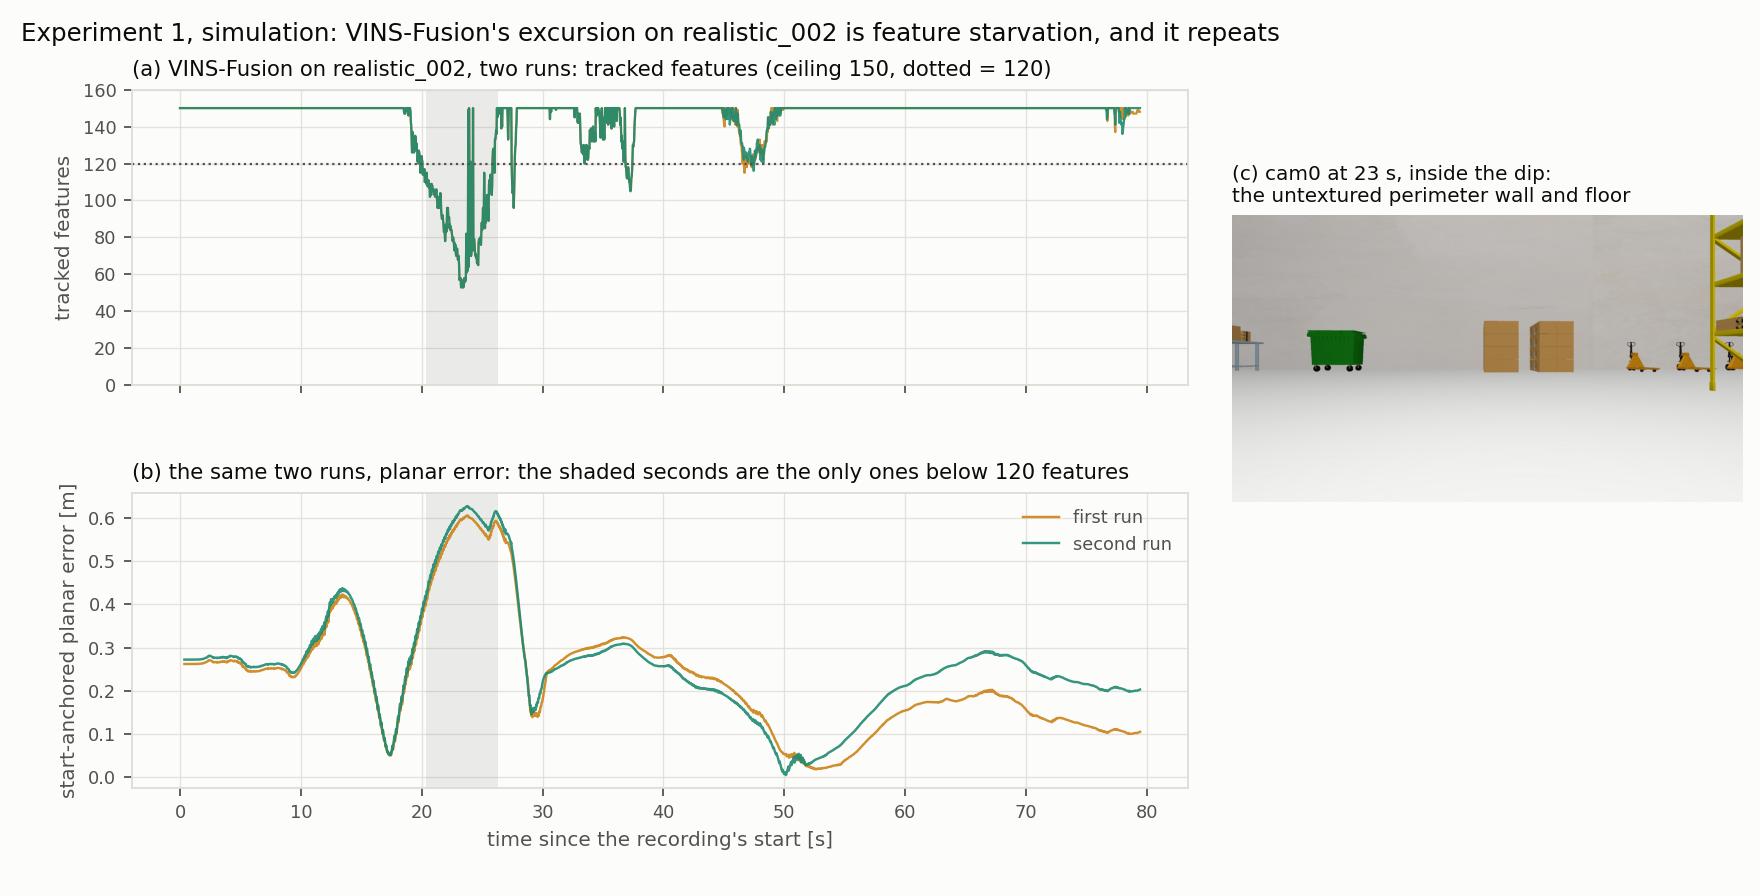
\includegraphics{exp1_vins_starvation.png}}%
  {U traffic bag, east aisle, 20--26\,s: VINS features 150 $\rightarrow$
   \textbf{53}, error +0.18\,m. A repeat run gives the same dip in the same
   second, within 6\,mm. ORB at a blank wall: 500 $\rightarrow$ $\sim$110 points
   for under 1\,s, no step.}%
  {VINS-1 can only keep corners that exist; blank wall + blank floor leave
   nothing to follow for 7\,s, and VINS-4 drifts. ORB-3 passes the same kind
   of wall in one second because ORB-2's IMU prediction carries it. Stereo
   depth held (92\,\%): it is the tracker, not the depth.}%
  {low-feature seconds are 8--20\,\% of a run: this explains VINS's \emph{excursions}, not its ATE. It cannot happen on the robot (\R{8}{}).}
\end{frame}

% ---------------------------------------------------------------- R6
\begin{frame}[label=R6]{R6 \;VINS-1 \;On a fisheye, dividing by depth explodes at the rim}
  \hl{VINS1}\hl{VINS4}\vinsstrip\par\vspace{0.2em}
  \finding{vinsc}{%
  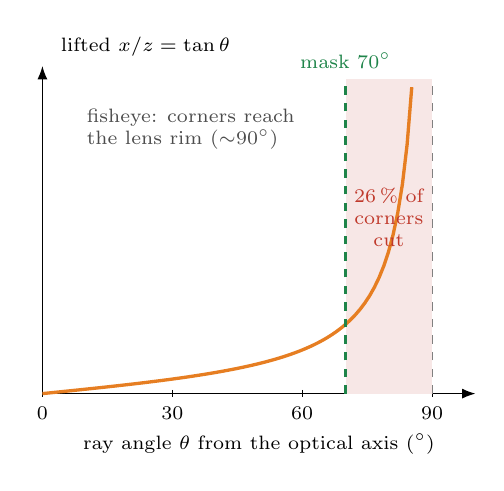
\begin{tikzpicture}[font=\scriptsize, x=0.055cm, y=0.32cm]
    \draw[-{Latex}] (0,0) -- (100,0);
    \node at (50,-2.0) {ray angle $\theta$ from the optical axis ($^\circ$)};
    \draw[-{Latex}] (0,0) -- (0,13);
    \node[anchor=south west] at (2,13) {lifted $x/z = \tan\theta$};
    \foreach \t in {0,30,60,90} \draw (\t,0.15) -- (\t,-0.15) node[below]{\t};
    \fill[bad!12] (70,0) rectangle (90,12.5);
    \draw[very thick, vinsc, domain=0:85.3, samples=80] plot (\x,{tan(\x)});
    \draw[dashed, good, thick] (70,0) -- (70,12.5) node[above, text=good]{mask 70$^\circ$};
    \draw[dashed, black!50] (90,0) -- (90,12.5);
    \node[text=bad, align=center] at (80,7) {26\,\% of\\corners\\cut};
    \node[align=left, text=black!70, anchor=west] at (8,10.5) {fisheye: corners reach\\the lens rim ($\sim$90$^\circ$)};
  \end{tikzpicture}}%
  {Robot, before the fix: VINS diverged on every recording, to $10^8$\,m on
   realv7\_001 (``parallax'' 6\,740\,px). After: three valid runs,
   0.37--0.68\,m, no reset; still 1.6--1.9$\times$ behind ORB.}%
  {VINS-1 turns each point into $(x/z,\,y/z)$. Near 90$^\circ$, $z\!\to\!0$: a
   corner on the rim lands thousands of units out and poisons VINS-4. Second
   fault: \texttt{estimate\_extrinsic} 1 let VINS-4 ``refine'' the stereo
   baseline away; now 0.}%
  {ORB uses the same lens model but never divides by $z$. The model also stops being monotonic at 109.3$^\circ$: real, but that band is black.}
\end{frame}

% ---------------------------------------------------------------- R7
\begin{frame}[label=R7]{R7 \;ORB-3 + VINS-1 \;The one mover that hurts: close, ahead, same way}
  \hl{ORB3}\hl{VINS1}\hl{VINS4}\twostrips{\orbstrip}{\vinsstrip}
  \finding{orbc}{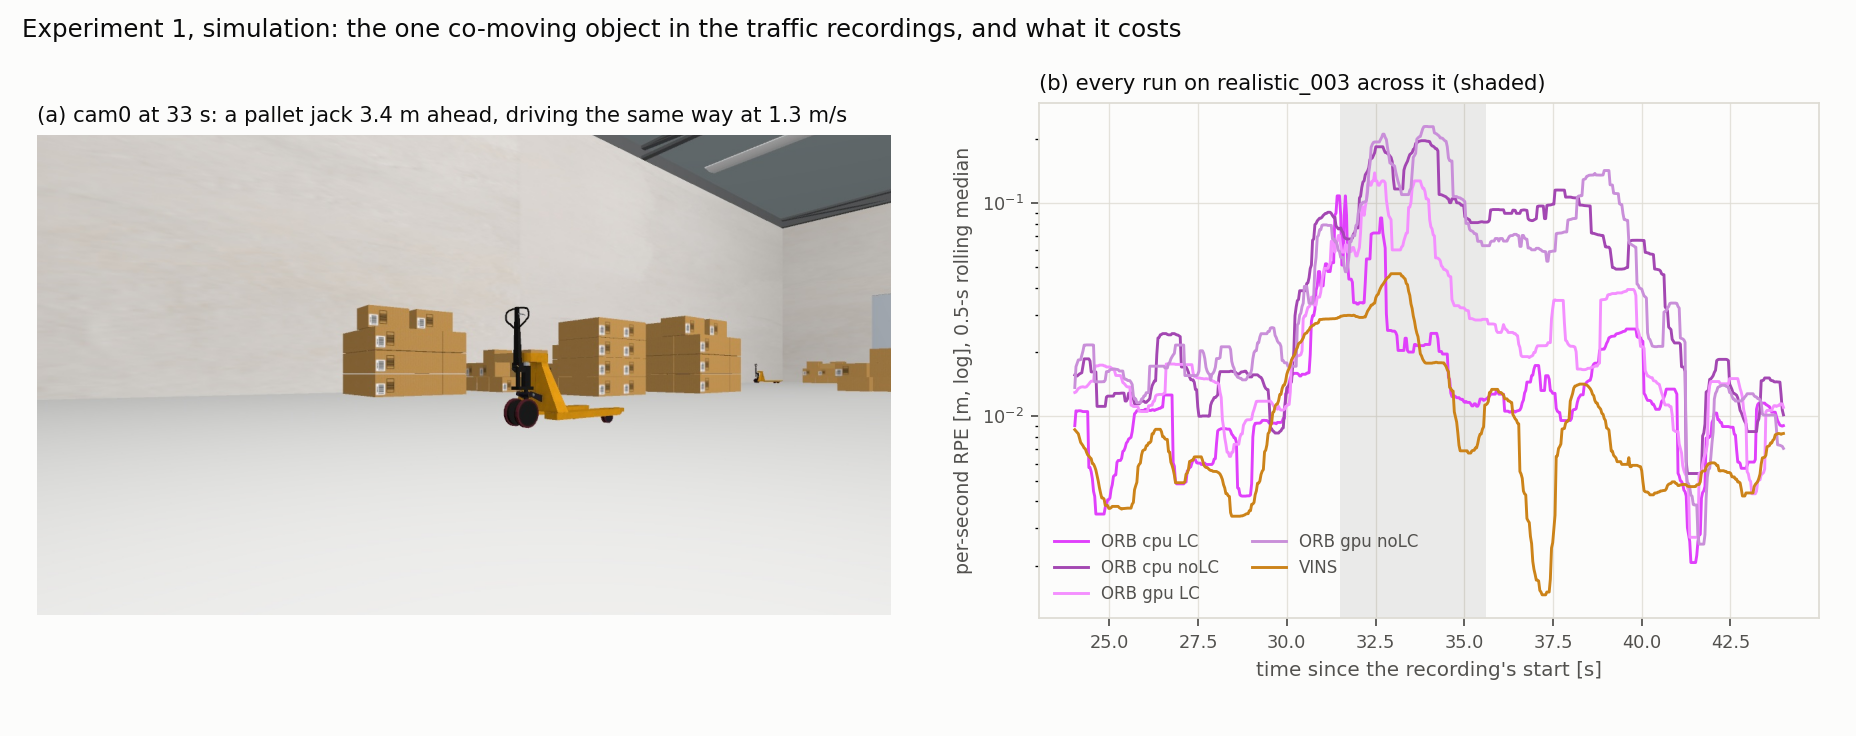
\includegraphics{exp1_jack_ahead.png}}%
  {I traffic bag, 31.5--35.6\,s: a pallet jack 3.4\,m ahead at 1.3\,m/s, the
   robot at 1.56. Error per second $\times$2--7.7 (ORB), $\times$3 (VINS);
   total step only $-0.03$ to $+0.09$\,m. Movers merely in view or crossing:
   \textbf{no cost}.}%
  {ORB-3 and VINS-4 drop points whose reprojection disagrees with the
   estimated motion (VINS-1's F-test is off in our fork). A co-moving object
   barely moves in the image, so its points pass as static structure.
   6--20\,m away the same jack did nothing.}%
  {one 4-second episode in 117\,s. Supports the project hypothesis in this one case, not ``movers degrade the estimate'' in general.}
\end{frame}

% ---------------------------------------------------------------- R8
\begin{frame}[label=R8]{R8 \;ORB-1/2 + VINS-1/2 \;Real rig: better images, slower robot}
  \hl{ORB1}\hl{ORB2}\hl{VINS1}\hl{VINS2}\twostrips{\orbstrip}{\vinsstrip}
  \finding{sysc}{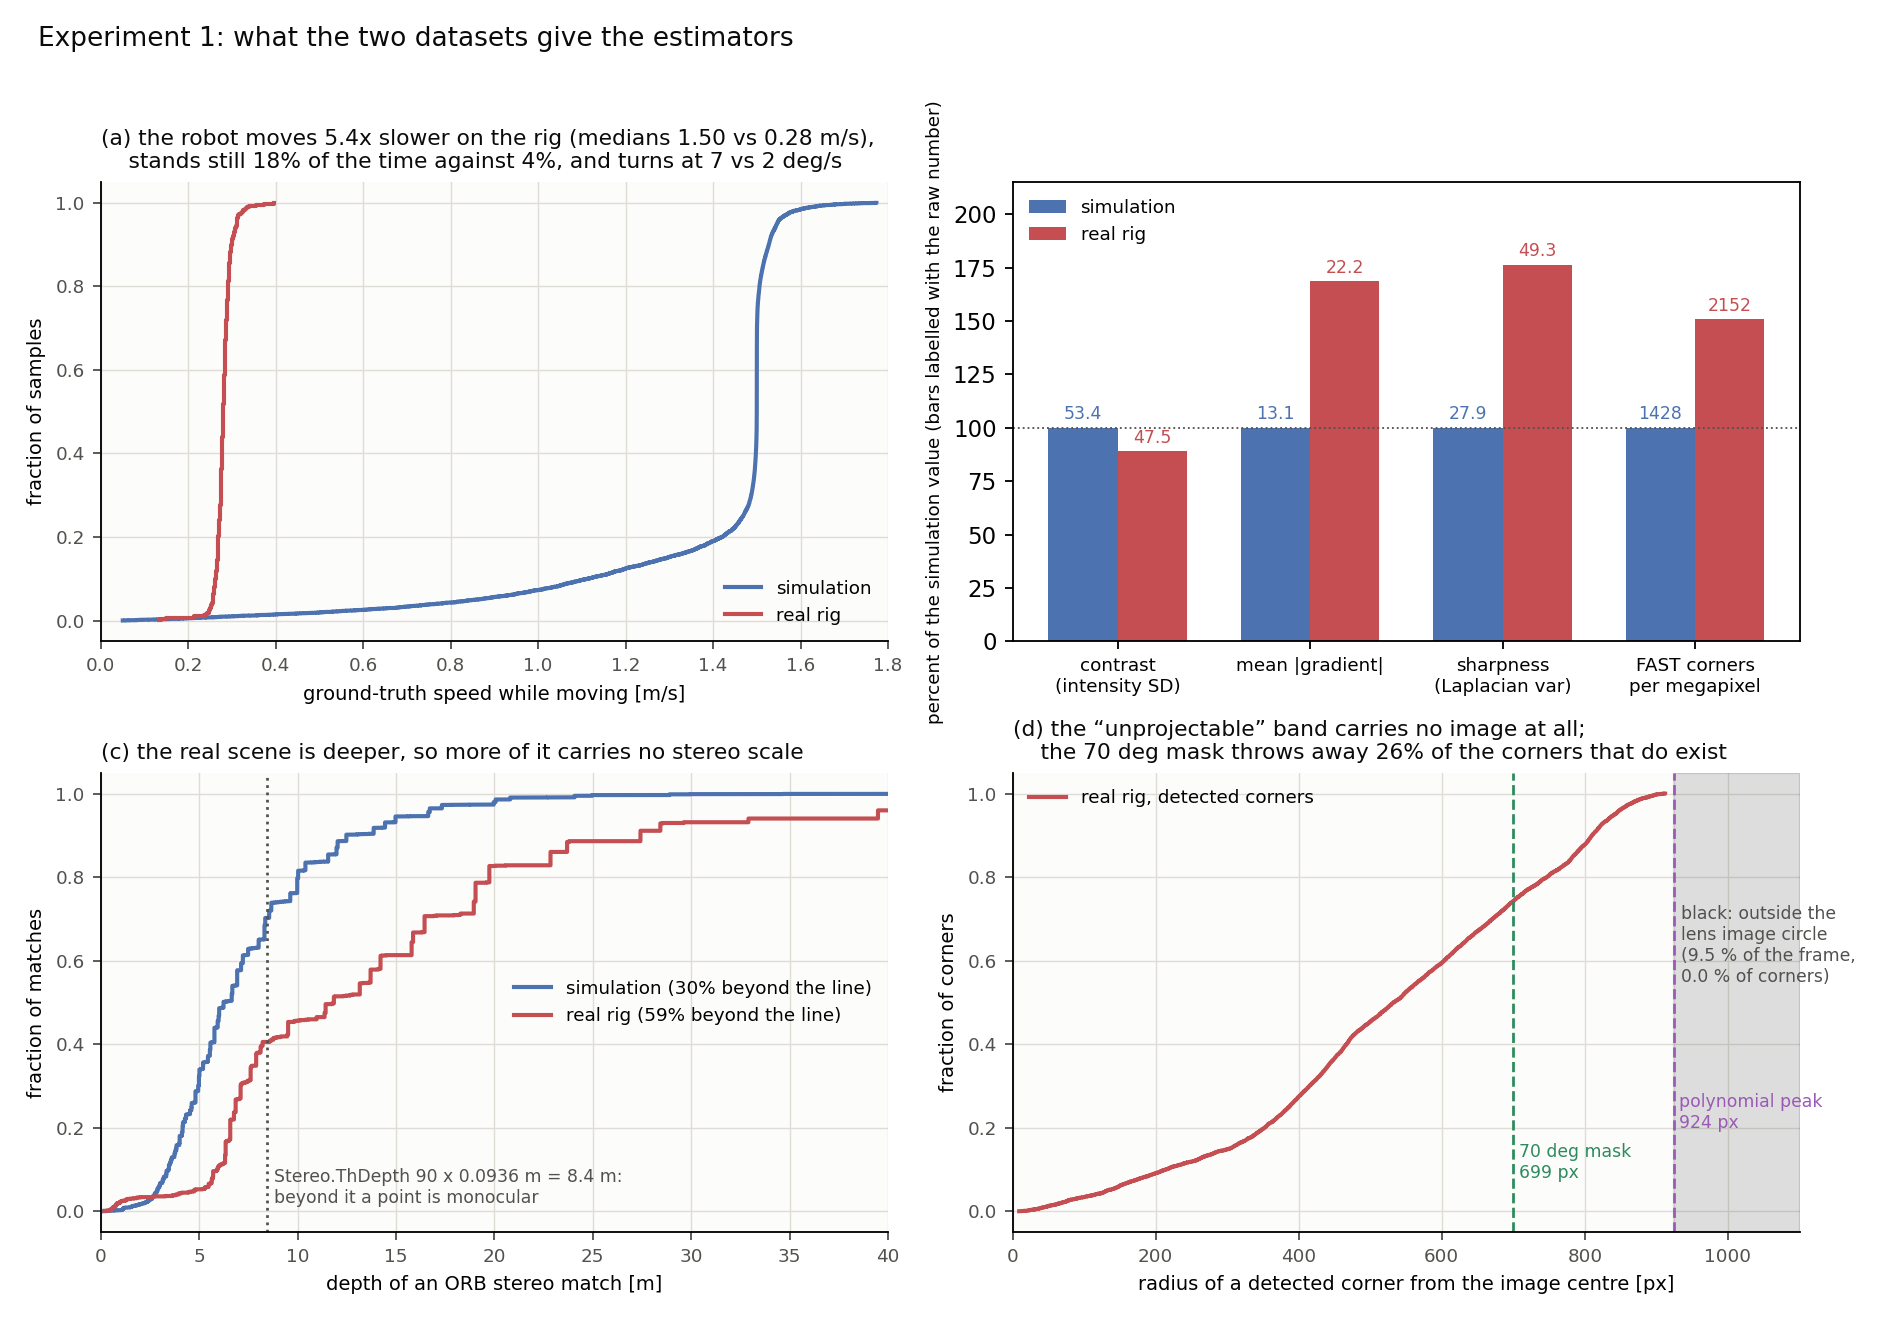
\includegraphics{exp1_dataset_compare.png}}%
  {Real frames: 169\,\% of sim gradient, \textbf{3$\times$} corners per frame;
   VINS holds 150 features 100\,\% of seconds. But 0.28 vs 1.50\,m/s
   $\Rightarrow$ \textbf{5.8$\times$} more IMU time per metre. 59\,\% of stereo
   matches beyond 8.4\,m (sim 30\,\%). Drift: 1.9$\times$ per second,
   10.5$\times$ per metre.}%
  {ORB-1 / VINS-1 have more corners than they use, so detection is not the
   limit. ORB-2 / VINS-2 integrate per \emph{second}: bias, gravity tilt and
   standing still all grow with time. ThDepth 90 $\times$ 0.0936\,m = 8.4\,m:
   beyond it ORB-1 stereo gives direction but no scale.}%
  {compare the two domains per second, never per metre.}
\end{frame}

% ---------------------------------------------------------------- R9
\begin{frame}[label=R9]{R9 \;ORB-1, 5, 6 \;Three rules for reading an ORB-SLAM3 number}
  \hl{ORB1}\hl{ORB5}\hl{ORB6}\orbstrip\par\vspace{0.6em}
  \centering\small
  \begin{tabular}{@{}p{0.27\textwidth} p{0.33\textwidth} p{0.33\textwidth}@{}}
    \toprule
    \textbf{Rule} & \textbf{Measured} & \textbf{Block behind it} \\
    \midrule
    1. Differences under \textbf{$\sim$0.25\,m} are noise &
    3 identical repeats: ORB spreads up to 0.277\,m (80\,\% of its mean); VINS 3--7\,\% &
    ORB-1 drops different frames each run (70--98\,\% kept), ORB-5 runs on its own thread; VINS took every frame \\
    \addlinespace
    2. Score rotation \textbf{after} the 90$^\circ$ step &
    rotation RMS 13--19$^\circ$, median 0.25--2.5$^\circ$ &
    ORB-6 switches the published frame from camera to gravity at init: a convention, not an error \\
    \addlinespace
    3. A path 2--5\,\% too long is \textbf{not} a scale error &
    after init: 0.997--0.999 local scale &
    the arc length of the pre-init spike (3--8\,m in the first 3.5\,s) \\
    \bottomrule
  \end{tabular}
  \src{Experiment 1 note: ``How repeatable is any of this?'', ``the rotation column'', ``the path excess is not a scale bias''.}
\end{frame}

% ---------------------------------------------------------------- R10
\begin{frame}[label=R10]{R10 \;RTAB-5 + RTAB-6 \;The words propose, the geometry disposes}
  \hl{RTAB5}\hl{RTAB6}\rtabstrip\par\vspace{0.2em}
  \finding{rtabc}{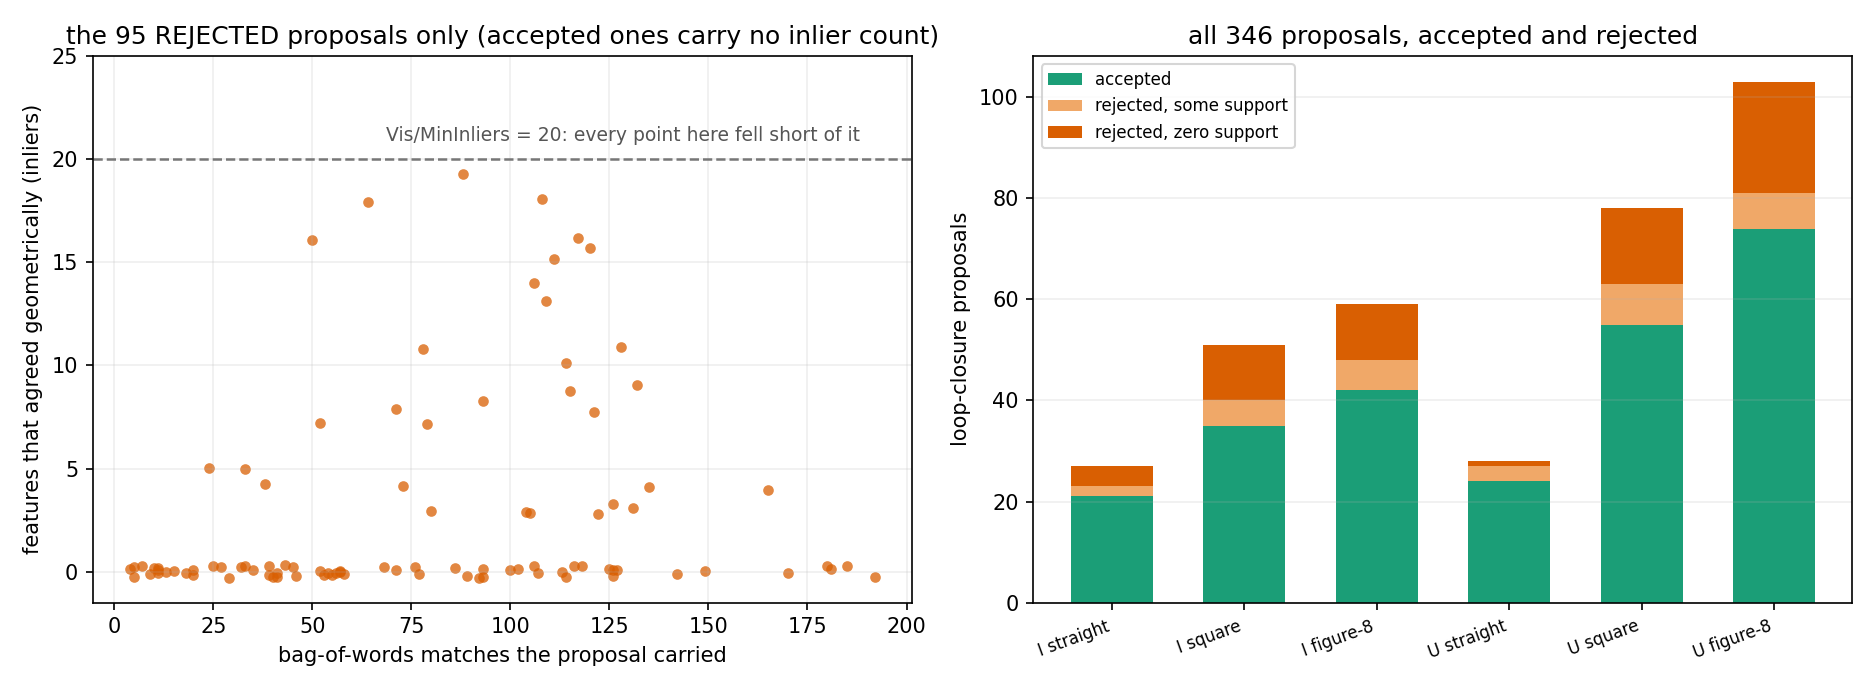
\includegraphics{exp4_rtabmap_gating.png}}%
  {6 relocalisation runs: 346 proposals, 251 accepted (73\,\%). Of the 95
   rejected, \textbf{64 had zero} features agreeing in metres, carrying a
   median of 77 matching words and up to 192.}%
  {RTAB-5 votes on shared words, and repeated rack faces give two aisles
   about 100 words in common. RTAB-6 checks in metres (MinInliers 20) and
   throws them out. This is the aliasing of \R{2}{}, caught here.
   MinInliers 35 stopped the warping but one bag then localised on 0 of 81
   poses.}%
  {inlier counts are logged only for rejections, so accepted proposals cannot be compared.}
\end{frame}

% ---------------------------------------------------------------- R11
\begin{frame}[label=R11]{R11 \;RTAB-3/8/9 + NAV-2 \;The first second poisons two layers}
  \hl{RTAB3}\hl{RTAB8}\hl{RTAB9}\rtabstrip\par\vspace{0.2em}
  \finding{rtabc}{%
  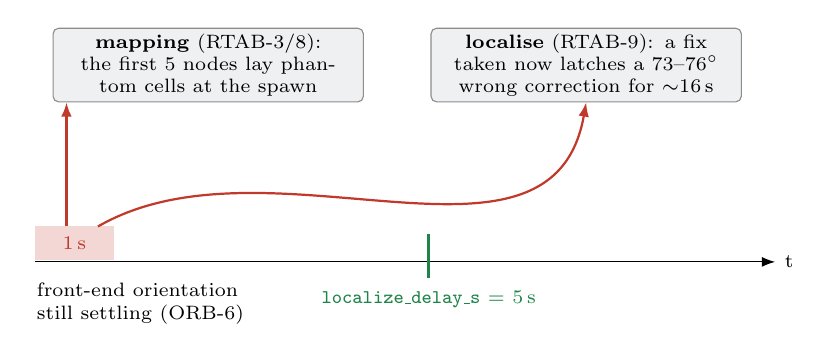
\begin{tikzpicture}[font=\scriptsize]
    \fill[bad!20] (0,0.02) rectangle (1.0,0.45); \node[text=bad] at (0.5,0.24) {1\,s};
    \draw[-{Latex}] (0,0) -- (9.4,0) node[right]{t};
    \node[anchor=north west, align=left] at (-0.1,-0.15) {front-end orientation\\still settling (ORB-6)};
    \node[box, text width=38mm, fill=mapcol!8] (map) at (2.2,2.5)
      {\textbf{mapping} (RTAB-3/8): the first 5 nodes lay phantom cells at the spawn};
    \node[box, text width=38mm, fill=mapcol!8] (loc) at (7.0,2.5)
      {\textbf{localise} (RTAB-9): a fix taken now latches a 73--76$^\circ$ wrong correction for $\sim$16\,s};
    \draw[arr, bad] (0.4,0.45) -- (map.south -| 0.4,0);
    \draw[arr, bad] (0.8,0.45) to[out=30, in=-100] (loc.south);
    \draw[good, very thick] (5.0,-0.2) -- (5.0,0.35);
    \node[text=good, anchor=north] at (5.0,-0.25) {\texttt{localize\_delay\_s} = 5\,s};
  \end{tikzpicture}}%
  {Localise: holding RTAB-Map back 5\,s cut the largest correction yaw from
   110--177$^\circ$ to 25$^\circ$ (3 runs). Map: 63--96\,\% of the phantom cells
   that block the spawn area came from the first five nodes.}%
  {Both layers consume the same unstable second. \texttt{wait\_for\_imu\_init}
   does not help (the flag is already true), and NAV-2's
   \texttt{init\_ignore\_s} acts only after the correction is formed.
   One rule for both: \textbf{do not consume the first second.}}%
  {the map-side fix (drop the first nodes' cells) is predicted by the data, not yet tested.}
\end{frame}

% ---------------------------------------------------------------- R12
\begin{frame}[label=R12]{R12 \;RTAB-8 $\rightarrow$ NAV-3 \;The poses are right, the grid is not}
  \hl{RTAB8}\hl{NAV3}\twostrips{\rtabstrip}{\navstrip}
  \finding{rtabc}{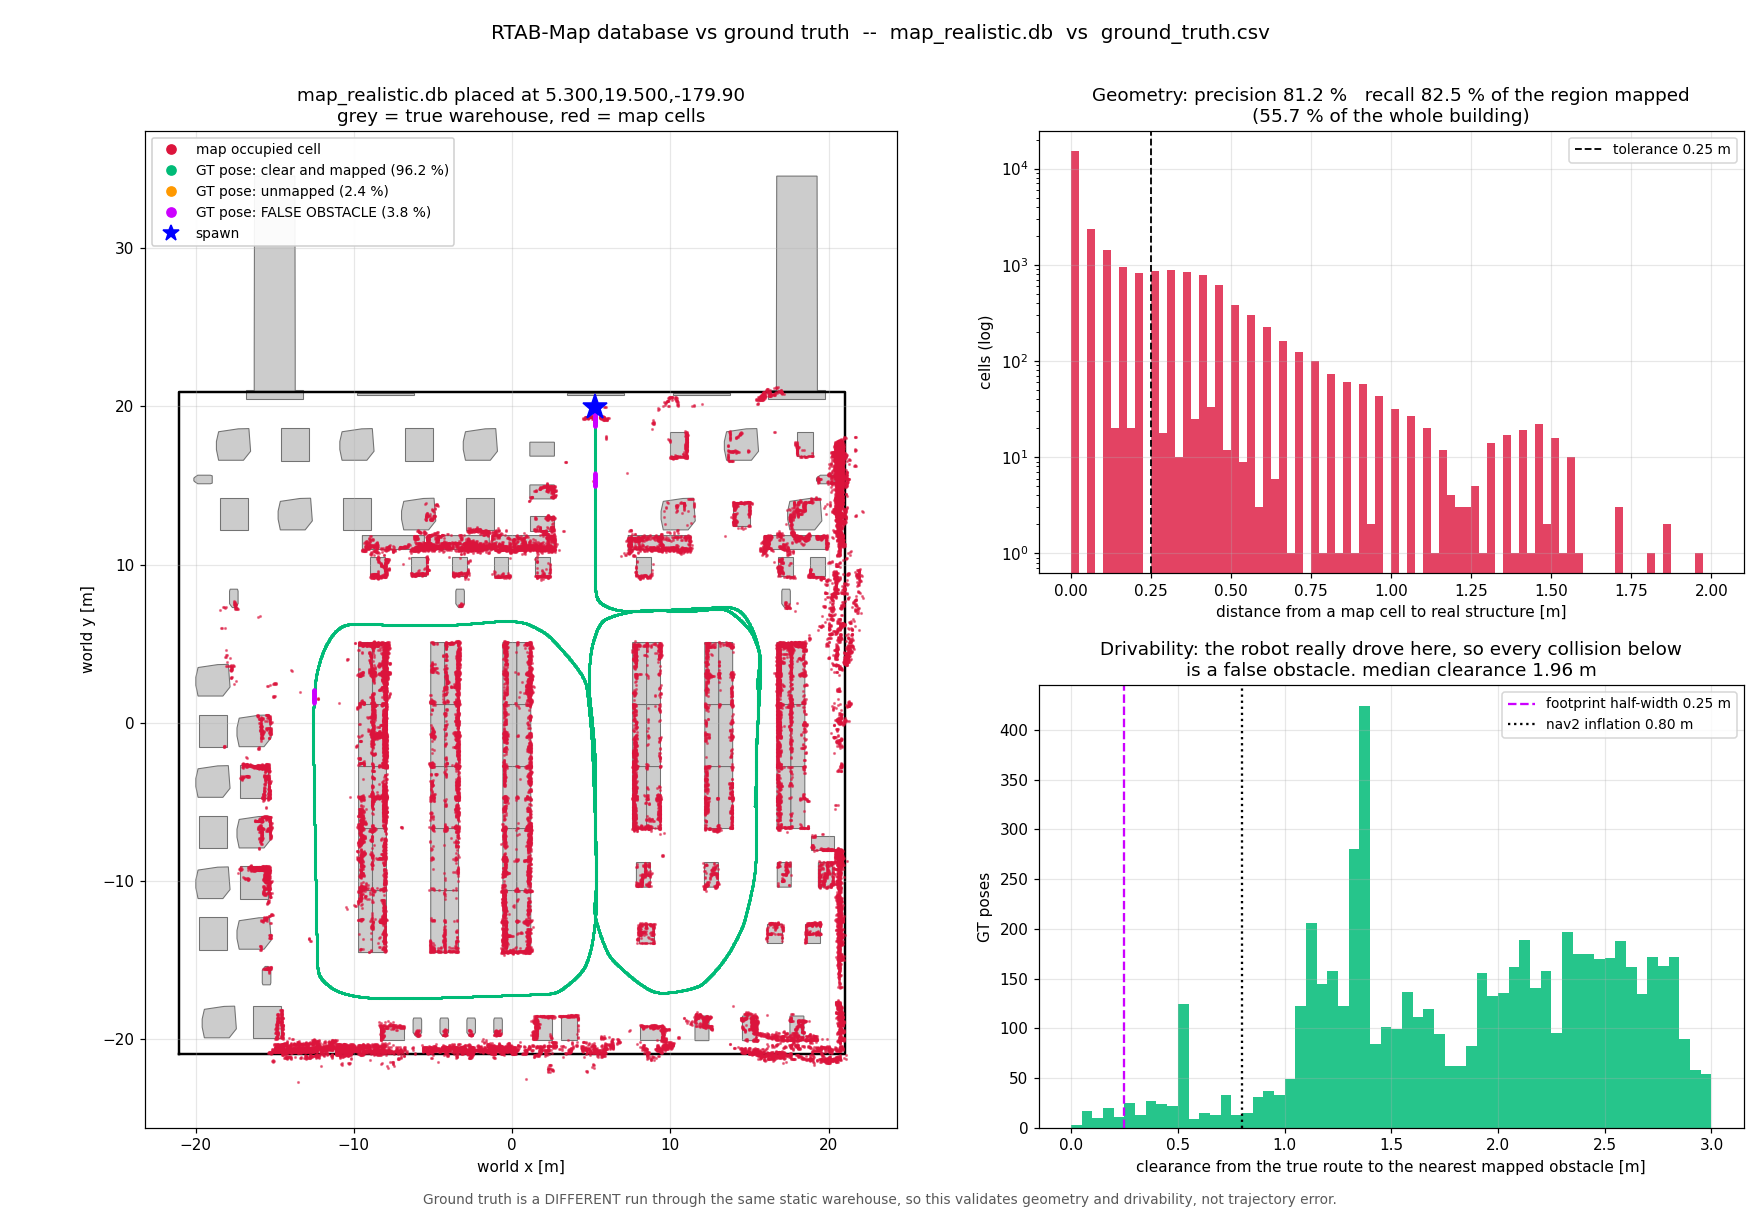
\includegraphics{map_realistic_validate.png}}%
  {4 closure-free maps. Graph poses \textbf{0.10--0.40\,m} rms over
   365--381\,m; a best fit improves them by $\le$\,0.012\,m. Grid precision
   77.8--84.8\,\% (target 90), false obstacles \textbf{3.8--10.2\,\%} (target 1):
   thickened shelves, walls $\sim$0.5\,m off, spawn phantoms.}%
  {The loss is made in RTAB-8, where depth images become cells
   (\texttt{Grid/RangeMax}, \texttt{MaxGroundHeight}, ray tracing), not in
   the trajectory. NAV-3 reads this \texttt{/map} with
   \texttt{allow\_unknown} false and 0.80\,m inflation: a phantom becomes a
   wall the planner must respect.}%
  {I-layout graphs have a 2.6--3.2\,m worst node; builds A/B changed 3 parameters at once.}
\end{frame}

% ---------------------------------------------------------------- R13
\begin{frame}[label=R13]{R13 \;RTAB-9 \;The pose is as good as the map behind it}
  \hl{RTAB9}\rtabstrip\par\vspace{0.2em}
  \finding{rtabc}{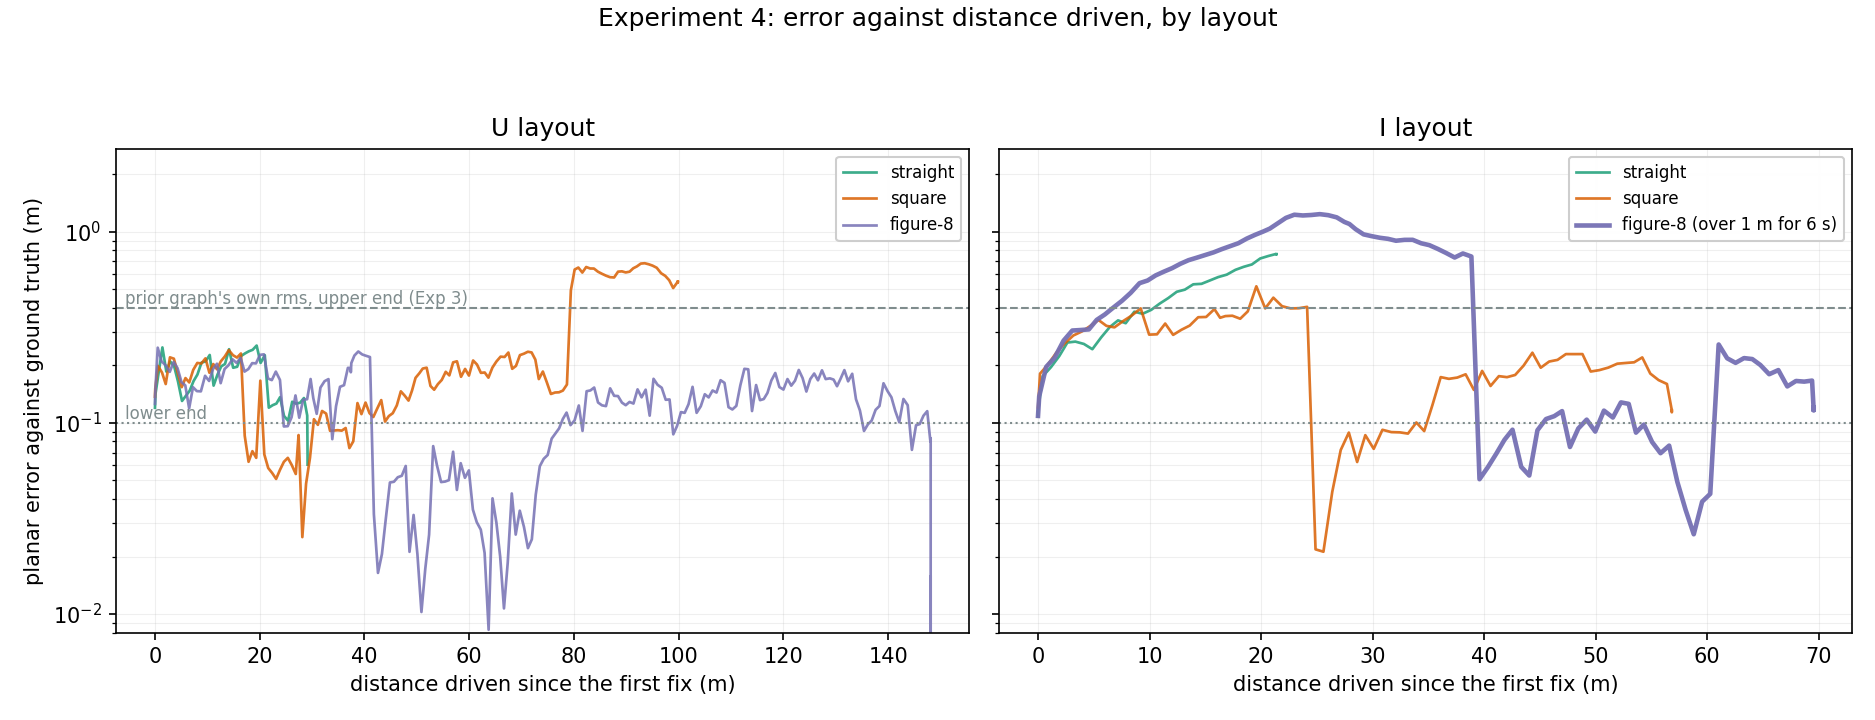
\includegraphics{exp4_error_vs_distance.png}}%
  {6 hand-driven runs, gate 1.5\,m: median error \textbf{0.13--0.21\,m},
   bounded in 5 of 6. One run over 1\,m for 6.5\,s, then back. Unaided ORB:
   the prior wins on all 4 routes $\ge$\,57\,m, loses the two shortest.}%
  {RTAB-9 can only match the map: graph 0.10--0.40\,m $\Rightarrow$ pose
   0.13--0.21\,m (\R{12}{}). The excursion is the gate's signature: a refused
   correction freezes map$\rightarrow$odom, the pose coasts on ORB odometry
   (ramp), then a fix is accepted (drop).}%
  {no repeats; a $\sim$0.1\,s timebase mismatch makes every figure an upper bound. Heading is worse on the I layout (1.3--2.8$^\circ$ vs 0.2--0.5$^\circ$), cause open.}
\end{frame}

% ---------------------------------------------------------------- R14
\begin{frame}[label=R14]{R14 \;What the results do not reach yet}
  \hl{NAV4}\hl{NAV5}\hl{NAV6}\hl{NAV7}\hl{NAV8}\navstrip\par\vspace{0.5em}
  \small
  \begin{itemize}\setlength{\itemsep}{0.35em}
    \item \textbf{NAV-4 \ldots\ NAV-8:} no goal was commanded in Experiment 4 (routes driven by
      hand), so the planner, controller and behaviour tree have no result. The open question
      from \R{12}{}: does a 3.8--10.2\,\% false-obstacle map block a route?
    \item \textbf{NAV-4 obstacle layer:} off in every run, so nothing tests a person in front of the robot.
    \item \textbf{Traffic in Experiment 4:} neither dynamic world was sampled.
    \item \textbf{VINS-3, 5, 6 and RTAB-4, 7:} no finding traced to them.
    \item \textbf{YOLO mask (Experiment 2):} it covers under a third of the moving pallet jacks'
      frames and none of the people, so the filtered arms are not reported.
  \end{itemize}
\end{frame}

% =============================================================================
% INDEX: one row per component, with the file that records it.  The empty
% column links each component to its findings R1..R14 (s7_results.tex).
% =============================================================================
\section{Index}

\begin{frame}{Index (1/2): the front ends --- and where each result attached}
  \centering
  \adjustbox{max width=\textwidth, max height=0.84\textheight}{%
  \begin{tabular}{l l l p{40mm}}
    \toprule
    ID & Component & Signal (file: field) & Results \\
    \midrule
    ORB-1 & features + stereo      & \repo{tracking_frontend.csv}: features; \repo{performance.csv}: frames processed & \R{1}{} \R{2}{} \R{3}{} \\
    ORB-2 & IMU preintegration     & \repo{performance.csv}: imu\_samples, imu\_starved & \R{2}{} \R{8}{} \\
    ORB-3 & tracking               & \repo{performance.csv}: tracking\_state; \repo{tracking_frontend.csv}: map\_matches\_inliers & \R{4}{} \R{8}{} \\
    ORB-4 & keyframe decision      & \repo{tracking_frontend.csv}: keyframes\_created & \\
    ORB-5 & local mapping, BA      & \repo{local_mapping.csv}: local\_ba\_ms & \R{3}{} \\
    ORB-6 & IMU initialisation     & \repo{performance.csv}: imu\_initialized, inertial\_ba1/2 & \R{3}{} \R{5}{} \R{6}{} \R{10}{} \\
    ORB-7 & place recognition      & \repo{loop_closing.csv}: detection events & \R{7}{} \\
    ORB-8 & loop correction, merge & \repo{loop_closing.csv}: correction\_translation\_m / \_rotation\_deg & \R{5}{} \R{7}{} \\
    \midrule
    VINS-1 & feature tracker       & \repo{frontend.csv}: feature\_count, stereo\_feature\_count & \R{2}{} \R{4}{} \R{8}{} \R{9}{} \\
    VINS-2 & IMU preintegration    & \repo{backend.csv}: imu\_wait\_ms, imu\_propagation\_ms & \R{2}{} \\
    VINS-3 & initialisation        & \repo{backend.csv}: initialized\_this\_frame; \repo{events.csv} & \\
    VINS-4 & sliding window        & \repo{backend.csv}: visual\_update\_ms; \repo{estimator_state.csv} & \R{4}{} \R{8}{} \R{9}{} \\
    VINS-5 & marginalisation       & \repo{backend.csv}: marginalization, keyframe & \\
    VINS-6 & time offset           & \repo{estimator_state.csv}: time\_delay\_s & \\
    VINS-7 & pose graph            & not run in our fork & \\
    \bottomrule
  \end{tabular}}
  \src{Both front ends also write \repo{vio.csv} (the pose) and \repo{run_summary.csv}.}
\end{frame}

\begin{frame}{Index (2/2): RTAB-Map and Nav2 --- and where each result attached}
  \centering
  \adjustbox{max width=\textwidth, max height=0.84\textheight}{%
  \begin{tabular}{l l l p{40mm}}
    \toprule
    ID & Component & Signal (file: field) & Results \\
    \midrule
    RTAB-1 & camera shim            & shim line in \repo{launch.log}; the TF tree & \\
    RTAB-2 & odometry in + sync     & TF waits in \repo{launch.log}; node count & \\
    RTAB-3 & new node               & database \texttt{Node} table & \R{10}{} \\
    RTAB-4 & memory                 & database \texttt{Info} / \texttt{Statistics} & \\
    RTAB-5 & detect (words)         & hypotheses in \repo{launch.log}; \repo{exp4_rtabmap_gating.py} & \R{11}{} \\
    RTAB-6 & verify (geometry)      & ``Not enough inliers'' in \repo{launch.log} & \R{11}{} \\
    RTAB-7 & graph optimisation     & ``Rejecting all added loop closures''; node poses & \\
    RTAB-8 & map assembly           & exported grid vs ground truth (Experiment 2A) & \R{10}{} \R{12}{} \R{13}{} \\
    RTAB-9 & output + gate          & \repo{gate_verdicts.csv}; \repo{localize_*.csv} & \R{10}{} \R{13}{} \\
    \midrule
    NAV-1 & inputs                  & TF tree; transform-timeout warnings & \\
    NAV-2 & pose gate               & \texttt{/localization\_ok}; the gate's log & \R{10}{} \\
    NAV-3 & global costmap          & published costmap & \R{12}{} \\
    NAV-4 & local costmap           & published costmap & \R{14}{} not measured \\
    NAV-5 & planner                 & \repo{outcome.json}: per goal & \R{14}{} not measured \\
    NAV-6 & controller              & \texttt{/cmd\_vel}; progress checker & \R{14}{} not measured \\
    NAV-7 & smoother + drive        & \repo{robot_gt.csv} & \R{14}{} not measured \\
    NAV-8 & behaviour tree          & \repo{outcome.json}; \texttt{bt\_navigator} log & \R{14}{} not measured \\
    \bottomrule
  \end{tabular}}
  \src{Experiment 2B runs live under \repo{map/<prior>/exp4/<world>_<route>_<config>/}.}
\end{frame}


\end{document}
